
\chapter{Python} 

\section{Overview}
Python is a widely used general-purpose, high-level programming language. Its design philosophy emphasizes code readability, and its syntax allows programmers to express concepts in fewer lines of code than would be possible in languages such as C. The language provides constructs intended to enable clear programs on both a small and large scale.

\vpara
Python supports multiple programming paradigms, including object-oriented, imperative and functional programming or procedural styles. It features a dynamic type system and automatic memory management and has a large and comprehensive standard library.

\vpara
Like other dynamic languages, Python is often used as a scripting language, but is also used in a wide range of non-scripting contexts. Using third-party tools, Python code can be packaged into standalone executable programs. Python interpreters are available for many operating systems.





\subsection{Downloading and installing mpMath}

mpmath is a free (BSD licensed) Python library for real and complex floating-point arithmetic with arbitrary precision. It has been developed by Fredrik Johansson since 2007, with help from many contributors. mpmath runs on Python 2.5 or higher (including Python 3.x), both on 32 and 64 bit, with no other required dependencies.

mpmath can be downloaded from

\vpara
\href{http://mpmath.org/}{http://mpmath.org/}.

The latest version is 0.19, released 2014-06-10. Download: mpmath-0.19.tar.gz., extract it, open a Windows command prompt in the extracted directory, and run
\begin{verbatim}
python setup.py install
\end{verbatim}


\vpara
The license is the New BSD License  can be found in appendix \ref{New BSD License})

The contributors are listed in section \ref{Contributors to mpMath}



\subsection{Running tests}

It is recommended that you run mpmath's full set of unit tests to make sure everything works. The tests are located in the tests subdirectory of the main mpmath directory. They can be run in the interactive interpreter using the runtests() function:


\lstset{language={Python}}
\begin{lstlisting}
import mpmath
mpmath.runtests()
\end{lstlisting}



\subsection{Precision management}

\subsubsection{autoprec()}

mpmath.autoprec(ctx, f, maxprec=None, catch=(), verbose=False)

\vpara
Return a wrapped copy of f that repeatedly evaluates f with increasing precision until the result converges to the full precision used at the point of the call.

\vpara
This heuristically protects against rounding errors, at the cost of roughly a 2x slowdown compared to manually setting the optimal precision. This method can, however, easily be fooled if the results from f depend 'discontinuously' on the precision, for instance if catastrophic cancellation can occur. Therefore, autoprec() should be used judiciously.

\vpara
\textbf{Examples}

\vpara
Many functions are sensitive to perturbations of the input arguments. If the arguments are decimal numbers, they may have to be converted to binary at a much higher precision. If the amount of required extra precision is unknown, autoprec() is convenient:

\lstset{language={Python}}
\begin{lstlisting}
>>> from mpmath import *
>>> mp.dps = 15
>>> mp.pretty = True
>>> besselj(5, 125 * 10**28) # Exact input
-8.03284785591801e-17
>>> besselj(5, '1.25e30') # Bad
7.12954868316652e-16
>>> autoprec(besselj)(5, '1.25e30') # Good
-8.03284785591801e-17
\end{lstlisting}


The following fails to converge because $\sin(\pi)=0$ whereas all finite-precision approximations of $\pi$ give nonzero values:

\lstset{language={Python}}
\begin{lstlisting}
>>> autoprec(sin)(pi)
Traceback (most recent call last):
...
NoConvergence: autoprec: prec increased to 2910 without convergence
\end{lstlisting}

As the following example shows, autoprec() can protect against cancellation, but is fooled by too severe cancellation:

\lstset{language={Python}}
\begin{lstlisting}
>>> x = 1e-10
>>> exp(x)-1; expm1(x); autoprec(lambda t: exp(t)-1)(x)
1.00000008274037e-10
1.00000000005e-10
1.00000000005e-10
>>> x = 1e-50
>>> exp(x)-1; expm1(x); autoprec(lambda t: exp(t)-1)(x)
0.0
1.0e-50
0.0
\end{lstlisting}

With catch, an exception or list of exceptions to intercept may be specified. The raised exception is interpreted as signaling insufficient precision. This permits, for example, evaluating a function where a too low precision results in a division by zero:

\lstset{language={Python}}
\begin{lstlisting}
>>> f = lambda x: 1/(exp(x)-1)
>>> f(1e-30)
Traceback (most recent call last):
...
ZeroDivisionError
>>> autoprec(f, catch=ZeroDivisionError)(1e-30)
1.0e+30
\end{lstlisting}


\subsubsection{workprec()}

mpmath.workprec(ctx, n, normalize\_output=False)

The block
\lstset{language={Python}}
\begin{lstlisting}
with workprec(n):
<code>
\end{lstlisting}
sets the precision to n bits, executes <code>, and then restores the precision.

\vpara
workprec(n)(f) returns a decorated version of the function f that sets the precision to n bits before execution, and restores the precision afterwards. With normalize\_output=True, it rounds the return value to the parent precision.

\subsection{workdps()}

mpmath.workdps(ctx, n, normalize\_output=False)

\vpara
This function is analogous to workprec (see documentation) but changes the decimal precision instead of the number of bits.


\subsubsection{extraprec()}

mpmath.extraprec(ctx, n, normalize\_output=False)

The block
\lstset{language={Python}}
\begin{lstlisting}
with extraprec(n):
<code>
\end{lstlisting}
increases the precision n bits, executes <code>, and then restores the precision.

\vpara
extraprec(n)(f) returns a decorated version of the function f that increases the working precision by n bits before execution, and restores the parent precision afterwards. With normalize\_output=True, it rounds the return value to the parent precision.

\subsubsection{extradps()}

mpmath.extradps(ctx, n, normalize\_output=False)

This function is analogous to extraprec (see documentation) but changes the decimal precision instead of the number of bits.

\subsection{Performance and debugging}

\subsubsection{memoize()}

mpmath.memoize(ctx, f)

\vpara
Return a wrapped copy of f that caches computed values, i.e. a memoized copy of f. Values are only reused if the cached precision is equal to or higher than the working precision:

\lstset{language={Python}}
\begin{lstlisting}
>>> from mpmath import *
>>> mp.dps = 15; mp.pretty = True
>>> f = memoize(maxcalls(sin, 1))
>>> f(2)
0.909297426825682
>>> f(2)
0.909297426825682
>>> mp.dps = 25
>>> f(2)
Traceback (most recent call last):
...
NoConvergence: maxcalls: function evaluated 1 times
\end{lstlisting}


\subsubsection{maxcalls()}

mpmath.maxcalls(ctx, f, N)

\vpara
Return a wrapped copy of f that raises NoConvergence when f has been called more than N times:

\lstset{language={Python}}
\begin{lstlisting}
>>> from mpmath import *
>>> mp.dps = 15
>>> f = maxcalls(sin, 10)
>>> print(sum(f(n) for n in range(10)))
1.95520948210738
>>> f(10)
Traceback (most recent call last):
...
NoConvergence: maxcalls: function evaluated 10 times
\end{lstlisting}


\subsubsection{monitor()}

mpmath.monitor(f, input='print', output='print')

\vpara
Returns a wrapped copy of f that monitors evaluation by calling input with every input (args, kwargs) passed to f and output with every value returned from f. The default action (specify using the special string value 'print') is to print inputs and outputs to stdout, along with the total evaluation count:

\lstset{language={Python}}
\begin{lstlisting}
>>> from mpmath import *
>>> mp.dps = 5; mp.pretty = False
>>> diff(monitor(exp), 1) # diff will eval f(x-h) and f(x+h)
in 0 (mpf('0.99999999906867742538452148'),) {}
out 0 mpf('2.7182818259274480055282064')
in 1 (mpf('1.0000000009313225746154785'),) {}
out 1 mpf('2.7182818309906424675501024')
mpf('2.7182808')
\end{lstlisting}


To disable either the input or the output handler, you may pass None as argument.

\vpara
Custom input and output handlers may be used e.g. to store results for later analysis:

\lstset{language={Python}}
\begin{lstlisting}
>>> mp.dps = 15
>>> input = []
>>> output = []
>>> findroot(monitor(sin, input.append, output.append), 3.0)
mpf('3.1415926535897932')
>>> len(input) # Count number of evaluations
9
>>> print(input[3]); print(output[3])
((mpf('3.1415076583334066'),), {})
8.49952562843408e-5
>>> print(input[4]); print(output[4])
((mpf('3.1415928201669122'),), {})
-1.66577118985331e-7
\end{lstlisting}

\subsubsection{timing()}

mpmath.timing(f, *args, **kwargs)

\vpara
Returns time elapsed for evaluating f(). Optionally arguments may be passed to time the execution of f(*args, **kwargs).

\vpara
If the first call is very quick, f is called repeatedly and the best time is returned.




\newpage
\section{CPython}

CPython, the reference implementation of Python, is free and open source software and has a community-based development model, as do nearly all of its alternative implementations. CPython is managed by the non-profit Python Software Foundation.

\vpara
For further information on Python, see \href{http://en.wikipedia.org/wiki/Python_(programming_language)}{Wikipedia: Python} (the text above has been copied from this reference), or the  \href{http://www.python.org/}{Python Homepage}. Support for COM is included in the distribution of the \href{http://www.activestate.com/activepython/downloads}{ActivePython Community Edition}.

\vpara
Python can use  GMP und MPFR thanks to \href{http://code.google.com/p/gmpy/}{GMPY2}, with documentation \href{https://gmpy2.readthedocs.org/en/latest/}{here}.

\vpara
IPython is an integrations platform for various scientific libraries (NumPy, SciPy, matlibplot, pandas etc.) \href{http://ipython.org/}{http://ipython.org/}. Popular distributions are the 

Community Edition of Anaconda: \href{http://docs.continuum.io/anaconda/index.html}{http://docs.continuum.io/anaconda/index.html}, 

%EPDFree (aka Canopy Express): \href{https://www.enthought.com/products/epd/free/}{https://www.enthought.com/products/epd/free/} 
%
%and Python(x, y): \href{https://code.google.com/p/pythonxy/}{https://code.google.com/p/pythonxy/}. 

\vpara
Book recommendation: \cite{McKinney2012}.

\vpara
Example for using the library

\lstset{language={Python}}
\begin{lstlisting}
#Enable COM support
from win32com.client import Dispatch

#Load the mpNumerics library
mp = Dispatch("mpNumerics.mp_Lib")

#Set Floating point type to MPFR with 60 decimal digits precision
mp.FloatingPointType = 3
mp.Prec10 = 60

#Assign values to x1 and x2
x1 = mp.Real(4.5)
x2 = mp.Real(1.21)

#Calculate x3 = x1 / x2
x3 = x1.Div(x2)

#Print the value of x3
print (x3.Str())
\end{lstlisting}

\vpara
Example for using Excel

\lstset{language={Python}}
\begin{lstlisting}
#Enable COM support
from win32com.client import Dispatch

#Load the Excel library
xl = Dispatch("Excel.Application")
xl.Visible = 1
xl.Workbooks.Add() 
xl.Cells(1,1).Value = "Hello442" 
print("From Python")
\end{lstlisting}



To compile the mpmath library libraries, Python 2.7 is required.

\subsection{Downloading and installing  CPython 2.7}
ActivePython is ActiveState's complete and ready-to-install distribution of Python. It provides a one-step installation of all essential Python modules, as well as extensive documentation. 
The Windows distribution ships with PyWin32 -- a suite of Windows tools developed by Mark Hammond, including bindings to the Win32 API and Windows COM. 
ActivePython can be downloaded from

\vpara
\href{http://www.activestate.com/activepython/downloads}{http://www.activestate.com/activepython/downloads}.

\vpara
The latest release version of the 2.7x series is 2.7.6.9. You need to download 2 separate files to support compilation of both 32 bit and 64 bit dlls.






\newpage
\subsection{Plotting}

If matplotlib is available, the functions plot and cplot in mpmath can be used to plot functions respectively as x-y graphs and in the complex plane. Also, splot can be used to
produce 3D surface plots.

\subsubsection{Function curve plots}

\begin{figure}[ht]
	\centering
	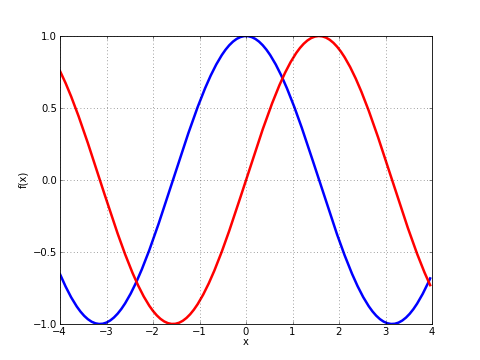
\includegraphics[scale=1.0]{Charts/png/MpMathPlot.png}
	\caption{MpMath 2Dplot}
	\label{Fig MpMath 2Dplot}
\end{figure}


Output of plot([cos, sin], [-4, 4])

\vpara
mpmath.plot(ctx, f, xlim=[-5, 5], ylim=None, points=200, file=None, dpi=None, singularities=[], axes=None)

\vpara
Shows a simple 2D plot of a function $f(x)$ or list of functions $[f_0(x),f_1(x),\ldots,f_n(x)]$ over a given interval specified by xlim. Some examples:

\lstset{language={Python}}
\begin{lstlisting}
plot(lambda x: exp(x)*li(x), [1, 4])
plot([cos, sin], [-4, 4])
plot([fresnels, fresnelc], [-4, 4])
plot([sqrt, cbrt], [-4, 4])
plot(lambda t: zeta(0.5+t*j), [-20, 20])
plot([floor, ceil, abs, sign], [-5, 5])
\end{lstlisting}


Points where the function raises a numerical exception or returns an infinite value are removed from the graph. Singularities can also be excluded explicitly as follows (useful
for removing erroneous vertical lines):

\lstset{language={Python}}
\begin{lstlisting}
plot(cot, ylim=[-5, 5]) # bad
plot(cot, ylim=[-5, 5], singularities=[-pi, 0, pi]) # good
\end{lstlisting}


For parts where the function assumes complex values, the real part is plotted with dashes and the imaginary part is plotted with dots.

Note: This function requires matplotlib (pylab).

\newpage
\subsubsection{Complex function plots}

\begin{figure}[ht]
	\centering
	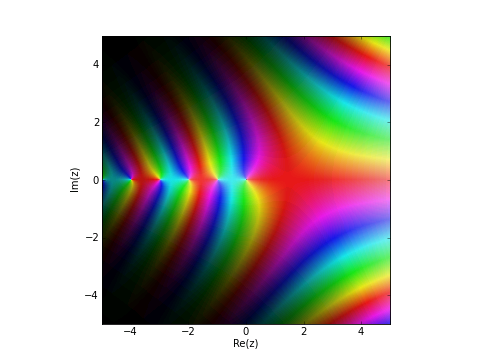
\includegraphics[scale=1.0]{Charts/png/MpMathCplot.png}
	\caption{MpMath cplot}
	\label{Fig MpMath cplot}
\end{figure}



Output of fp.cplot(fp.gamma, points=100000)

\vpara
mpmath.cplot(ctx, f, re=[-5, 5], im=[-5, 5], points=2000, color=None, verbose=False, file=None, dpi=None, axes=None)

\vpara
Plots the given complex-valued function f over a rectangular part of the complex plane specified by the pairs of intervals re and im. For example:

\lstset{language={Python}}
\begin{lstlisting}
cplot(lambda z: z, [-2, 2], [-10, 10])
cplot(exp)
cplot(zeta, [0, 1], [0, 50])
\end{lstlisting}


By default, the complex argument (phase) is shown as color (hue) and the magnitude is show as brightness. You can also supply a custom color function (color). This function should take a complex number as input and return an RGB 3-tuple containing floats in the range 0.0-1.0.

\vpara
To obtain a sharp image, the number of points may need to be increased to 100,000 or thereabout. Since evaluating the function that many times is likely to be slow, the 'verbose' option is useful to display progress.

Note: This function requires matplotlib (pylab).


\newpage
\subsubsection{3D surface plots}


Output of splot for the donut example.

\vpara
mpmath.splot(ctx, f, u=[-5, 5], v=[-5, 5], points=100, keep\_aspect=True, wireframe=False, file=None, dpi=None, axes=None)

\begin{figure}[ht]
	\centering
	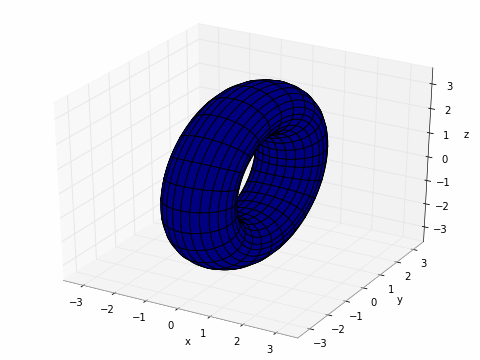
\includegraphics[scale=1.0]{Charts/png/MpMathSplot.png}
	\caption{MpMath Surface plot}
	\label{Fig MpMath Surface plot}
\end{figure}


Plots the surface defined by $f$.

\vpara
If $f$ returns a single component, then this plots the surface defined by $z=f(x,y)$ over the rectangular domain with $x=u$  and $y=v$.

\vpara
If $f$ returns three components, then this plots the parametric surface $x,y,z = f(u,v)$ over the pairs of intervals $u$ and $v$.

\vpara
For example, to plot a simple function:

\lstset{language={Python}}
\begin{lstlisting}
>>> from mpmath import *
>>> f = lambda x, y: sin(x+y)*cos(y)
>>> splot(f, [-pi,pi], [-pi,pi])
\end{lstlisting}


Plotting a donut:

\lstset{language={Python}}
\begin{lstlisting}
>>> r, R = 1, 2.5
>>> f = lambda u, v: [r*cos(u), (R+r*sin(u))*cos(v), (R+r*sin(u))*sin(v)]
>>> splot(f, [0, 2*pi], [0, 2*pi])
\end{lstlisting}


Note: This function requires matplotlib (pylab) 0.98.5.3 or higher.


\subsection{Using the C-API}

This document describes how to write modules in C or C++ to extend the Python interpreter with new modules. Those modules can not only define new functions but also new object types and their methods. The document also describes how to embed the Python interpreter in another application, for use as an extension language. Finally, it shows how to compile and link extension modules so that they can be loaded dynamically (at run time) into the interpreter, if the underlying operating system supports this feature.

This document assumes basic knowledge about Python. For an informal introduction to the language, see The Python Tutorial. The Python Language Reference gives a more formal definition of the language. The Python Standard Library documents the existing object types, functions and modules (both built-in and written in Python) that give the language its wide application range.

For a detailed description of the whole Python/C API, see the separate Python/C API Reference Manual.

. Extending Python with C or C++

It is quite easy to add new built-in modules to Python, if you know how to program in C. Such extension modules can do two things that can’t be done directly in Python: they can implement new built-in object types, and they can call C library functions and system calls.

To support extensions, the Python API (Application Programmers Interface) defines a set of functions, macros and variables that provide access to most aspects of the Python run-time system. The Python API is incorporated in a C source file by including the header "Python.h".

The compilation of an extension module depends on its intended use as well as on your system setup; details are given in later chapters.

Note:
The C extension interface is specific to CPython, and extension modules do not work on other Python implementations. In many cases, it is possible to avoid writing C extensions and preserve portability to other implementations. For example, if your use case is calling C library functions or system calls, you should consider using the ctypes module or the cffi library rather than writing custom C code. These modules let you write Python code to interface with C code and are more portable between implementations of Python than writing and compiling a C extension module.


\subsubsection{Downloading and installing Gmpy2}

GMPY and GMPY2 are C-coded Python extension modules that support fast multiple-precision arithmetic. GMPY only supports the GMP library and provides fast multiple-precision integer and rational arithmetic. The limited mpf type from GMP is also supported. GMPY2 supports the GMP library for integer and rational arithmetic but GMPY2 adds support for multiple-precision real and complex arithmetic as provided by the MPFR and MPC libraries. 

GMPY2 can be downloaded from

\vpara
\href{https://code.google.com/p/gmpy/}{https://code.google.com/p/gmpy/}.

The file which needs to downloaded is specific for the Python version. For Python 2.7x 32 bit, the file gmpy2-2.0.3.win32-py2.7.exe needs to be downloaded. After download, start the executable file and follow the instructions.

\vpara
The license can be found in appendix \ref{LGPLv3})

The contributors are listed in section \ref{Contributors to mpMath}





\subsection{Interfaces to the C family of languages}

\subsubsection{Windows, GNU/Linux, Mac OSX: GNU Compiler Collection}
The GNU Compiler Collection (GCC) is a compiler system produced by the GNU Project supporting various programming languages. GCC is a key component of the GNU toolchain. The Free Software Foundation (FSF) distributes GCC under the GNU General Public License (GNU GPL). GCC has played an important role in the growth of free software, as both a tool and an example.

\vpara
Originally named the GNU C Compiler, because it only handled the C programming language, GCC 1.0 was released in 1987 and the compiler was extended to compile C++ in December of that year.[1] Front ends were later developed for Objective-C, Objective-C++, Fortran, Java, Ada, and Go among others.[3]

\vpara
As well as being the official compiler of the unfinished GNU operating system, GCC has been adopted as the standard compiler by most other modern Unix-like computer operating systems, including Linux and the BSD family. A port to RISC OS has also been developed extensively in recent years. There is also an old (3.0) port of GCC to Plan9, running under its ANSI/POSIX Environment (APE).[4] GCC is also available for Microsoft Windows operating systems and for the ARM processor used by many portable devices.

\vpara
For further information on the GNU Compiler Collection, see \href{http://en.wikipedia.org/wiki/GNU_Compiler_Collection}{Wikipedia: GCC} (the text above has been copied from this reference), or the  \href{http://gcc.gnu.org/}{GCC Homepage}.


\subsubsection{Windows: MSVC}
Microsoft Visual C++ (often abbreviated as MSVC or VC++) is a commercial (free version available), integrated development environment (IDE) product from Microsoft for the C, C++, and C++/CLI programming languages. It features tools for developing and debugging C++ code, especially code written for the Microsoft Windows API, the DirectX API, and the Microsoft .NET Framework.

\vpara
Although the product originated as an IDE for the C programming language, the compiler's support for that language conforms only to the original edition of the C standard, dating from 1989. The later revisions of the standard, C99 and C11, are not supported.[41] According to Herb Sutter, the C compiler is only included for "historical reasons" and is not planned to be further developed. Users are advised to either use only the subset of the C language that is also valid C++, and then use the C++ compiler to compile their code, or to just use a different compiler such as Intel C++ Compiler or the GNU Compiler Collection instead.[42]

\vpara
For further information on Microsoft Visual C++, see \href{http://en.wikipedia.org/wiki/Visual_C\%2B\%2B}{Wikipedia: MSVC} (the text above has been copied from this reference), or the  \href{http://msdn.microsoft.com/en-us/vstudio/hh386302}{MSVC Homepage}.

\newpage
\subsubsection{Windows, GNU/Linux, Mac OSX: C}
In computing, C is a general-purpose programming language initially developed by Dennis Ritchie between 1969 and 1973 at AT\&T Bell Labs.[5][6] Like most imperative languages in the ALGOL tradition, C has facilities for structured programming and allows lexical variable scope and recursion, while a static type system prevents many unintended operations. Its design provides constructs that map efficiently to typical machine instructions, and therefore it has found lasting use in applications that had formerly been coded in assembly language, most notably system software like the Unix computer operating system.[7]

\vpara
C is one of the most widely used programming languages of all time,[8][9] and C compilers are available for the majority of available computer architectures and operating systems.

\vpara
Many later languages have borrowed directly or indirectly from C, including D, Go, Rust, Java, JavaScript, Limbo, LPC, C\#, Objective-C, Perl, PHP, Python, Verilog (hardware description language),[4] and Unix's C shell. These languages have drawn many of their control structures and other basic features from C. Most of them (with Python being the most dramatic exception) are also very syntactically similar to C in general, and they tend to combine the recognizable expression and statement syntax of C with underlying type systems, data models, and semantics that can be radically different. C++ and Objective-C started as compilers that generated C code; C++ is currently nearly a superset of C,[10] while Objective-C is a strict superset of C.[11]

\vpara
Before there was an official standard for C, many users and implementors relied on an informal specification contained in a book by Dennis Ritchie and Brian Kernighan; that version is generally referred to as "K\&R" C. In 1989 the American National Standards Institute published a standard for C (generally called "ANSI C" or "C89"). The next year, the same specification was approved by the International Organization for Standardization as an international standard (generally called "C90"). ISO later released an extension to the internationalization support of the standard in 1995, and a revised standard (known as "C99") in 1999. The current version of the standard (now known as "C11") was approved in December 2011.[12]


\vpara
For further information on C++, see \href{http://en.wikipedia.org/wiki/C_(programming_language)}{Wikipedia: C} (the text above has been copied from this reference), or the  \href{http://en.wikipedia.org/wiki/GNU_Compiler_Collection}{Wikipedia: GCC} (the text above has been copied from this reference), or the  \href{http://gcc.gnu.org/}{GCC Homepage}.



\vpara
Example in C


\lstset{language={C++}}
\begin{lstlisting}
#include <iostream>
#include "mpreal.h"

using mpfr::mpreal;    
using std::cout;
using std::endl;

// double - version
double schwefel(double x)
{
    return  418.9829 - x * sin(sqrt(abs(x)));
}
 
//MPFR C - version
void mpfr_schwefel(mpfr_t y, mpfr_t x)
{
   mpfr_t t;
   mpfr_init(t);
   mpfr_abs(t,x,GMP_RNDN);
   mpfr_sqrt(t,t,GMP_RNDN);
   mpfr_sin(t,t,GMP_RNDN);
   mpfr_mul(t,t,x,GMP_RNDN);
   mpfr_set_str(y,"418.9829",10,GMP_RNDN);
   mpfr_sub(y,y,t,GMP_RNDN);
   mpfr_clear(t);
}

// MPFR C++ - version
mpreal mpfr_schwefel(mpreal& x)
{
    return  "418.9829" - x*sin(sqrt(abs(x)));
}



int main(int argc, char* argv[])
{
    const int digits = 50; 
    mpreal::set_default_prec(mpfr::digits2bits(digits));
    const mpreal pi          =    mpfr::const_pi();
	mpreal x          =   "-343.5"; 
    mpreal SResult = mpfr_schwefel(x);
    cout.precision(digits);    // Show all the digits
    cout << "pi         =    "<<    pi          << endl;    
    cout << "SResult    =    "<<    SResult     << endl;   
    return 0;
}
\end{lstlisting}



\newpage
\subsubsection{Windows, GNU/Linux, Mac OSX: C++}
C++ (pronounced "see plus plus") is a statically typed, free-form, multi-paradigm, compiled, general-purpose programming language. It is regarded as an intermediate-level language, as it comprises both high-level and low-level language features.[3] Developed by Bjarne Stroustrup starting in 1979 at Bell Labs, C++ was originally named C with Classes, adding object oriented features, such as classes, and other enhancements to the C programming language. The language was renamed C++ in 1983,[4] as a pun involving the increment operator.

\vpara
C++ is one of the most popular programming languages[5][6] and is implemented on a wide variety of hardware and operating system platforms. As an efficient compiler to native code, its application domains include systems software, application software, device drivers, embedded software, high-performance server and client applications, and entertainment software such as video games.[7] Several groups provide both free and proprietary C++ compiler software, including the GNU Project, LLVM, Microsoft, Intel and Embarcadero Technologies. C++ has greatly influenced many other popular programming languages, most notably C\# and Java.

\vpara
C++ is also used for hardware design, where the design is initially described in C++, then analyzed, architecturally constrained, and scheduled to create a register-transfer level hardware description language via high-level synthesis.[8]

\vpara
The language began as enhancements to C, first adding classes, then virtual functions, operator overloading, multiple inheritance, templates and exception handling, among other features. After years of development, the C++ programming language standard was ratified in 1998 as ISO/IEC 14882:1998. The standard was amended by the 2003 technical corrigendum, ISO/IEC 14882:2003. The current standard extending C++ with new features was ratified and published by ISO in September 2011 as ISO/IEC 14882:2011 (informally known as C++11).[9]

\vpara
For further information on C++, see \href{http://en.wikipedia.org/wiki/C\%2B\%2B}{Wikipedia: C++} (the text above has been copied from this reference), or the  \href{http://gcc.gnu.org/}{GCC Homepage}.


\vpara
Example in C++


\lstset{language={C++}}
\begin{lstlisting}

#include <iostream>
#include "mpreal.h"

int main(int argc, char* argv[])
{
using mpfr::mpreal;    
using std::cout;
using std::endl;

// Required precision of computations in decimal digits
// Play with it to check different precisions
const int digits = 50; 

// Setup default precision for all subsequent computations
// MPFR accepts precision in bits - so we do the conversion 
mpreal::set_default_prec(mpfr::digits2bits(digits));

// Compute all the vital characteristics of mpreal (in current precision)
// Analogous to lamch from LAPACK
const mpreal one         =    1.0;
const mpreal zero        =    0.0;
const mpreal eps         =    std::numeric_limits<mpreal>::epsilon();
const int    base        =    std::numeric_limits<mpreal>::radix;
const mpreal prec        =    eps * base;
const int bindigits      =    std::numeric_limits<mpreal>::digits(); // eqv. to mpfr::mpreal::get_default_prec();
const mpreal rnd         =    std::numeric_limits<mpreal>::round_error();
const mpreal maxval      =    std::numeric_limits<mpreal>::max();
const mpreal minval      =    std::numeric_limits<mpreal>::min();
const mpreal small       =    one / maxval;
const mpreal sfmin       =    (small > minval) ? small * (one + eps) : minval;
const mpreal round       =    std::numeric_limits<mpreal>::round_style();
const int    min_exp     =    std::numeric_limits<mpreal>::min_exponent;
const mpreal underflow   =    std::numeric_limits<mpreal>::min();
const int    max_exp     =    std::numeric_limits<mpreal>::max_exponent;
const mpreal overflow    =    std::numeric_limits<mpreal>::max();

// Additionally compute pi with required accuracy - just for fun :)
const mpreal pi          =    mpfr::const_pi();

cout.precision(digits);    // Show all the digits
cout << "pi         =    "<<    pi          << endl;    
cout << "eps        =    "<<    eps         << endl;
cout << "base       =    "<<    base        << endl;
cout << "prec       =    "<<    prec        << endl;
cout << "b.digits   =    "<<    bindigits   << endl;
cout << "rnd        =    "<<    rnd         << endl;
cout << "maxval     =    "<<    maxval      << endl;    
cout << "minval     =    "<<    minval      << endl;    
cout << "small      =    "<<    small       << endl;    
cout << "sfmin      =    "<<    sfmin       << endl;    
cout << "1/sfmin    =    "<<    1 / sfmin   << endl;    
cout << "round      =    "<<    round       << endl;    
cout << "max_exp    =    "<<    max_exp     << endl;
cout << "min_exp    =    "<<    min_exp     << endl;
cout << "underflow  =    "<<    underflow   << endl;    
cout << "overflow   =    "<<    overflow    << endl;

return 0;
}

\end{lstlisting}



\newpage
\subsubsection{Mac OSX: Objective C}
Objective-C is a general-purpose, object-oriented programming language that adds Smalltalk-style messaging to the C programming language. It is the main programming language used by Apple for the OS X and iOS operating systems, and their respective application programming interfaces (APIs), Cocoa and Cocoa Touch.

\vpara
The programming language Objective-C was originally developed in the early 1980s. It was selected as the main language used by NeXT for its NeXTSTEP operating system, from which OS X and iOS are derived.[2] Generic Objective-C programs that do not use the Cocoa or Cocoa Touch libraries, or using parts that may be ported or reimplemented for other systems can also be compiled for any system supported by GCC or Clang.

\vpara
Objective-C source code program files usually have .m filename extensions, while Objective-C header files have .h extensions, the same as for C header files. Objective-C++ files are denoted with a .mm file extension.


\vpara
For further information on C++, see \href{http://en.wikipedia.org/wiki/Objective-C}{Wikipedia: Objective C} (the text above has been copied from this reference), or the  \href{http://gcc.gnu.org/}{GCC Homepage}.



\vpara
Example in Objective C

\lstset{language={C++}}
\begin{lstlisting}
# import "Forwarder.h"
# import "Recipient.h"
 
int main(void) {
 Forwarder *forwarder = [Forwarder new];
 Recipient *recipient = [Recipient new];
 
 [forwarder setRecipient:recipient]; //Set the recipient.
 /*
 * Observe forwarder does not respond to a hello message! It will
 * be forwarded. All unrecognized methods will be forwarded to
 * the recipient
 * (if the recipient responds to them, as written in the Forwarder)
 */
 [forwarder hello];
 
 [recipient release];
 [forwarder release];
 
 return 0;
}
\end{lstlisting}




\newpage
\subsubsection{Mac OSX: Objective C++}
Objective-C++ is a language variant accepted by the front-end to the GNU Compiler Collection and Clang, which can compile source files that use a combination of C++ and Objective-C syntax. Objective-C++ adds to C++ the extensions that Objective-C adds to C. As nothing is done to unify the semantics behind the various language features, certain restrictions apply:

A C++ class cannot derive from an Objective-C class and vice versa.

C++ namespaces cannot be declared inside an Objective-C declaration.

Objective-C declarations may appear only in global scope, not inside a C++ namespace

Objective-C classes cannot have instance variables of C++ classes that do not have a default constructor or that have one or more virtual methods,[citation needed] but pointers to C++ objects can be used as instance variables without restriction (allocate them with new in the -init method).

C++ "by value" semantics cannot be applied to Objective-C objects, which are only accessible through pointers.

An Objective-C declaration cannot be within a C++ template declaration and vice versa. However, Objective-C types, (e.g., Classname *) can be used as C++ template parameters.

Objective-C and C++ exception handling is distinct; the handlers of each cannot handle exceptions of the other type. This is mitigated in recent runtimes as Objective-C exceptions are either replaced by C++ exceptions completely (Apple runtime), or partly when Objective-C++ library is linked (GNUstep libobjc2).

Care must be taken since the destructor calling conventions of Objective-C and C++’s exception run-time models do not match (i.e., a C++ destructor will not be called when an Objective-C exception exits the C++ object’s scope). The new 64-bit runtime resolves this by introducing interoperability with C++ exceptions in this sense.[15]

Objective-C blocks and C++11 lambdas are distinct entities, however a block is transparently generated on Mac OS X when passing a lambda where a block is expected.[16]

Objective-C++ is Objective-C (probably with COCOA Framework) with the ability to link with C++ code (probable classes).

\vpara
Yes, you can use this language in XCODE to develop for Mac OS X, iPhone/iPodTouch, iPad. It works very well.

You don't have to do anything weird in your project to use Objective-C++. Just name your Objective-C files with the extension .mm (instead of .m) and you are good to go.

\vpara
It is my favorite architecture: develop base class library of my game/application in C++ so I can reuse it in other platforms (Windows, Linux) and use COCOA just for the iPhone/iPad UI specific stuff.



\vpara
For further information on Objective C++, see \href{http://en.wikipedia.org/wiki/C\%2B\%2B}{Wikipedia: C++} (the text above has been copied from this reference), or the  \href{http://gcc.gnu.org/}{GCC Homepage}.


\vpara
Example in C++


\lstset{language={C++}}
\begin{lstlisting}

#include <iostream>
#include "mpreal.h"

int main(int argc, char* argv[])
{
    using mpfr::mpreal;    
    using std::cout;
    using std::endl;
    
    // Required precision of computations in decimal digits
    // Play with it to check different precisions
    const int digits = 50; 

    // Setup default precision for all subsequent computations
    // MPFR accepts precision in bits - so we do the conversion 
    mpreal::set_default_prec(mpfr::digits2bits(digits));

    // Compute all the vital characteristics of mpreal (in current precision)
    // Analogous to lamch from LAPACK
    const mpreal one         =    1.0;
    const mpreal zero        =    0.0;
    const mpreal eps         =    std::numeric_limits<mpreal>::epsilon();
    const int    base        =    std::numeric_limits<mpreal>::radix;
    const mpreal prec        =    eps * base;
    const int bindigits      =    std::numeric_limits<mpreal>::digits(); // eqv. to mpfr::mpreal::get_default_prec();
    const mpreal rnd         =    std::numeric_limits<mpreal>::round_error();
    const mpreal maxval      =    std::numeric_limits<mpreal>::max();
    const mpreal minval      =    std::numeric_limits<mpreal>::min();
    const mpreal small       =    one / maxval;
    const mpreal sfmin       =    (small > minval) ? small * (one + eps) : minval;

    
    // Additionally compute pi with required accuracy - just for fun :)
    const mpreal pi          =    mpfr::const_pi();
        
    cout.precision(digits);    // Show all the digits
    cout << "pi         =    "<<    pi          << endl;    
    cout << "eps        =    "<<    eps         << endl;
    cout << "base       =    "<<    base        << endl;
    cout << "prec       =    "<<    prec        << endl;
    cout << "b.digits   =    "<<    bindigits   << endl;
    cout << "rnd        =    "<<    rnd         << endl;
    cout << "maxval     =    "<<    maxval      << endl;    
    cout << "minval     =    "<<    minval      << endl;    
    cout << "small      =    "<<    small       << endl;    
    cout << "sfmin      =    "<<    sfmin       << endl;    
    cout << "1/sfmin    =    "<<    1 / sfmin   << endl;    
 
    return 0;
}

\end{lstlisting}






\newpage
\section{Cython: C extensions for the Python language}

[Cython] is a programming language that makes writing C extensions for the Python language as easy as Python itself. It aims to become a superset of the [Python] language which gives it high-level, object-oriented, functional, and dynamic programming. Its main feature on top of these is support for optional static type declarations as part of the language. The source code gets translated into optimized C/C++ code and compiled as Python extension modules. This allows for both very fast program execution and tight integration with external C libraries, while keeping up the high programmer productivity for which the Python language is well known.

The primary Python execution environment is commonly referred to as CPython, as it is written in C. Other major implementations use Java (Jython [Jython]), C\# (IronPython [IronPython]) and Python itself (PyPy [PyPy]). Written in C, CPython has been conducive to wrapping many external libraries that interface through the C language. It has, however, remained non trivial to write the necessary glue code in C, especially for programmers who are more fluent in a high-level language like Python than in a close-to-the-metal language like C.

Originally based on the well-known Pyrex [Pyrex], the Cython project has approached this problem by means of a source code compiler that translates Python code to equivalent C code. This code is executed within the CPython runtime environment, but at the speed of compiled C and with the ability to call directly into C libraries. At the same time, it keeps the original interface of the Python source code, which makes it directly usable from Python code. These two-fold characteristics enable Cython’s two major use cases: extending the CPython interpreter with fast binary modules, and interfacing Python code with external C libraries.

While Cython can compile (most) regular Python code, the generated C code usually gains major (and sometime impressive) speed improvements from optional static type declarations for both Python and C types. These allow Cython to assign C semantics to parts of the code, and to translate them into very efficient C code. Type declarations can therefore be used for two purposes: for moving code sections from dynamic Python semantics into static-and-fast C semantics, but also for directly manipulating types defined in external libraries. Cython thus merges the two worlds into a very broadly applicable programming language.




\newpage
\section{PyPy: a fast alternative Python interpreter}


PyPy is a fast, compliant alternative implementation of the Python language (2.7.8 and 3.2.5). Thanks to its Just-in-Time compiler, Python programs often run faster on PyPy than on CPython.

PyPy’s Python Interpreter is written in RPython and implements the full Python language. This interpreter very closely emulates the behavior of CPython. It contains the following key components:
•a bytecode compiler responsible for producing Python code objects from the source code of a user application;
•a bytecode evaluator responsible for interpreting Python code objects;
•a standard object space, responsible for creating and manipulating the Python objects seen by the application.

The bytecode compiler is the preprocessing phase that produces a compact bytecode format via a chain of flexible passes (tokenizer, lexer, parser, abstract syntax tree builder, bytecode generator). The bytecode evaluator interprets this bytecode. It does most of its work by delegating all actual manipulations of user objects to the object space. The latter can be thought of as the library of built-in types. It defines the implementation of the user objects, like integers and lists, as well as the operations between them, like addition or truth-value-testing.

This division between bytecode evaluator and object space gives a lot of flexibility. One can plug in different object spaces to get different or enriched behaviours of the Python objects.


\subsection{Installation}

\subsubsection{Windows}

\subsubsection{Mac OSX}

\subsubsection{GNU/Linux}



\newpage
\section{Jython: Python for the Java Virtual Machine}

This list of JVM Languages comprises notable computer
programming languages that are used to produce
software that runs on the Java Virtual Machine (JVM).
Some of these languages are interpreted by a Java program,
and some are compiled to Java bytecode and JITcompiled
during execution as regular Java programs to
improve performance.
The JVM was initially designed to support only the Java
programming language. However, as time passed, ever
more languages were adapted or designed to run on the
Java platform.

Apart from the Java language itself, the most common or
well-known JVM languages are:

\begin{itemize}		
	\item Clojure, a Lisp dialect
	\item Groovy, a programming and scripting language
	\item Scala, an object-oriented and functional programming language[1]
	\item JRuby, an implementation of Ruby
	\item Jython, an implementation of Python
\end{itemize}

Jython is an implementation of the Python language for the Java platform. Throughout this book, you will be learning how to use the Python language, and along the way we will show you where the Jython implementation differs from CPython, which is the canonical implementation of Python written in the C language. It is important to note that the Python language syntax remains consistent throughout the different implementations. At the time of this writing, there are three mainstream implementations of Python. These implementations are: CPython, Jython for the Java platform, and IronPython for the .NET platform. At the time of this writing, CPython is the most prevalent of the implementations. Therefore if you see the word Python somewhere, it could well be referring to that implementation.

This book will reference the Python language in sections regarding the language syntax or functionality that is inherent to the language itself. However, the book will reference the name Jython when discussing functionality and techniques that are specific to the Java platform implementation. No doubt about it, this book will go in-depth to cover the key features of Jython and you’ll learn concepts that only adhere the Jython implementation. Along the way, you will learn how to program in Python and advanced techniques.

Developers from all languages and backgrounds will benefit from this book. Whether you are interested in learning Python for the first time or discovering Jython techniques and advanced concepts, this book is a good fit. Java developers and those who are new to the Python language will find specific interest in reading through Part I of this book as it will teach the Python language from the basics to more advanced concepts. Seasoned Python developers will probably find more interest in Part II and Part III as they focus more on the Jython implementation specifics. Often in this reference, you will see Java code compared with Python code.


\subsection{Installing Java}

\subsubsection{Windows}

\subsubsection{Mac OSX}

\subsubsection{GNU/Linux}



\subsection{Installing Eclipse with support for JPython}


\subsubsection{Windows}

\subsubsection{Mac OSX}

\subsubsection{GNU/Linux}





\newpage
\section{IronPython: Python for .NET Framework and Mono}


IronPython is an implementation of the Python programming language targeting the .NET Framework and Mono. Jim Hugunin created the project and actively contributed to it up until Version 1.0 which was released on September 5, 2006.[2] Thereafter, it was maintained by a small team at Microsoft until the 2.7 Beta 1 release; Microsoft abandoned IronPython (and its sister project IronRuby) in late 2010, after which Hugunin left to work at Google.[3] IronPython 2.0 was released on December 10, 2008.[4] The project is currently maintained by a group of volunteers at Microsoft's CodePlex open-source repository. It is free and open-source software, and can be implemented with Python Tools for Visual Studio, which is a free and open-source extension for free, isolated, and commercial versions of Microsoft's Visual Studio IDE.[5] [6]

IronPython is written entirely in C\#, although some of its code is automatically generated by a code generator written in Python.

IronPython is implemented on top of the Dynamic Language Runtime (DLR), a library running on top of the Common Language Infrastructure that provides dynamic typing and dynamic method dispatch, among other things, for dynamic languages.[7] The DLR is part of the .NET Framework 4.0 and is also a part of trunk builds of Mono. The DLR can also be used as a library on older CLI implementations.

For further information, see \href{http://en.wikipedia.org/wiki/IronPython}{Wikipedia: IronPython} (the text above has been copied from this reference).

The original distribution of SharpDevelop includes IronPython (it is not included in the mpFormulaPy IDE). Ironpython can be downloaded from the 
\href{http://ironpython.net/}{IronPython Homepage}. Visual Studio integration is available through  \href{http://ironpython.net/tools/}{Python Tools for Visual Studio}.


\lstset{language={Python}}
\begin{lstlisting}
#Load CLR
import clr

#Load the mpNumerics library
clr.AddReference('MatrixClass2')
from MatrixClass2 import mp, mpNum

#Set Floating point type to MPFR with 60 decimal digits precision
mp.FloatingPointType = 3;
mp.Prec10 = 60;

#Assign values to x1 and x2
x1 = mp.CNum("32.47");
x2 = mp.CNum("12.41");

#Calculate x3 = x1 / x2
x3 = x1 / x2;

#Print the value of x3
print "Result: ", x3.Str();
\end{lstlisting}





\newpage
\section{Brython: a Python to JavaScript compiler}

Brython is a Python to JavaScript compiler, but it does the whole job in the browser and so makes Python appear to be a client scripting language. 

Brythonic is an ancient Celtic language, but in this case Brython stands for Browser Python, or I suppose it could be reference to the Life of Brian. Wherever the name derives, Brython is another of the growing examples of treating JavaScript as an assembly language. In this case, though, the approach is slightly different. The idea is that you can write Python in the browser as if it was a language with built-in browser support. 

For example:

\lstset{language={Python}}
\begin{lstlisting}
<script type="text/python">
def echo():
alert("Hello %s !" %doc["zone"].value) </script>
\end{lstlisting}

You can see that this looks like a native script. You can also see that it is Python with a few extensions to enable it to work in the browser environment - doc represents the DOM and you can use it to select an element using indexing doc["zone"] is the element with id "zone". 








\newpage
\section{QPython: Python for Android}

QPython is a script engine that runs Python on android devices. It lets your android device run Python scripts and projects. It contains the Python interpreter, console, editor, and the SL4A Library for Android. It’s Python on Android! It offers the development kit which lets you easily develop Python projects and scripts on your Android device.


[[ Main Features ]] 

* Supports Python programming on Android including web apps, games, and SL4A programming etc * Run Python scripts / projects on Android devices 

* Can execute Python code \& files from QRCode 

* QEdit lets you create/edit Python scripts / projects easily 

* Includes many useful python libraries 

* Support pip 

[[ Programming Features ]] 

* Supports Web App programming, which let you develop mobile apps with web development framework, this speeds up your mobile development greatly 

* Supports native UI programming, which let you develop games more easily by using scripts 

* Supports SL4A programming to access Android’s features: network, Bluetooth, GPS, and more



\newpage
\section{Pythonista: Python for iOS}

Pythonista is an integrated development environment for writing Python scripts on iOS. You can create interactive experiments and prototypes using multi-touch, animations, and sound – or just use the interactive prompt as a powerful calculator.

With extensive support for URL schemes, access to the iOS clipboard and photo library, and all the powerful libraries that come with Python, it is also possible to use Pythonista as a flexible automation tool for text or image processing.

Pythonista is also an excellent companion for learning the Python language – You can get started easily with lots of ready-to-run examples, the interactive prompt helps you experiment, and you can read the entire documentation right within the app.

The code editor has everything you'd expect: Syntax highlighting, code completion and an extended keyboard specifically designed for writing Python. You can even extend the editor with your own scripts.

The Standard Library has tons of modules for doing math, processing text, working with data from the web, and much more. Additionally, you have access to the iOS clipboard, an in-app web browser and the powerful Python Imaging Library — including support for accessing photos in your camera roll.

Pythonista includes the NumPy and matplotlib packages for scientific computation and data visualization. 

With the integrated UI Editor, you can create user interfaces for your scripts without writing any code.





\chapter{LibreOffice Calc and Microsoft Excel}
\label{Spreadsheets} 


\section{LibreOffice Calc}
The mpFormulaPy library provides multiprecision arithmetic versions of  functions which are equivalent to the numerically orientated functions of LibreOffice Calc.


\subsection{Windows}
Installation on Windows, LibreOffice Portable:

The mpmath directory needs to be copied into the LibreOffice Python site-packages directory:
\begin{verbatim}
\LibreOfficePortable\App\libreoffice\program\python-core-3.3.3\lib\site-packages
\end{verbatim}
If you want gmpy2 support, copy the files 
\begin{verbatim}
gmpy2.pyd
gmpy2-2.0.5-py3.3.egg-info
\end{verbatim}
into the same directory.
	
The \verb|sheetFunction.py| file needs to be copied into the  LibreOffice Python Scripts directory:
\begin{verbatim}
\LibreOfficePortable\App\libreoffice\share\Scripts\python
\end{verbatim}


\subsection{Mac OSX}
Installation on the Macintosh:

In Finder, navigate to:
\begin{verbatim}
Macintosh HD/Applications/LibreOffice
\end{verbatim}	
Right-Click on LibreOffice, and choose 'Show Package Contents'. This will open the LibreOffice  'Contents' subdirectory.
The mpmath directory needs to be copied into the Python site-packages directory:
\begin{verbatim}
Contents/Frameworks/LibreOfficePython.framework/Versions/3.3/lib/python3.3/site-packages
\end{verbatim}
The \verb|sheetFunction.py| file needs to be copied into the  LibreOffice Python Scripts directory:
\begin{verbatim}
Contents/Resources/Scripts/Python
\end{verbatim}


\subsection{GNU/Linux}
Installation on Ubuntu 14.04

To install support for python scripting from within LibreOffice:
\begin{verbatim}
sudo apt-get install libreoffice-script-provider-python
\end{verbatim}

To install mpmath for Python 3.x:
\begin{verbatim}
sudo apt-get install python3-mpmath
\end{verbatim}

if nautilus is not already working, do the following:
\begin{verbatim}
sudo mkdir -p /root/.config/nautilus
gksu nautilus
\end{verbatim}

if gksu was not already installed, you need to install it:
\begin{verbatim}
sudo apt-get install gksu
\end{verbatim}

The \verb|sheetFunction.py| file needs to be copied into the LibreOffice Python Scripts directory:
\begin{verbatim}
Computer/usr/lib/libreoffice/share/Scripts/python
\end{verbatim}



\newpage
\section{Microsoft Excel}
The mpFormulaPy library provides multiprecision arithmetic versions of  functions which are equivalent to the numerically orientated functions of MS Excel.


\subsection{Windows}
The functions are enabled by selecting and activating the mpFormula32.xll or mpFormula64.xll Addin.


\subsection{Mac OSX}
The connection to MS Excel on OSX still needs to be worked out.




\newpage
\section{Spreadsheet functions implemented in mpFormulaPy}
\label{Using Spreadsheet functions}
The mpFormulaPy library provides multiprecision arithmetic versions of  functions which are equivalent to the numerically orientated functions of MS Excel and OpenOffice Calc.


\subsection{Spreadsheet Mathematical Functions}
The mathematical functions listed below are supported by MS Excel 2013, Apache Open Office 4.0, and LibreOffice 4.1. Earlier versions of these programs support a subset of these functions.
All of these functions have multiprecision arithmetic equivalents in mpFormulaPy.

\label{tab:Spreadsheet Mathematical Functions}%
\begin{center}
	\begin{longtable}{l l l }
		\caption{Spreadsheet Mathematical Functions}\\
		\hline
		\noalign{\vskip 1.5mm}
		\textbf{Function} & \textbf{Description} & \textbf{Section}  \\
		\noalign{\vskip 0.8mm}
		\hline
		\noalign{\vskip 1mm}
		\endfirsthead
		\multicolumn{3}{c}%
		{\tablename\ \thetable\ -- \textit{Continued from previous page}} \\
		\hline
		\noalign{\vskip 1.5mm}
		\textbf{Function} & \textbf{Description} & \textbf{Section}  \\
		\noalign{\vskip 0.8mm}
		\hline
		\noalign{\vskip 1mm}
		\endhead
		\hline \multicolumn{3}{r}{\textit{Continued on next page}} \\
		\endfoot
		\hline
		\endlastfoot
		ABS   & Returns the absolute value of a number &  \ref{ABS} (page \pageref{ABS}) \index{Spreadsheet Functions!ABS}\\
		ACOS  & Returns the arccosine of a number &  \ref{ACOS} (page \pageref{ACOS}) \index{Spreadsheet Functions!ACOS} \\
		ACOSH & Returns the inverse hyperbolic cosine of a number &  \ref{ACOSH} (page \pageref{ACOSH}) \index{Spreadsheet Functions!ACOSH} \\
		ACOT   & Returns the inverse cotangent of a number &  \ref{ACOT} (page \pageref{ACOT}) \index{Spreadsheet Functions!ACOT} \\
		ACOTH  & Returns the inverse hyperbolic cotangent of a  &  \ref{ACOTH} (page \pageref{ACOTH}) \index{Spreadsheet Functions!ACOTH} \\
		& number &   \\
		ASIN  & Returns the arcsine of a number &  \ref{ASIN} (page \pageref{ASIN}) \index{Spreadsheet Functions!ASIN} \\
		ARABIC  & Returns a Roman number to Arabic, as a number &  \ref{ARABIC} (page \pageref{ARABIC}) \index{Spreadsheet Functions!ARABIC} \\
		ASINH & Returns the inverse hyperbolic sine of a number &  \ref{ASINH} (page \pageref{ASINH}) \index{Spreadsheet Functions!ASINH} \\
		ATAN  & Returns the arctangent of a number &  \ref{ATAN} (page \pageref{ATAN}) \index{Spreadsheet Functions!ATAN} \\
		ATAN2 & Returns the arctangent from x- and y-coordinates &  \ref{ATAN2} (page \pageref{ATAN2}) \index{Spreadsheet Functions!ATAN2} \\
		ATANH & Returns the inverse hyperbolic tangent of a number &  \ref{ATANH} (page \pageref{ATANH}) \index{Spreadsheet Functions!ATANH} \\
		BASE  & Converts a number into a text representation with &  \ref{BASE} (page \pageref{BASE}) \index{Spreadsheet Functions!BASE} \\
		& the given radix (base)  &   \\
		CEILING & Rounds a number to the nearest integer or to the &  \ref{CEILING} (page \pageref{CEILING}) \index{Spreadsheet Functions!CEILING} \\
		& nearest multiple of significance &   \\
		CEILING.MATH & Rounds a number to the nearest integer or to the &  \ref{CEILING.MATH} (page \pageref{CEILING.MATH}) \index{Spreadsheet Functions!CEILING.MATH} \\
		& nearest multiple of significance &   \\
		COMBIN & Returns the number of combinations for a given &  \ref{COMBIN} (page \pageref{COMBIN}) \index{Spreadsheet Functions!COMBIN} \\
		& number of objects &  \\
		COMBINA & Returns the number of combinations with &  \ref{COMBINA} (page \pageref{COMBINA}) \index{Spreadsheet Functions!COMBINA} \\
		& repetitions for a given number of objects &  \\
		COS   & Returns the cosine of a number &  \ref{COS} (page \pageref{COS}) \index{Spreadsheet Functions!COS} \\
		COSH  & Returns the hyperbolic cosine of a number &  \ref{COSH} (page \pageref{COSH}) \index{Spreadsheet Functions!COSH} \\
		COT   & Returns the cotangent of a number &  \ref{COT} (page \pageref{COT}) \index{Spreadsheet Functions!COT} \\
		COTH  & Returns the hyperbolic cotangent of a number &  \ref{COTH} (page \pageref{COTH}) \index{Spreadsheet Functions!COTH} \\
		CSC  & Returns the cosecant of a number &  \ref{CSC} (page \pageref{CSC}) \index{Spreadsheet Functions!CSC} \\
		CSCH  & Returns the hyperbolic cosecant of a number &  \ref{CSCH} (page \pageref{CSCH}) \index{Spreadsheet Functions!CSCH} \\
		DECIMAL & Converts a text representation of a number in &  \ref{DECIMAL} (page \pageref{DECIMAL}) \index{Spreadsheet Functions!DECIMAL} \\
		& a given base into a decimal number &   \\
		DEGREES & Converts radians to degrees &  \ref{DEGREES} (page \pageref{DEGREES}) \index{Spreadsheet Functions!DEGREES} \\
		EVEN  & Rounds a number up to the nearest even integer &  \ref{EVEN} (page \pageref{EVEN}) \index{Spreadsheet Functions!EVEN} \\
		EXP   & Returns e raised to the power of a given number &  \ref{EXP} (page \pageref{EXP}) \index{Spreadsheet Functions!EXP} \\
		FACT  & Returns the factorial of a number &  \ref{FACT} (page \pageref{FACT}) \index{Spreadsheet Functions!FACT} \\
		FACTDOUBLE & Returns the double factorial of a number &  \ref{FACTDOUBLE} (page \pageref{FACTDOUBLE}) \index{Spreadsheet Functions!FACTDOUBLE} \\
		FLOOR & Rounds a number down, toward zero &  \ref{FLOOR} (page \pageref{FLOOR}) \index{Spreadsheet Functions!FLOOR} \\
		FLOOR.MATH & Rounds a number down, to the nearest integer or  &  \ref{FLOOR.MATH} (page \pageref{FLOOR.MATH}) \index{Spreadsheet Functions!FLOOR.MATH} \\
		& to the nearest multiple of significance &   \\
		GCD   & Returns the greatest common divisor &  \ref{GCD} (page \pageref{GCD}) \index{Spreadsheet Functions!GCD} \\
		GCD\_ADD   & *Returns the greatest common divisor &  \ref{GCD} (page \pageref{GCD}) \index{Spreadsheet Functions!GCD\_ADD} \\
		INT   & Rounds a number down to the nearest integer &  \ref{INT} (page \pageref{INT}) \index{Spreadsheet Functions!INT} \\
		LCM   & Returns the least common multiple &  \ref{LCM} (page \pageref{LCM}) \index{Spreadsheet Functions!LCM} \\
		LCM\_ADD   & *Returns the least common multiple &  \ref{LCM} (page \pageref{LCM}) \index{Spreadsheet Functions!LCM\_ADD} \\
		LN    & Returns the natural logarithm of a number &  \ref{LN} (page \pageref{LN}) \index{Spreadsheet Functions!LN} \\
		LOG   & Returns the logarithm of a number to a specified &  \ref{LOG} (page \pageref{LOG}) \index{Spreadsheet Functions!LOG} \\
		& base  &   \\
		LOG10 & Returns the base-10 logarithm of a number &  \ref{LOG10} (page \pageref{LOG10}) \index{Spreadsheet Functions!LOG10} \\
		MDETERM & Returns the matrix determinant of an array &  \ref{MDETERM} (page \pageref{MDETERM}) \index{Spreadsheet Functions!MDETERM} \\
		MINVERSE & Returns the matrix inverse of an array &  \ref{MINVERSE} (page \pageref{MINVERSE}) \index{Spreadsheet Functions!MINVERSE} \\
		MMULT & Returns the matrix product of two arrays &  \ref{MMULT} (page \pageref{MMULT}) \index{Spreadsheet Functions!MMULT} \\
		MUNIT & Returns the unit matrix &  \ref{MUNIT} (page \pageref{MUNIT}) \index{Spreadsheet Functions!MUNIT} \\
		MOD   & Returns the remainder from division &  \ref{MOD} (page \pageref{MOD}) \index{Spreadsheet Functions!MOD} \\
		MROUND & Returns a number rounded to the desired multiple &  \ref{MROUND} (page \pageref{MROUND}) \index{Spreadsheet Functions!MROUND} \\
		MULTINOMIAL & Returns the multinomial of a set of numbers &  \ref{MULTINOMIAL} (page \pageref{MULTINOMIAL}) \index{Spreadsheet Functions!MULTINOMIAL} \\
		ODD   & Rounds a number up to the nearest odd integer &  \ref{ODD} (page \pageref{ODD}) \index{Spreadsheet Functions!ODD} \\				
		PI    & Returns the value of pi &  \ref{PI} (page \pageref{PI}) \index{Spreadsheet Functions!PI} \\
		POWER & Returns the result of a number raised to a power &  \ref{POWER} (page \pageref{POWER}) \index{Spreadsheet Functions!POWER} \\
		PRODUCT & Multiplies its arguments &  \ref{PRODUCT} (page \pageref{PRODUCT}) \index{Spreadsheet Functions!PRODUCT} \\
		QUOTIENT & Returns the integer portion of a division &  \ref{QUOTIENT} (page \pageref{QUOTIENT}) \index{Spreadsheet Functions!QUOTIENT} \\
		RADIANS & Converts degrees to radians &  \ref{RADIANS} (page \pageref{RADIANS}) \index{Spreadsheet Functions!RADIANS} \\
		RAND  & Returns a random number between 0 and 1 &  \ref{RAND} (page \pageref{RAND}) \index{Spreadsheet Functions!RAND} \\				
		RANDBETWEEN & Returns a random number between the numbers  &  \ref{RANDBETWEEN} (page \pageref{RANDBETWEEN}) \index{Spreadsheet Functions!RANDBETWEEN} \\
		& you specify &   \\
		ROMAN & Converts an arabic numeral to roman, as text &  \ref{ROMAN} (page \pageref{ROMAN}) \index{Spreadsheet Functions!ROMAN} \\
		ROUND & Rounds a number to a specified number of digits &  \ref{ROUND} (page \pageref{ROUND}) \index{Spreadsheet Functions!ROUND} \\
		ROUNDDOWN & Rounds a number down, toward zero &  \ref{ROUNDDOWN} (page \pageref{ROUNDDOWN}) \index{Spreadsheet Functions!ROUNDDOWN} \\
		ROUNDUP & Rounds a number up, away from zero &  \ref{ROUNDUP} (page \pageref{ROUNDUP}) \index{Spreadsheet Functions!ROUNDUP} \\
		SERIESSUM & Returns the sum of a power series based on the  &  \ref{SERIESSUM} (page \pageref{SERIESSUM}) \index{Spreadsheet Functions!SERIESSUM} \\
		& formula &   \\		
		SIGN  & Returns the sign of a number &  \ref{SIGN} (page \pageref{SIGN}) \index{Spreadsheet Functions!SIGN} \\			
		SEC   & Returns the secant of the given angle &  \ref{SEC} (page \pageref{SEC}) \index{Spreadsheet Functions!SEC} \\
		SECH   & Returns the hyperbolic secant of the given angle &  \ref{SECH} (page \pageref{SECH}) \index{Spreadsheet Functions!SECH} \\
		SIN   & Returns the sine of the given angle &  \ref{SIN} (page \pageref{SIN}) \index{Spreadsheet Functions!SIN} \\
		SINH  & Returns the hyperbolic sine of a number &  \ref{SINH} (page \pageref{SINH}) \index{Spreadsheet Functions!SINH} \\
		SQRT  & Returns a positive square root &  \ref{SQRT} (page \pageref{SQRT}) \index{Spreadsheet Functions!SQRT} \\
		SQRTPI & Returns the square root of (number * pi) &  \ref{SQRTPI} (page \pageref{SQRTPI}) \index{Spreadsheet Functions!SQRTPI} \\
		SUBTOTAL & Returns a subtotal in a list or database &  \ref{SUBTOTAL} (page \pageref{SUBTOTAL}) \index{Spreadsheet Functions!SUBTOTAL} \\
		SUM   & Adds its arguments &  \ref{SUM} (page \pageref{SUM}) \index{Spreadsheet Functions!SUM} \\
		SUMIF & Adds the cells specified by a given criteria &  \ref{SUMIF} (page \pageref{SUMIF}) \index{Spreadsheet Functions!SUMIF} \\
		SUMIFS & !!Adds the cells in a range that meet multiple &  \ref{SUMIFS} (page \pageref{SUMIFS}) \index{Spreadsheet Functions!SUMIFS} \\
		& criteria &   \\						
		SUMPRODUCT & Returns the sum of the products of corresponding  &  \ref{SUMPRODUCT} (page \pageref{SUMPRODUCT}) \index{Spreadsheet Functions!SUMPRODUCT} \\
		& array components &   \\
		SUMSQ & Returns the sum of the squares of the arguments &  \ref{SUMSQ} (page \pageref{SUMSQ}) \index{Spreadsheet Functions!SUMSQ} \\
		SUMX2MY2 & Returns the sum of the difference of squares of &  \ref{SUMX2MY2} (page \pageref{SUMX2MY2}) \index{Spreadsheet Functions!SUMX2MY2} \\
		& of corresponding values in two arrays &   \\
		SUMX2PY2 & Returns the sum of the sum of squares of &  \ref{SUMX2PY2} (page \pageref{SUMX2PY2}) \index{Spreadsheet Functions!SUMX2PY2} \\
		& corresponding values in two arrays &  \\
		SUMXMY2 & Returns the sum of squares of differences of &  \ref{SUMXMY2} (page \pageref{SUMXMY2}) \index{Spreadsheet Functions!SUMXMY2} \\
		& corresponding values in two arrays &   \\
		TAN   & Returns the tangent of a number &  \ref{TAN} (page \pageref{TAN}) \index{Spreadsheet Functions!TAN} \\
		TANH  & Returns the hyperbolic tangent of a number &  \ref{TANH} (page \pageref{TANH}) \index{Spreadsheet Functions!TANH} \\
		TRUNC & Truncates a number to an integer &  \ref{TRUNC} (page \pageref{TRUNC}) \index{Spreadsheet Functions!TRUNC} \\							
	\end{longtable}
\end{center}




\newpage 
\subsection{Spreadsheet Engineering Functions}
The Engineering functions listed below are supported by MS Excel 2013, Apache Open Office 4.0, and LibreOffice 4.1. Earlier versions of these programs support a subset of these functions.
All of these functions have multiprecision arithmetic equivalents in mpFormulaPy. The implementation is based on Apache Open Office. Functions marked with an !!
are only available in MS Excel.




\label{tab:Spreadsheet Engineering Functions}%
\begin{center}
	\begin{longtable}{l l l }
		\caption{Spreadsheet Engineering Functions}\\
		\hline
		\noalign{\vskip 1.5mm}
		\textbf{Function} & \textbf{Description} & \textbf{Section}  \\
		\noalign{\vskip 0.8mm}
		\hline
		\noalign{\vskip 1mm}
		\endfirsthead
		\multicolumn{3}{c}%
		{\tablename\ \thetable\ -- \textit{Continued from previous page}} \\
		\hline
		\noalign{\vskip 1.5mm}
		\textbf{Function} & \textbf{Description} & \textbf{Section}  \\
		\noalign{\vskip 0.8mm}
		\hline
		\noalign{\vskip 1mm}
		\endhead
		\hline \multicolumn{3}{r}{\textit{Continued on next page}} \\
		\endfoot
		\hline
		\endlastfoot
		BESSELI & Returns the modified Bessel function In(x) &  \ref{BESSELInu} (page \pageref{BESSELInu}) \index{Spreadsheet Functions!BESSELI} \\
		BESSELJ & Returns the Bessel function Jn(x) &  \ref{BESSELJnu} (page \pageref{BESSELJnu}) \index{Spreadsheet Functions!BESSELJ} \\
		BESSELK & Returns the modified Bessel function Kn(x) &  \ref{BESSELKnu} (page \pageref{BESSELKnu}) \index{Spreadsheet Functions!BESSELK} \\
		BESSELY & Returns the Bessel function Yn(x) &  \ref{BESSELYnu} (page \pageref{BESSELYnu}) \index{Spreadsheet Functions!BESSELY} \\
		BIN2DEC & Converts a binary number to decimal &  \ref{BIN2DEC} (page \pageref{BIN2DEC}) \index{Spreadsheet Functions!BIN2DEC} \\
		BIN2HEX & Converts a binary number to hexadecimal &  \ref{BIN2HEX} (page \pageref{BIN2HEX}) \index{Spreadsheet Functions!BIN2HEX} \\
		BIN2OCT & Converts a binary number to octal &  \ref{BIN2OCT} (page \pageref{BIN2OCT}) \index{Spreadsheet Functions!BIN2OCT} \\
		BITAND & Returns a value shifted left by shift\_amounts bits &  \ref{BITAND} (page \pageref{BITAND}) \index{Spreadsheet Functions!BITAND} \\	
		BITLSHIFT & Returns a value shifted left by shift\_amounts bits &  \ref{BITLSHIFT} (page \pageref{BITLSHIFT}) \index{Spreadsheet Functions!BITLSHIFT} \\
		BITOR & Returns a value shifted left by shift\_amounts bits &  \ref{BITOR} (page \pageref{BITOR}) \index{Spreadsheet Functions!BITOR} \\	
		BITRSHIFT &  Returns a value shifted right by shift\_amounts bits &  \ref{BITRSHIFT} (page \pageref{BITRSHIFT}) \index{Spreadsheet Functions!BITRSHIFT} \\		
		BITXOR & Returns a value shifted left by shift\_amounts bits &  \ref{BITXOR} (page \pageref{BITXOR}) \index{Spreadsheet Functions!BITXOR} \\		
		COMPLEX & Converts real and imaginary coefficients into a &  \ref{COMPLEX} (page \pageref{COMPLEX}) \index{Spreadsheet Functions!COMPLEX} \\
		& complex number &   \\
		CONVERT & Converts a number from one measurement system &  \ref{CONVERT} (page \pageref{CONVERT}) \index{Spreadsheet Functions!CONVERT} \\
		& to another &   \\
		DEC2BIN & Converts a decimal number to binary &  \ref{DEC2BIN} (page \pageref{DEC2BIN}) \index{Spreadsheet Functions!DEC2BIN} \\
		DEC2HEX & Converts a decimal number to hexadecimal &  \ref{DEC2HEX} (page \pageref{DEC2HEX}) \index{Spreadsheet Functions!DEC2HEX} \\
		DEC2OCT & Converts a decimal number to octal &  \ref{DEC2OCT} (page \pageref{DEC2OCT}) \index{Spreadsheet Functions!DEC2OCT} \\
		DELTA & Tests whether two values are equal &  \ref{DELTA} (page \pageref{DELTA}) \index{Spreadsheet Functions!DELTA} \\
		ERF   & Returns the error function &  \ref{ERF} (page \pageref{ERF}) \index{Spreadsheet Functions!ERF} \\
		ERFC  & Returns the complementary error function &  \ref{ERFC} (page \pageref{ERFC}) \index{Spreadsheet Functions!ERFC} \\
		GAMMA   & Returns the Gamma function value &  \ref{GammaFunction} (page \pageref{GammaFunction}) \index{Spreadsheet Functions!GAMMA} \\
		GESTEP & !!Tests whether a number is greater than a threshold &  \ref{GESTEP} (page \pageref{GESTEP}) \index{Spreadsheet Functions!GESTEP} \\
		& value &   \\
		HEX2BIN & Converts a hexadecimal number to binary &  \ref{HEX2BIN} (page \pageref{HEX2BIN}) \index{Spreadsheet Functions!HEX2BIN} \\
		HEX2DEC & Converts a hexadecimal number to decimal &  \ref{HEX2DEC} (page \pageref{HEX2DEC}) \index{Spreadsheet Functions!HEX2DEC} \\
		HEX2OCT & Converts a hexadecimal number to octal &  \ref{HEX2OCT} (page \pageref{HEX2OCT}) \index{Spreadsheet Functions!HEX2OCT} \\
		IMABS & Returns the absolute value (modulus) of a complex &  \ref{IMABS} (page \pageref{IMABS}) \index{Spreadsheet Functions!IMABS} \\
		& number &   \\
		IMAGINARY & Returns the imaginary coefficient of a complex number &  \ref{IMAGINARY} (page \pageref{IMAGINARY}) \index{Spreadsheet Functions!IMAGINARY} \\
		IMARGUMENT & Returns the argument theta, an angle expressed &  \ref{IMARGUMENT} (page \pageref{IMARGUMENT}) \index{Spreadsheet Functions!IMARGUMENT} \\
		& in radians &   \\
		IMCONJUGATE & Returns the complex conjugate of a complex number &  \ref{IMCONJUGATE} (page \pageref{IMCONJUGATE}) \index{Spreadsheet Functions!IMCONJUGATE} \\
		IMCOS & Returns the cosine of a complex number &  \ref{IMCOS} (page \pageref{IMCOS}) \index{Spreadsheet Functions!IMCOS} \\
		
		IMCOSH & Returns the hyperbolic cosine of a complex number &  \ref{IMCOSH} (page \pageref{IMCOSH}) \index{Spreadsheet Functions!IMCOSH} \\
		IMCOT & Returns the cotangent of a complex number &  \ref{IMCOT} (page \pageref{IMCOT}) \index{Spreadsheet Functions!IMCOT} \\
		
		IMCSC & Returns the hyperbolic cosine of a complex number &  \ref{IMCSC} (page \pageref{IMCSC}) \index{Spreadsheet Functions!IMCSC} \\
		IMCSCH & Returns the cotangent of a complex number &  \ref{IMCSCH} (page \pageref{IMCSCH}) \index{Spreadsheet Functions!IMCSCH} \\
		
		IMDIV & Returns the quotient of two complex numbers &  \ref{IMDIV} (page \pageref{IMDIV}) \index{Spreadsheet Functions!IMDIV} \\
		IMEXP & Returns the exponential of a complex number &  \ref{IMEXP} (page \pageref{IMEXP}) \index{Spreadsheet Functions!IMEXP} \\
		IMLN  & Returns the natural logarithm of a complex number &  \ref{IMLN} (page \pageref{IMLN}) \index{Spreadsheet Functions!IMLN} \\
		IMLOG10 & Returns the base-10 logarithm of a complex number &  \ref{IMLOG10} (page \pageref{IMLOG10}) \index{Spreadsheet Functions!IMLOG10} \\
		IMLOG2 & Returns the base-2 logarithm of a complex number &  \ref{IMLOG2} (page \pageref{IMLOG2}) \index{Spreadsheet Functions!IMLOG2} \\
		IMPOWER & Returns a complex number raised to an integer power &  \ref{IMPOWER} (page \pageref{IMPOWER}) \index{Spreadsheet Functions!IMPOWER} \\
		IMPRODUCT & Returns the product of complex numbers &  \ref{IMPRODUCT} (page \pageref{IMPRODUCT}) \index{Spreadsheet Functions!IMPRODUCT} \\
		IMREAL & Returns the real coefficient of a complex number &  \ref{IMREAL} (page \pageref{IMREAL}) \index{Spreadsheet Functions!IMREAL} \\
		
		IMSEC & Returns the  secant of a complex number &  \ref{IMSEC} (page \pageref{IMSEC}) \index{Spreadsheet Functions!IMSEC} \\
		IMSECH & Returns the hyperbolic secant of a complex number &  \ref{IMSECH} (page \pageref{IMSECH}) \index{Spreadsheet Functions!IMSECH} \\
		
		IMSIN & Returns the sine of a complex number &  \ref{IMSIN} (page \pageref{IMSIN}) \index{Spreadsheet Functions!IMSIN} \\
		IMSINH & Returns the hyperbolic sine of a complex number &  \ref{IMSINH} (page \pageref{IMSINH}) \index{Spreadsheet Functions!IMSINH} \\
		
		
		IMSQRT & Returns the square root of a complex number &  \ref{IMSQRT} (page \pageref{IMSQRT}) \index{Spreadsheet Functions!IMSQRT} \\
		IMSUB & Returns the difference between two complex numbers &  \ref{IMSUB} (page \pageref{IMSUB}) \index{Spreadsheet Functions!IMSUB} \\
		IMSUM & Returns the sum of complex numbers &  \ref{IMSUM} (page \pageref{IMSUM}) \index{Spreadsheet Functions!IMSUM} \\
		
		IMTAN & Returns the tangent of a complex number &  \ref{IMTAN} (page \pageref{IMTAN}) \index{Spreadsheet Functions!IMTAN} \\
		
		OCT2BIN & Converts an octal number to binary &  \ref{OCT2BIN} (page \pageref{OCT2BIN}) \index{Spreadsheet Functions!OCT2BIN} \\
		OCT2DEC & Converts an octal number to decimal &  \ref{OCT2DEC} (page \pageref{OCT2DEC}) \index{Spreadsheet Functions!OCT2DEC} \\
		OCT2HEX & Converts an octal number to hexadecimal &  \ref{OCT2HEX} (page \pageref{OCT2HEX}) \index{Spreadsheet Functions!OCT2HEX} \\				
	\end{longtable}
\end{center}





\newpage 
\subsection{Spreadsheet Statistical Functions}
The Statistical functions listed below are supported by MS Excel 2013, Apache Open Office 4.0, and LibreOffice 4.1. Earlier versions of these programs support a subset of these functions.  
Functions marked with an !! are only available in MS Excel. Functions marked with an asterix are only available in Open Office.
All of these functions have multiprecision arithmetic equivalents in mpFormulaPy.




\label{tab:Spreadsheet Statistical Functions}%
\begin{center}
	\begin{longtable}{l l l }
		\caption{Spreadsheet Statistical Functions}\\
		\hline
		\noalign{\vskip 1.5mm}
		\textbf{Function} & \textbf{Description} & \textbf{Section}  \\
		\noalign{\vskip 0.8mm}
		\hline
		\noalign{\vskip 1mm}
		\endfirsthead
		\multicolumn{3}{c}%
		{\tablename\ \thetable\ -- \textit{Continued from previous page}} \\
		\hline
		\noalign{\vskip 1.5mm}
		\textbf{Function} & \textbf{Description} & \textbf{Section}  \\
		\noalign{\vskip 0.8mm}
		\hline
		\noalign{\vskip 1mm}
		\endhead
		\hline \multicolumn{3}{r}{\textit{Continued on next page}} \\
		\endfoot
		\hline
		\endlastfoot
		AVEDEV & Returns the average of the absolute deviations of &  \ref{AVEDEV} (page \pageref{AVEDEV}) \index{Spreadsheet Functions!AVEDEV} \\
		& data points from their mean &   \\
		AVERAGE & Returns the average of its arguments &  \ref{AVERAGE} (page \pageref{AVERAGE}) \index{Spreadsheet Functions!AVERAGE} \\
		AVERAGEA & Returns the average of its arguments, including  &  \ref{AVERAGEA} (page \pageref{AVERAGEA}) \index{Spreadsheet Functions!AVERAGEA} \\
		& numbers, text, and logical values &   \\
		AVERAGEIF & !!Returns the average (arithmetic mean) of all the &  \ref{AVERAGEIF} (page \pageref{AVERAGEIF}) \index{Spreadsheet Functions!AVERAGEIF} \\
		& cells in a range that meet a given criteria &   \\
		AVERAGEIFS & !!Returns the average (arithmetic mean) of all cells &  \ref{AVERAGEIFS} (page \pageref{AVERAGEIFS}) \index{Spreadsheet Functions!AVERAGEIFS} \\
		& that meet multiple criteria. &   \\
		BETADIST & Returns the beta cumulative distribution function &  \ref{BETADIST} (page \pageref{BETADIST}) \index{Spreadsheet Functions!BETADIST} \\
		BETAINV & Returns the inverse of the cumulative distribution  &  \ref{BETAINV} (page \pageref{BETAINV}) \index{Spreadsheet Functions!BETAINV} \\
		& function for a specified beta distribution &   \\
		BINOMDIST & Returns the individual term binomial distribution &  \ref{BINOMDIST} (page \pageref{BINOMDIST}) \index{Spreadsheet Functions!BINOMDIST} \\
		& probability &   \\
		CHIDIST & Returns the one-tailed probability of the chi-squared &  \ref{CHIDIST} (page \pageref{CHIDIST}) \index{Spreadsheet Functions!CHIDIST} \\
		& distribution &   \\
		CHIINV & Returns the inverse of the one-tailed probability &  \ref{CHIINV} (page \pageref{CHIINV}) \index{Spreadsheet Functions!CHIINV} \\
		& of the chi-squared distribution &   \\
		CHITEST & Returns the test for independence &  \ref{CHITEST} (page \pageref{CHITEST}) \index{Spreadsheet Functions!CHITEST} \\
		CONFIDENCE & Returns the confidence interval for a population  &  \ref{CONFIDENCE} (page \pageref{CONFIDENCE}) \index{Spreadsheet Functions!CONFIDENCE} \\
		& mean &   \\
		CORREL & Returns the correlation coefficient between two &  \ref{CORREL} (page \pageref{CORREL}) \index{Spreadsheet Functions!CORREL} \\
		& data sets  &   \\
		COUNT & Counts how many numbers are in the list of  &  \ref{COUNT} (page \pageref{COUNT}) \index{Spreadsheet Functions!COUNT} \\
		& arguments  &   \\
		COUNTA & Counts how many values are in the list of &  \ref{COUNTA} (page \pageref{COUNTA}) \index{Spreadsheet Functions!COUNTA} \\
		& arguments  &   \\    
		COUNTBLANK & Counts the number of blank cells within a range &  \ref{COUNTBLANK} (page \pageref{COUNTBLANK}) \index{Spreadsheet Functions!COUNTBLANK} \\
		COUNTIF & Counts the number of cells within a range that &  \ref{COUNTIF} (page \pageref{COUNTIF}) \index{Spreadsheet Functions!COUNTIF} \\
		& meet the given criteria &   \\
		COUNTIFS & !!Counts the number of cells within a range that &  \ref{COUNTIFS} (page \pageref{COUNTIFS}) \index{Spreadsheet Functions!COUNTIFS} \\
		& meet multiple criteria &   \\
		COVAR & Returns covariance, the average of the products &  \ref{COVAR} (page \pageref{COVAR}) \index{Spreadsheet Functions!COVAR} \\
		& of paired deviations &   \\
		CRITBINOM & Returns the smallest value for which the  &  \ref{CRITBINOM} (page \pageref{CRITBINOM}) \index{Spreadsheet Functions!CRITBINOM} \\
		& cumulative binomial distribution is less than or  &   \\
		& equal to a criterion value &   \\
		DEVSQ & Returns the sum of squares of deviations &  \ref{DEVSQ} (page \pageref{DEVSQ}) \index{Spreadsheet Functions!DEVSQ} \\
		EXPONDIST & Returns the exponential distribution &  \ref{EXPONDIST} (page \pageref{EXPONDIST}) \index{Spreadsheet Functions!EXPONDIST} \\
		FDIST & Returns the F probability distribution &  \ref{FDIST} (page \pageref{FDIST}) \index{Spreadsheet Functions!FDIST} \\
		FINV  & Returns the inverse of the F probability  &  \ref{FINV} (page \pageref{FINV}) \index{Spreadsheet Functions!FINV} \\
		& distribution &   \\
		FISHER & Returns the Fisher transformation &  \ref{FISHER} (page \pageref{FISHER}) \index{Spreadsheet Functions!FISHER} \\
		FISHERINV & Returns the inverse of the Fisher transformation &  \ref{FISHERINV} (page \pageref{FISHERINV}) \index{Spreadsheet Functions!FISHERINV} \\
		FORECAST & Returns a value along a linear trend &  \ref{FORECAST} (page \pageref{FORECAST}) \index{Spreadsheet Functions!FORECAST} \\
		FREQUENCY & Returns a frequency distribution as a vertical array &  \ref{FREQUENCY} (page \pageref{FREQUENCY}) \index{Spreadsheet Functions!FREQUENCY} \\
		FTEST & Returns the result of an F-test &  \ref{FTEST} (page \pageref{FTEST}) \index{Spreadsheet Functions!FTEST} \\
		GAMMADIST & Returns the gamma distribution &  \ref{GAMMADIST} (page \pageref{GAMMADIST}) \index{Spreadsheet Functions!GAMMADIST} \\
		GAMMAINV & Returns the inverse of the gamma cumulative  &  \ref{GAMMAINV} (page \pageref{GAMMAINV}) \index{Spreadsheet Functions!GAMMAINV} \\
		& distribution &   \\
		GAMMALN & Returns the natural logarithm of the gamma  &  \ref{GAMMALN} (page \pageref{GAMMALN}) \index{Spreadsheet Functions!GAMMALN} \\
		
		GEOMEAN & Returns the geometric mean &  \ref{GEOMEAN} (page \pageref{GEOMEAN}) \index{Spreadsheet Functions!GEOMEAN} \\
		GROWTH & Returns values along an exponential trend &  \ref{GROWTH} (page \pageref{GROWTH}) \index{Spreadsheet Functions!GROWTH} \\
		HARMEAN & Returns the harmonic mean &  \ref{HARMEAN} (page \pageref{HARMEAN}) \index{Spreadsheet Functions!HARMEAN} \\
		HYPGEOMDIST & Returns the hypergeometric distribution &  \ref{HYPGEOMDIST} (page \pageref{HYPGEOMDIST}) \index{Spreadsheet Functions!HYPGEOMDIST} \\
		INTERCEPT & Returns the intercept of the linear regression line &  \ref{INTERCEPT} (page \pageref{INTERCEPT}) \index{Spreadsheet Functions!INTERCEPT} \\
		KURT  & Returns the kurtosis of a data set &  \ref{KURT} (page \pageref{KURT}) \index{Spreadsheet Functions!KURT} \\
		LARGE & Returns the k-th largest value in a data set &  \ref{LARGE} (page \pageref{LARGE}) \index{Spreadsheet Functions!LARGE} \\
		LINEST & Returns the parameters of a linear trend &  \ref{LINEST} (page \pageref{LINEST}) \index{Spreadsheet Functions!LINEST} \\
		LOGEST & Returns the parameters of an exponential trend &  \ref{LOGEST} (page \pageref{LOGEST}) \index{Spreadsheet Functions!LOGEST} \\
		LOGINV & Returns the inverse of the lognormal distribution &  \ref{LOGINV} (page \pageref{LOGINV}) \index{Spreadsheet Functions!LOGINV} \\
		LOGNORMDIST & Returns the cumulative lognormal distribution &  \ref{LOGNORMDIST} (page \pageref{LOGNORMDIST}) \index{Spreadsheet Functions!LOGNORMDIST} \\
		MAX   & Returns the maximum value in a list of arguments &  \ref{MAX} (page \pageref{MAX}) \index{Spreadsheet Functions!MAX} \\
		MAXA  & Returns the maximum value in a list of arguments,  &  \ref{MAXA} (page \pageref{MAXA}) \index{Spreadsheet Functions!MAXA} \\
		& including numbers, text, and logical values &   \\
		MEDIAN & Returns the median of the given numbers &  \ref{MEDIAN} (page \pageref{MEDIAN}) \index{Spreadsheet Functions!MEDIAN} \\
		MIN   & Returns the minimum value in a list of arguments &  \ref{MIN} (page \pageref{MIN}) \index{Spreadsheet Functions!MIN} \\
		MINA  & Returns the smallest value in a list of arguments,  &  \ref{MINA} (page \pageref{MINA}) \index{Spreadsheet Functions!MINA} \\
		& including numbers, text, and logical values &   \\
		MODE  & Returns the most common value in a data set &  \ref{MODE} (page \pageref{MODE}) \index{Spreadsheet Functions!MODE} \\
		NEGBINOMDIST & Returns the negative binomial distribution &  \ref{NEGBINOMDIST} (page \pageref{NEGBINOMDIST}) \index{Spreadsheet Functions!NEGBINOMDIST} \\
		NORMDIST & Returns the normal cumulative distribution &  \ref{NORMDIST} (page \pageref{NORMDIST}) \index{Spreadsheet Functions!NORMDIST} \\
		NORMINV & Returns the inverse of the normal cumulative &  \ref{NORMINV} (page \pageref{NORMINV}) \index{Spreadsheet Functions!NORMINV} \\
		& distribution &   \\
		NORMSDIST & Returns the standard normal cumulative  &  \ref{NORMSDIST} (page \pageref{NORMSDIST}) \index{Spreadsheet Functions!NORMSDIST} \\
		& distribution &   \\
		NORMSINV & Returns the inverse of the standard normal &  \ref{NORMSINV} (page \pageref{NORMSINV}) \index{Spreadsheet Functions!NORMSINV} \\
		& cumulative distribution &   \\
		PEARSON & Returns the Pearson product moment correlation &  \ref{PEARSON} (page \pageref{PEARSON}) \index{Spreadsheet Functions!PEARSON} \\
		& coefficient &   \\
		PERCENTILE & Returns the k-th percentile of values in a range &  \ref{PERCENTILE} (page \pageref{PERCENTILE}) \index{Spreadsheet Functions!PERCENTILE} \\
		PERCENTRANK & Returns the percentage rank of a value in a  &  \ref{PERCENTRANK} (page \pageref{PERCENTRANK}) \index{Spreadsheet Functions!PERCENTRANK} \\
		& data set &   \\ 
		PERMUT & Returns the number of permutations for a given &  \ref{PERMUT} (page \pageref{PERMUT}) \index{Spreadsheet Functions!PERMUT} \\
		& number of objects &   \\
		POISSON & Returns the Poisson distribution &  \ref{POISSON} (page \pageref{POISSON}) \index{Spreadsheet Functions!POISSON} \\
		PROB  & Returns the probability that values in a range are &  \ref{PROB} (page \pageref{PROB}) \index{Spreadsheet Functions!PROB} \\
		& between two limits &   \\
		QUARTILE & Returns the quartile of a data set &  \ref{QUARTILE} (page \pageref{QUARTILE}) \index{Spreadsheet Functions!QUARTILE} \\
		RANK  & Returns the rank of a number in a list of numbers &  \ref{RANK} (page \pageref{RANK}) \index{Spreadsheet Functions!RANK} \\
		RSQ   & Returns the square of the Pearson product moment &  \ref{RSQ} (page \pageref{RSQ}) \index{Spreadsheet Functions!RSQ} \\
		& correlation coefficient &   \\
		SKEW  & Returns the skewness of a distribution &  \ref{SKEW} (page \pageref{SKEW}) \index{Spreadsheet Functions!SKEW} \\
		SLOPE & Returns the slope of the linear regression line &  \ref{SLOPE} (page \pageref{SLOPE}) \index{Spreadsheet Functions!SLOPE} \\
		SMALL & Returns the k-th smallest value in a data set &  \ref{SMALL} (page \pageref{SMALL}) \index{Spreadsheet Functions!SMALL} \\
		STANDARDIZE & Returns a normalized value &  \ref{STANDARDIZE} (page \pageref{STANDARDIZE}) \index{Spreadsheet Functions!STANDARDIZE} \\
		STDEV & Estimates standard deviation based on a sample &  \ref{STDEV} (page \pageref{STDEV}) \index{Spreadsheet Functions!STDEV} \\
		STDEVA & Estimates standard deviation based on a sample, &  \ref{STDEVA} (page \pageref{STDEVA}) \index{Spreadsheet Functions!STDEVA} \\
		& including numbers, text, and logical values &   \\
		STDEVP & Calculates standard deviation based on the entire &  \ref{STDEVP} (page \pageref{STDEVP}) \index{Spreadsheet Functions!STDEVP} \\
		& population &   \\
		STDEVPA & Calculates standard deviation based on the entire &  \ref{STDEVPA} (page \pageref{STDEVPA}) \index{Spreadsheet Functions!STDEVPA} \\
		& population, including numbers, text, and logical  &   \\
		& values &   \\					
		STEYX & Returns the standard error of the predicted y-value &  \ref{STEYX} (page \pageref{STEYX}) \index{Spreadsheet Functions!STEYX} \\
		& for each x in the regression &   \\
		TDIST & Returns the Student's t-distribution &  \ref{TDIST} (page \pageref{TDIST}) \index{Spreadsheet Functions!TDIST} \\
		TINV  & Returns the inverse of the Student's t-distribution &  \ref{TINV} (page \pageref{TINV}) \index{Spreadsheet Functions!TINV} \\
		TREND & Returns values along a linear trend &  \ref{TREND} (page \pageref{TREND}) \index{Spreadsheet Functions!TREND} \\
		TRIMMEAN & Returns the mean of the interior of a data set &  \ref{TRIMMEAN} (page \pageref{TRIMMEAN}) \index{Spreadsheet Functions!TRIMMEAN} \\
		TTEST & Returns the probability associated with a &  \ref{TTEST} (page \pageref{TTEST}) \index{Spreadsheet Functions!TTEST} \\
		& Student's t-test &   \\
		VAR   & Estimates variance based on a sample &  \ref{VAR} (page \pageref{VAR}) \index{Spreadsheet Functions!VAR} \\
		VARA  & Estimates variance based on a sample, including &  \ref{VARA} (page \pageref{VARA}) \index{Spreadsheet Functions!VARA} \\
		& numbers, text, and logical values &   \\
		VARP  & Calculates variance based on the entire population &  \ref{VARP} (page \pageref{VARP}) \index{Spreadsheet Functions!VARP} \\
		VARPA & Calculates variance based on the entire population, &  \ref{VARPA} (page \pageref{VARPA}) \index{Spreadsheet Functions!VARPA} \\
		& including numbers, text, and logical values &   \\
		WEIBULL & Returns the Weibull distribution &  \ref{WEIBULL} (page \pageref{WEIBULL}) \index{Spreadsheet Functions!WEIBULL} \\
		ZTEST & Returns the one-tailed probability-value of a z-test &  \ref{ZTEST} (page \pageref{ZTEST}) \index{Spreadsheet Functions!ZTEST} \\
		PERMUTATIONA & Returns the number of permutations for a   &  \ref{PERMUTATIONA} (page \pageref{PERMUTATIONA}) \index{Spreadsheet Functions!PERMUTATIONA} \\
		& given number of objects (with repetitions) &   \\		
		& that can be selected from the total objects &   \\							
		PHI & Returns the value of the density function for  &  \ref{PHI} (page \pageref{PHI}) \index{Spreadsheet Functions!PHI} \\
		& a standard normal distribution &   \\			
		GAUSS & Returns 0.5 less than the standard normal  &  \ref{GAUSS} (page \pageref{GAUSS}) \index{Spreadsheet Functions!GAUSS} \\
		& cumulative distribution &   \\	
		CHISQDIST & *Calc &  \ref{CHISQDIST} (page \pageref{CHISQDIST}) \index{Spreadsheet Functions!CHISQDIST} \\
		CHISQINV & *Calc &  \ref{CHISQINV} (page \pageref{CHISQINV}) \index{Spreadsheet Functions!CHISQINV} \\
	\end{longtable}
\end{center}






\newpage 
\subsection{Spreadsheet Revised Statistical Functions}
The Statistical functions listed below are supported by MS Excel 2010, 2013, but not by earlier versions. They are not supported by Apache Open Office of LibreOffice.
All of these functions have multiprecision arithmetic equivalents in mpFormulaPy.




\label{tab:Spreadsheet Revised Statistical Functions}%
\begin{center}
	\begin{longtable}{l l l }
		\caption{Spreadsheet Revised Statistical Functions}\\
		\hline
		\noalign{\vskip 1.5mm}
		\textbf{Function} & \textbf{Description} & \textbf{Section}  \\
		\noalign{\vskip 0.8mm}
		\hline
		\noalign{\vskip 1mm}
		\endfirsthead
		\multicolumn{3}{c}%
		{\tablename\ \thetable\ -- \textit{Continued from previous page}} \\
		\hline
		\noalign{\vskip 1.5mm}
		\textbf{Function} & \textbf{Description} & \textbf{Section}  \\
		\noalign{\vskip 0.8mm}
		\hline
		\noalign{\vskip 1mm}
		\endhead
		\hline \multicolumn{3}{r}{\textit{Continued on next page}} \\
		\endfoot
		\hline
		\endlastfoot
		AGGREGATE & Returns an aggregate in a list or database &  \ref{AGGREGATE}   (page \pageref{AGGREGATE}) \index{Spreadsheet Functions!AGGREGATE} \\
		BETA.DIST & Returns the cumulative beta probability &  \ref{BETA.DIST} (page \pageref{BETA.DIST}) \index{Spreadsheet Functions!BETA.DIST} \\
		& density function. &   \\
		BETA.INV & Returns the inverse of the cumulative beta &  \ref{BETA.INV} (page \pageref{BETA.INV}) \index{Spreadsheet Functions!BETA.INV } \\
		& probability density function. &   \\
		BINOM.DIST & Returns the individual term binomial  &  \ref{BINOM.DIST} (page \pageref{BINOM.DIST}) \index{Spreadsheet Functions!BINOM.DIST} \\
		& distribution probability. &   \\
		BINOM.DIST.RANGE & Returns the probability of a trial result using   &  \ref{BINOM.DIST.RANGE} (page \pageref{BINOM.DIST.RANGE}) \index{Spreadsheet Functions!BINOM.DIST.RANGE} \\
		& a binomial distribution. &   \\
		BINOM.INV & Returns the smallest number which is the  &  \ref{BINOM.INV} (page \pageref{BINOM.INV}) \index{Spreadsheet Functions!BINOM.INV} \\
		& cumulative binomial distribution that is &   \\
		& greater than a criterion value. &   \\
		CEILING.PRECISE & Rounds a number the nearest integer or to &  \ref{CEILING.PRECISE} (page \pageref{CEILING.PRECISE}) \index{Spreadsheet Functions!CEILING.PRECISE} \\
		& the nearest multiple of significance. &   \\
		& Regardless of the sign of the number, the  &   \\
		& number is rounded up. &   \\
		CHISQ.DIST & Returns the cumulative beta probability &  \ref{CHISQ.DIST} (page \pageref{CHISQ.DIST}) \index{Spreadsheet Functions!CHISQ.DIST} \\
		& density function &   \\
		CHISQ.DIST.RT & Returns the one tailed probability of the  &  \ref{CHISQ.DIST.RT} (page \pageref{CHISQ.DIST.RT}) \index{Spreadsheet Functions!CHISQ.DIST.RT} \\
		& chi-squared distribution. &   \\
		CHISQ.INV & Returns the inverse of the chi-squared  &  \ref{CHISQ.INV} (page \pageref{CHISQ.INV}) \index{Spreadsheet Functions!CHISQ.INV} \\
		& distribution. &   \\
		CHISQ.INV.RT & Returns the inverse of the one tailed &  \ref{CHISQ.INV.RT} (page \pageref{CHISQ.INV.RT}) \index{Spreadsheet Functions!CHISQ.INV.RT} \\
		& probability of the chi-squared distribution. &   \\
		CHISQ.TEST & Returns the value from the chi-squared test &  \ref{CHISQ.TEST} (page \pageref{CHISQ.TEST}) \index{Spreadsheet Functions!CHISQ.TEST} \\
		CONFIDENCE.NORM & Returns the confidence interval for a &  \ref{CONFIDENCE.NORM} (page \pageref{CONFIDENCE.NORM}) \index{Spreadsheet Functions!CONFIDENCE.NORM} \\
		& population mean. &   \\
		CONFIDENCE.T & Returns the confidence interval for a &  \ref{CONFIDENCE.T} (page \pageref{CONFIDENCE.T}) \index{Spreadsheet Functions!CONFIDENCE.T } \\
		& population using a Student's t distribution &   \\
		COVARIANCE.P & Returns the covariance of two lists of  &  \ref{COVARIANCE.P} (page \pageref{COVARIANCE.P}) \index{Spreadsheet Functions!COVARIANCE.P} \\
		& numbers. &   \\
		COVARIANCE.S & Returns the sample covariance, the average &  \ref{COVARIANCE.S} (page \pageref{COVARIANCE.S}) \index{Spreadsheet Functions!COVARIANCE.S} \\
		& of the products deviations for each data &   \\
		& point pair in two data sets &   \\
		ERF.PRECISE & Returns the error function &  \ref{ERF.PRECISE} (page \pageref{ERF.PRECISE}) \index{Spreadsheet Functions!ERF.PRECISE} \\
		ERFC.PRECISE & Returns the complementary ERF function &  \ref{ERFC.PRECISE} (page \pageref{ERFC.PRECISE}) \index{Spreadsheet Functions!ERFC.PRECISE} \\
		& integrated between x and infinity &   \\
		EXPON.DIST & Returns the exponential distribution. &  \ref{EXPON.DIST} (page \pageref{EXPON.DIST}) \index{Spreadsheet Functions!EXPON.DIST} \\
		F.DIST & Returns the F probability distribution &  \ref{F.DIST} (page \pageref{F.DIST}) \index{Spreadsheet Functions!F.DIST} \\
		F.DIST.RT & Returns the F probability  &  \ref{F.DIST.RT} (page \pageref{F.DIST.RT}) \index{Spreadsheet Functions!F.DIST.RT} \\
		& distribution. &   \\
		F.INV & Returns the inverse of the F probability &  \ref{F.INV} (page \pageref{F.INV}) \index{Spreadsheet Functions!F.INV} \\
		& distribution. &   \\
		F.INV.RT & Returns the inverse of the F probability &  \ref{F.INV.RT} (page \pageref{F.INV.RT}) \index{Spreadsheet Functions!F.INV.RT} \\
		& distribution. &   \\
		F.TEST & Returns the result of an F-test. &  \ref{F.TEST} (page \pageref{F.TEST}) \index{Spreadsheet Functions!F.TEST} \\
		FLOOR.PRECISE & Rounds a number the nearest integer or to the &  \ref{FLOOR.PRECISE} (page \pageref{FLOOR.PRECISE}) \index{Spreadsheet Functions!FLOOR.PRECISE} \\
		& nearest multiple of significance. Regardless of &   \\
		& the sign of the number, the number is  &   \\
		& rounded up. &   \\
		GAMMA.DIST & Returns the gamma distribution. &  \ref{GAMMA.DIST} (page \pageref{GAMMA.DIST}) \index{Spreadsheet Functions!GAMMA.DIST} \\
		GAMMA.INV & Returns the inverse of the gamma  &  \ref{GAMMA.INV} (page \pageref{GAMMA.INV}) \index{Spreadsheet Functions!GAMMA.INV} \\
		& distribution. &   \\
		GAMMALN.PRECISE & Returns the natural logarithm of the gamma  &  \ref{GAMMALN.PRECISE} (page \pageref{GAMMALN.PRECISE}) \index{Spreadsheet Functions!GAMMALN.PRECISE} \\
		& function, $\Gamma(x)$ &   \\
		HYPGEOM.DIST & Returns the hyper geometric distribution &  \ref{HYPGEOM.DIST} (page \pageref{HYPGEOM.DIST}) \index{Spreadsheet Functions!HYPGEOM.DIST} \\
		& for a finite population. &   \\
		LOGNORM.DIST & Returns the cumulative lognormal distribution  &  \ref{LOGNORM.DIST} (page \pageref{LOGNORM.DIST}) \index{Spreadsheet Functions!LOGNORM.DIST} \\
		& of x, where ln(x) is normally distributed with &   \\
		& parameters mean and stdev. &   \\
		LOGNORM.INV & Returns the inverse of the lognormal  &  \ref{LOGNORM.INV} (page \pageref{LOGNORM.INV}) \index{Spreadsheet Functions!LOGNORM.INV } \\
		& cumulative distribution function &   \\
		MODE.MULT & Returns a vertical array of the most &  \ref{MODE.MULT} (page \pageref{MODE.MULT}) \index{Spreadsheet Functions!MODE.MULT} \\
		& frequently occurring, or repetitive values in an &   \\
		& array or range of data &   \\
		MODE.SNGL & Returns the number that occurs most &  \ref{MODE.SNGL} (page \pageref{MODE.SNGL}) \index{Spreadsheet Functions!MODE.SNGL} \\
		& frequently in a range. &   \\
		NEGBINOM.DIST & Returns the negative binomial distribution. &  \ref{NEGBINOM.DIST} (page \pageref{NEGBINOM.DIST}) \index{Spreadsheet Functions!NEGBINOM.DIST} \\
		NETWORKDAYS.INTL & Returns the number of whole workdays &  \ref{NETWORKDAYS.INTL} (page \pageref{NETWORKDAYS.INTL}) \index{Spreadsheet Functions!NETWORKDAYS.INTL} \\
		& between two dates using parameters to &   \\
		& indicate which and how many days are  &   \\
		& weekend days &   \\
		NORM.DIST & Returns the normal cumulative distribution. &  \ref{NORM.DIST} (page \pageref{NORM.DIST}) \index{Spreadsheet Functions!NORM.DIST } \\
		NORM.INV & Returns the inverse of the normal cumulative  &  \ref{NORM.INV} (page \pageref{NORM.INV}) \index{Spreadsheet Functions!NORM.INV} \\
		& distribution. &   \\
		NORM.S.DIST & Returns the standard normal cumulative  &  \ref{NORM.S.DIST} (page \pageref{NORM.S.DIST}) \index{Spreadsheet Functions!NORM.S.DIST} \\
		& distribution. &   \\
		NORM.S.INV & Returns the inverse of the standard normal  &  \ref{NORM.S.INV} (page \pageref{NORM.S.INV}) \index{Spreadsheet Functions!NORM.S.INV} \\
		& cumulative distribution. &   \\
		PERCENTILE.EXC & Returns the Kth percentile of values in a &  \ref{PERCENTILE.EXC} (page \pageref{PERCENTILE.EXC}) \index{Spreadsheet Functions!PERCENTILE.EXC} \\
		& range, where k is in the range 0..1, exclusive &   \\
		PERCENTILE.INC & The Kth percentile of values in an array of  &  \ref{PERCENTILE.INC} (page \pageref{PERCENTILE.INC}) \index{Spreadsheet Functions!PERCENTILE.INC} \\
		& numbers. &   \\
		PERCENTRANK.EXC & Returns the rank of a value in a data set as a  &  \ref{PERCENTRANK.EXC} (page \pageref{PERCENTRANK.EXC}) \index{Spreadsheet Functions!PERCENTRANK.EXC} \\
		& percentage (0..1, exclusive) of the data set &   \\
		PERCENTRANK.INC & Returns the rank of a value in a data set as a &  \ref{PERCENTRANK.INC} (page \pageref{PERCENTRANK.INC}) \index{Spreadsheet Functions!PERCENTRANK.INC} \\
		& percentage of the data set. &   \\
		POISSON.DIST & Returns the Poisson distribution.  &  \ref{POISSON.DIST} (page \pageref{POISSON.DIST}) \index{Spreadsheet Functions!POISSON.DIST} \\
		QUARTILE.EXC & Returns the quartile of the data set, based on &  \ref{QUARTILE.EXC} (page \pageref{QUARTILE.EXC}) \index{Spreadsheet Functions!QUARTILE.EXC } \\
		& percentile values from 0..1, exclusive &   \\
		QUARTILE.INC & Returns the quartile of a data set. &  \ref{QUARTILE.INC} (page \pageref{QUARTILE.INC}) \index{Spreadsheet Functions!QUARTILE.INC} \\
		RANK.AVG & Returns the rank of a number in a list of &  \ref{RANK.AVG} (page \pageref{RANK.AVG}) \index{Spreadsheet Functions!RANK.AVG} \\
		& numbers. &   \\
		RANK.EQ & Returns the rank of a number in a list of  &  \ref{RANK.EQ} (page \pageref{RANK.EQ}) \index{Spreadsheet Functions!RANK.EQ} \\
		& numbers. &   \\
		SKEW.P & Returns the skewness of a distribution based on the &  \ref{SKEW.P} (page \pageref{SKEW.P}) \index{Spreadsheet Functions!SKEW.P} \\
		&  entire population. &   \\
		STDEV.P & Returns the standard deviation based on the &  \ref{STDEV.P} (page \pageref{STDEV.P}) \index{Spreadsheet Functions!STDEV.P} \\
		&  entire population. &   \\
		STDEV.S & Returns the standard deviation based on a &  \ref{STDEV.S} (page \pageref{STDEV.S}) \index{Spreadsheet Functions!STDEV.S} \\
		& sample.  &   \\
		T.DIST & Returns the Percentage Points (probability)  &  \ref{T.DIST} (page \pageref{T.DIST}) \index{Spreadsheet Functions!T.DIST} \\
		& for the Student t-distribution &   \\
		T.DIST.2T & Returns the two-tailed Student's &  \ref{T.DIST.2T} (page \pageref{T.DIST.2T}) \index{Spreadsheet Functions!T.DIST.2T} \\
		& t-distribution &   \\    
		T.DIST.RT & Returns the right-tailed Student's  &  \ref{T.DIST.RT} (page \pageref{T.DIST.RT}) \index{Spreadsheet Functions!T.DIST.RT} \\
		& t-distribution &   \\    
		T.INV & Returns the T-value of the Student's &  \ref{T.INV} (page \pageref{T.INV}) \index{Spreadsheet Functions!T.INV} \\
		& t-distribution &   \\
		T.INV.2T & Returns the t-value of the Student's &  \ref{T.INV.2T} (page \pageref{T.INV.2T}) \index{Spreadsheet Functions!T.INV.2T} \\
		& t-distribution &   \\
		T.TEST & Returns the probability associated with the  &  \ref{T.TEST} (page \pageref{T.TEST}) \index{Spreadsheet Functions!T.TEST} \\
		& F-Test. &   \\
		VAR.P & Calculates variance based on the population. &  \ref{VAR.P} (page \pageref{VAR.P}) \index{Spreadsheet Functions!VAR.P} \\
		VAR.S & Returns the variance based on a sample. &  \ref{VAR.S} (page \pageref{VAR.S}) \index{Spreadsheet Functions!VAR.S} \\
		WEIBULL.DIST & Returns the Weibull distribution. &  \ref{WEIBULL.DIST} (page \pageref{WEIBULL.DIST}) \index{Spreadsheet Functions!WEIBULL.DIST} \\
		WORKDAY.INTL & Returns the serial number of the date before &  \ref{WORKDAY.INTL} (page \pageref{WORKDAY.INTL}) \index{Spreadsheet Functions!WORKDAY.INTL} \\
		& or after a specified number of workdays &   \\
		Z.TEST & Returns the two-tailed P-value of a z-test &  \ref{Z.TEST} (page \pageref{Z.TEST}) \index{Spreadsheet Functions!Z.TEST} \\
	\end{longtable}
\end{center}





\newpage 
\subsection{Spreadsheet Database Functions}
The Database functions listed below are supported by MS Excel 2013, Apache Open Office 4.0, and LibreOffice 4.1. Earlier versions of these programs support a subset of these functions.
All of these functions have multiprecision arithmetic equivalents in mpFormulaPy. The implementation is based on Apache Open Office. 




\label{tab:Spreadsheet Database Functions}%
\begin{center}
	\begin{longtable}{l l l }
		\caption{Spreadsheet Database Functions}\\
		\hline
		\noalign{\vskip 1.5mm}
		\textbf{Function} & \textbf{Description} & \textbf{Section}  \\
		\noalign{\vskip 0.8mm}
		\hline
		\noalign{\vskip 1mm}
		\endfirsthead
		\multicolumn{3}{c}%
		{\tablename\ \thetable\ -- \textit{Continued from previous page}} \\
		\hline
		\noalign{\vskip 1.5mm}
		\textbf{Function} & \textbf{Description} & \textbf{Section}  \\
		\noalign{\vskip 0.8mm}
		\hline
		\noalign{\vskip 1mm}
		\endhead
		\hline \multicolumn{3}{r}{\textit{Continued on next page}} \\
		\endfoot
		\hline
		\endlastfoot
		DAVERAGE & Returns the average of selected database entries &  \ref{DAVERAGE} (page \pageref{DAVERAGE}) \index{Spreadsheet Functions!DAVERAGE} \\
		DCOUNT & Counts the cells that contain numbers in a database &  \ref{DCOUNT} (page \pageref{DCOUNT}) \index{Spreadsheet Functions!DCOUNT} \\
		DCOUNTA & Counts nonblank cells in a database &  \ref{DCOUNTA} (page \pageref{DCOUNTA}) \index{Spreadsheet Functions!DCOUNTA} \\
		DGET  & Extracts from a database a single record that &  \ref{DGET} (page \pageref{DGET}) \index{Spreadsheet Functions!DGET} \\
		& matches the specified criteria &   \\
		DMAX  & Returns the maximum value from selected &  \ref{DMAX} (page \pageref{DMAX}) \index{Spreadsheet Functions!DMAX} \\
		& database entries &   \\
		DMIN  & Returns the minimum value from selected &  \ref{DMIN} (page \pageref{DMIN}) \index{Spreadsheet Functions!DMIN} \\
		& database entries &   \\
		DPRODUCT & Multiplies the values in a particular field of records &  \ref{DPRODUCT} (page \pageref{DPRODUCT}) \index{Spreadsheet Functions!DPRODUCT} \\
		& that match the criteria in a database &   \\
		DSTDEV & Estimates the standard deviation based on a  &  \ref{DSTDEV} (page \pageref{DSTDEV}) \index{Spreadsheet Functions!DSTDEV} \\
		& sample of selected database entries &   \\
		DSTDEVP & Calculates the standard deviation based on the  &  \ref{DSTDEVP} (page \pageref{DSTDEVP}) \index{Spreadsheet Functions!DSTDEVP} \\
		& entire population of selected database entries &   \\
		DSUM  & Adds the numbers in the field column of records &  \ref{DSUM} (page \pageref{DSUM}) \index{Spreadsheet Functions!DSUM} \\
		& in the database that match the criteria &   \\
		DVAR  & Estimates variance based on a sample from &  \ref{DVAR} (page \pageref{DVAR}) \index{Spreadsheet Functions!DVAR} \\
		& selected database entries &   \\
		DVARP & Calculates variance based on the entire population  &  \ref{DVARP} (page \pageref{DVARP}) \index{Spreadsheet Functions!DVARP} \\
	\end{longtable}
\end{center}





\newpage 
\subsection{Spreadsheet Financial Functions}
The financial functions listed below are supported by MS Excel 2013, Apache Open Office 4.0, and LibreOffice 4.1. Earlier versions of these programs support a subset of these functions.
All of these functions have multiprecision arithmetic equivalents in mpFormulaPy. The implementation is based on Apache Open Office. Functions marked with an asterix
are only available in Open Office.



\label{tab:Spreadsheet Financial Functions}%
\begin{center}
	\begin{longtable}{l l l }
		\caption{Spreadsheet Financial Functions}\\
		\hline
		\noalign{\vskip 1.5mm}
		\textbf{Function} & \textbf{Description} & \textbf{Section}  \\
		\noalign{\vskip 0.8mm}
		\hline
		\noalign{\vskip 1mm}
		\endfirsthead
		\multicolumn{3}{c}%
		{\tablename\ \thetable\ -- \textit{Continued from previous page}} \\
		\hline
		\noalign{\vskip 1.5mm}
		\textbf{Function} & \textbf{Description} & \textbf{Section}  \\
		\noalign{\vskip 0.8mm}
		\hline
		\noalign{\vskip 1mm}
		\endhead
		\hline \multicolumn{3}{r}{\textit{Continued on next page}} \\
		\endfoot
		\hline
		\endlastfoot
		ACCRINT & Returns the accrued interest for a security that pays &  \ref{ACCRINT} (page \pageref{ACCRINT}) \index{Spreadsheet Functions!ACCRINT} \\
		& periodic interest & \\
		ACCRINTM & Returns the accrued interest for a security that pays &  \ref{ACCRINTM} (page \pageref{ACCRINTM}) \index{Spreadsheet Functions!ACCRINTM} \\
		& interest at maturity &   \\
		AMORDEGRC & Returns the depreciation for each accounting period &  \ref{AMORDEGRC} (page \pageref{AMORDEGRC}) \index{Spreadsheet Functions!AMORDEGRC} \\
		& by using a depreciation coefficient &   \\
		AMORLINC & Returns the depreciation for each accounting period &  \ref{AMORLINC} (page \pageref{AMORLINC}) \index{Spreadsheet Functions!AMORLINC} \\
		COUPDAYBS & Returns the number of days from the beginning of  &  \ref{COUPDAYBS} (page \pageref{COUPDAYBS}) \index{Spreadsheet Functions!COUPDAYBS} \\
		& the coupon period to the settlement date &  \\
		COUPDAYS & Returns the number of days in the coupon period  &  \ref{COUPDAYS} (page \pageref{COUPDAYS}) \index{Spreadsheet Functions!COUPDAYS} \\
		& that contains the settlement date &   \\
		COUPDAYSNC & Returns the number of days from the settlement &  \ref{COUPDAYSNC} (page \pageref{COUPDAYSNC}) \index{Spreadsheet Functions!COUPDAYSNC} \\
		& date to the next coupon date &  \\
		COUPNCD & Returns the next coupon date after the settlement  &  \ref{COUPNCD} (page \pageref{COUPNCD}) \index{Spreadsheet Functions!COUPNCD} \\
		& date  &   \\		
		COUPNUM & Returns the number of coupons payable between &  \ref{COUPNUM} (page \pageref{COUPNUM}) \index{Spreadsheet Functions!COUPNUM} \\
		& the settlement date and maturity date &   \\
		COUPPCD & Returns the previous coupon date before the  &  \ref{COUPPCD} (page \pageref{COUPPCD}) \index{Spreadsheet Functions!COUPPCD} \\
		& settlement date  &   \\
		CUMIPMT & Returns the cumulative interest paid between two  &  \ref{CUMIPMT} (page \pageref{CUMIPMT}) \index{Spreadsheet Functions!CUMIPMT} \\
		& periods  &   \\
		CUMIPMT\_ADD & *Returns the cumulative interest paid between two  &  \ref{CUMIPMT} (page \pageref{CUMIPMT}) \index{Spreadsheet Functions!CUMIPMT\_ADD} \\
		& periods  &   \\
		CUMPRINC & Returns the cumulative principal paid on a loan  &  \ref{CUMPRINC} (page \pageref{CUMPRINC}) \index{Spreadsheet Functions!CUMPRINC} \\
		& between two periods &   \\
		CUMPRINC\_ADD & *Returns the cumulative principal paid on a loan  &  \ref{CUMPRINC} (page \pageref{CUMPRINC}) \index{Spreadsheet Functions!CUMPRINC\_ADD} \\
		& between two periods &   \\
		DB    & Returns the depreciation of an asset for a specified &  \ref{DB} (page \pageref{DB}) \index{Spreadsheet Functions!DB} \\
		& period by using the fixed-declining balance method &   \\
		DDB   & Returns the depreciation of an asset for a specified &  \ref{DDB} (page \pageref{DDB}) \index{Spreadsheet Functions!DDB} \\
		& period by using the double-declining balance &   \\
		& method or some other method that you specify &   \\
		DISC  & Returns the discount rate for a security &  \ref{DISC} (page \pageref{DISC}) \index{Spreadsheet Functions!DISC} \\
		DOLLARDE & Converts a dollar price, expressed as a fraction, &  \ref{DOLLARDE} (page \pageref{DOLLARDE}) \index{Spreadsheet Functions!DOLLARDE} \\
		& into a dollar price, expressed as a decimal number &   \\
		DOLLARFR & Converts a dollar price, expressed as a decimal &  \ref{DOLLARFR} (page \pageref{DOLLARFR}) \index{Spreadsheet Functions!DOLLARFR} \\
		& number, into a dollar price, expressed as a fraction &   \\
		DURATION & Returns the annual duration of a security with  &  \ref{DURATION} (page \pageref{DURATION}) \index{Spreadsheet Functions!DURATION} \\
		& periodic interest payments &   \\
		DURATION\_ADD & *Returns the annual duration of a security with &  \ref{DURATION} (page \pageref{DURATION}) \index{Spreadsheet Functions!DURATION} \\
		& periodic interest payments &   \\
		EFFECT & Returns the effective annual interest rate &  \ref{EFFECT} (page \pageref{EFFECT}) \index{Functions!EFFECT} \\
		EFFECT\_ADD & *Returns the effective annual interest rate &  \ref{EFFECT} (page \pageref{EFFECT}) \index{Spreadsheet Functions!EFFECT\_ADD} \\
		FV    & Returns the future value of an investment &  \ref{FV} (page \pageref{FV}) \index{Spreadsheet Functions!FV} \\
		FVSCHEDULE & Returns the future value of an initial principal &  \ref{FVSCHEDULE} (page \pageref{FVSCHEDULE}) \index{Spreadsheet Functions!FVSCHEDULE} \\
		& after applying a series of compound interest rates &   \\
		INTRATE & Returns the interest rate for a fully invested  &  \ref{INTRATE} (page \pageref{INTRATE}) \index{Spreadsheet Functions!INTRATE} \\
		& given period &   \\
		IPMT  & Returns the interest payment for an investment &  \ref{IPMT} (page \pageref{IPMT}) \index{Spreadsheet Functions!IPMT} \\
		& for a security &   \\
		IRR   & Returns the internal rate of return for a series of &  \ref{IRR} (page \pageref{IRR}) \index{Spreadsheet Functions!IRR} \\
		& cash flows &   \\
		ISPMT & Calculates the interest paid during a specific &  \ref{ISPMT} (page \pageref{ISPMT}) \index{Spreadsheet Functions!ISPMT} \\
		& period of an investment &   \\
		MDURATION & Returns the Macauley modified duration for a &  \ref{MDURATION} (page \pageref{MDURATION}) \index{Spreadsheet Functions!MDURATION} \\
		& security with an assumed par value of \$100 &   \\
		MIRR  & Returns the internal rate of return where positive  &  \ref{MIRR} (page \pageref{MIRR}) \index{Spreadsheet Functions!MIRR} \\
		& and negative cash flows are financed at different  &   \\
		& rates &   \\
		NOMINAL & Returns the annual nominal interest rate &  \ref{NOMINAL} (page \pageref{NOMINAL}) \index{Spreadsheet Functions!NOMINAL} \\
		NOMINAL\_ADD & *Returns the annual nominal interest rate &  \ref{NOMINAL} (page \pageref{NOMINAL}) \index{Spreadsheet Functions!NOMINAL\_ADD} \\
		NPER  & Returns the number of periods for an investment &  \ref{NPER} (page \pageref{NPER}) \index{Spreadsheet Functions!NPER} \\
		NPV   & Returns the net present value of an investment  &  \ref{NPV} (page \pageref{NPV}) \index{Spreadsheet Functions!NPV} \\
		& based on a series of periodic cash flows and a &   \\
		& discount rate  &   \\
		ODDFPRICE & Returns the price per \$100 face value of a security &  \ref{ODDFPRICE} (page \pageref{ODDFPRICE}) \index{Spreadsheet Functions!ODDFPRICE} \\
		& with an odd first period &   \\
		ODDFYIELD & Returns the yield of a security with an odd first  &  \ref{ODDFYIELD} (page \pageref{ODDFYIELD}) \index{Spreadsheet Functions!ODDFYIELD} \\
		& period cash flows &   \\
		ODDLPRICE & Returns the price per \$100 face value of a security &  \ref{ODDLPRICE} (page \pageref{ODDLPRICE}) \index{Spreadsheet Functions!ODDLPRICE} \\
		& with an odd last period &   \\
		ODDLYIELD & Returns the yield of a security with an odd last  &  \ref{ODDLYIELD} (page \pageref{ODDLYIELD}) \index{Spreadsheet Functions!ODDLYIELD} \\
		& period &   \\
		PDURATION  & Returns the number of periods required by an  &  \ref{PDURATION} (page \pageref{PDURATION}) \index{Spreadsheet Functions!PDURATION} \\
		& investment to reach a specified value &   \\
		
		PMT   & Returns the periodic payment for an annuity &  \ref{PMT} (page \pageref{PMT}) \index{Spreadsheet Functions!PMT} \\
		PPMT  & Returns the payment on the principal for an &  \ref{PPMT} (page \pageref{PPMT}) \index{Spreadsheet Functions!PPMT} \\
		& investment for a given period &   \\
		PRICE & Returns the price per \$100 face value of a security &  \ref{PRICE} (page \pageref{PRICE}) \index{Spreadsheet Functions!PRICE} \\
		& that pays periodic interest &   \\
		PRICEDISC & Returns the price per \$100 face value of a &  \ref{PRICEDISC} (page \pageref{PRICEDISC}) \index{Spreadsheet Functions!PRICEDISC} \\
		& discounted security &   \\
		PRICEMAT & Returns the price per \$100 face value of a security &  \ref{PRICEMAT} (page \pageref{PRICEMAT}) \index{Spreadsheet Functions!PRICEMAT} \\
		& that pays interest at maturity &   \\
		PV    & Returns the present value of an investment &  \ref{PV} (page \pageref{PV}) \index{Spreadsheet Functions!PV} \\
		RATE  & Returns the interest rate per period of an annuity &  \ref{RATE} (page \pageref{RATE}) \index{Spreadsheet Functions!RATE} \\
		RECEIVED & Returns the amount received at maturity for a &  \ref{RECEIVED} (page \pageref{RECEIVED}) \index{Spreadsheet Functions!RECEIVED} \\
		& fully invested security &   \\
		RRI  & Returns an equivalent interest rate for the growth &  \ref{RRI} (page \pageref{RRI}) \index{Spreadsheet Functions!RRI} \\
		& of an investment  &   \\		
		SLN   & Returns the straight-line depreciation of an asset &  \ref{SLN} (page \pageref{SLN}) \index{Spreadsheet Functions!SLN} \\
		& for one period &   \\
		SYD   & Returns the sum-of-years' digits depreciation of an &  \ref{SYD} (page \pageref{SYD}) \index{Spreadsheet Functions!SYD} \\
		& asset for a specified period &   \\
		TBILLEQ & Returns the bond-equivalent yield for a Treasury &  \ref{TBILLEQ} (page \pageref{TBILLEQ}) \index{Spreadsheet Functions!TBILLEQ} \\
		& bill  &   \\
		TBILLPRICE & Returns the price per \$100 face value for a  &  \ref{TBILLPRICE} (page \pageref{TBILLPRICE}) \index{Spreadsheet Functions!TBILLPRICE} \\
		& Treasury bill  &   \\		
		TBILLYIELD & Returns the yield for a Treasury bill &  \ref{TBILLYIELD} (page \pageref{TBILLYIELD}) \index{Spreadsheet Functions!TBILLYIELD} \\
		VDB   & Returns the depreciation of an asset for a specified &  \ref{VDB} (page \pageref{VDB}) \index{Spreadsheet Functions!VDB} \\
		& or partial period by using a declining balance  &   \\
		& method  &   \\		
		XIRR  & Returns the internal rate of return for a schedule &  \ref{XIRR} (page \pageref{XIRR}) \index{Spreadsheet Functions!XIRR} \\
		& of cash flows that is not necessarily periodic &   \\
		XNPV  & Returns the net present value for a schedule of &  \ref{XNPV} (page \pageref{XNPV}) \index{Spreadsheet Functions!XNPV} \\
		& cash flows that is not necessarily periodic &   \\
		YIELD & Returns the yield on a security that pays periodic &  \ref{YIELD} (page \pageref{YIELD}) \index{Spreadsheet Functions!YIELD} \\
		& interest &   \\
		YIELDDISC & Returns the annual yield for a discounted security; &  \ref{YIELDDISC} (page \pageref{YIELDDISC}) \index{Spreadsheet Functions!YIELDDISC} \\
		& for example, a Treasury bill &  \\
		YIELDMAT & Returns the annual yield of a security that pays &  \ref{YIELDMAT} (page \pageref{YIELDMAT}) \index{Spreadsheet Functions!YIELDMAT} \\
	\end{longtable}
\end{center}





\newpage 
\subsection{Spreadsheet Date and Time Functions}
The Date and Time functions listed below are supported by MS Excel 2013, Apache Open Office 4.0, and LibreOffice 4.1. 
All of these functions have equivalents in mpFormulaPy, but there are of course no multiprecision versions. 





\label{tab:Spreadsheet Date and Time Functions}%
\begin{center}
	\begin{longtable}{l l l }
		\caption{Spreadsheet Date and Time Functions}\\
		\hline
		\noalign{\vskip 1.5mm}
		\textbf{Function} & \textbf{Description} & \textbf{Section}  \\
		\noalign{\vskip 0.8mm}
		\hline
		\noalign{\vskip 1mm}
		\endfirsthead
		\multicolumn{3}{c}%
		{\tablename\ \thetable\ -- \textit{Continued from previous page}} \\
		\hline
		\noalign{\vskip 1.5mm}
		\textbf{Function} & \textbf{Description} & \textbf{Section}  \\
		\noalign{\vskip 0.8mm}
		\hline
		\noalign{\vskip 1mm}
		\endhead
		\hline \multicolumn{3}{r}{\textit{Continued on next page}} \\
		\endfoot
		\hline
		\endlastfoot
		DATE  & Returns the serial number of a particular date &  \ref{DATE} (page \pageref{DATE}) \index{Spreadsheet Functions!DATE} \\
		DATEVALUE & Converts a date in the form of text to a serial  &  \ref{DATEVALUE} (page \pageref{DATEVALUE}) \index{Spreadsheet Functions!DATEVALUE} \\
		& number &   \\		
		DAY   & Converts a serial number to a day of the month &  \ref{DAY} (page \pageref{DAY}) \index{Spreadsheet Functions!DAY} \\
		DAYS   & Returns the number of days between two dates&  \ref{DAYS} (page \pageref{DAYS}) \index{Spreadsheet Functions!DAYS} \\
		DAYS360 & Calculates the number of days between two dates &  \ref{DAYS360} (page \pageref{DAYS360}) \index{Spreadsheet Functions!DAYS360} \\
		& based on a 360-day year &   \\
		EDATE & Returns the serial number of the date that is the  &  \ref{EDATE} (page \pageref{EDATE}) \index{Spreadsheet Functions!EDATE} \\
		& indicated number of months before or after the &   \\
		& start date  &   \\
		EOMONTH & Returns the serial number of the last day of the  &  \ref{EOMONTH} (page \pageref{EOMONTH}) \index{Spreadsheet Functions!EOMONTH} \\
		& month before or after a specified number of months &  \\
		EASTERSUNDAY   & *Returns the serial number of Easter Sunday &  \ref{EASTERSUNDAY} (page \pageref{EASTERSUNDAY}) \index{Spreadsheet Functions!EASTERSUNDAY} \\
		HOUR  & Converts a serial number to an hour &  \ref{HOUR} (page \pageref{HOUR}) \index{Spreadsheet Functions!HOUR} \\
		ISOWEEKNUM & Returns the number of the ISO week number   &  \ref{ISOWEEKNUM} (page \pageref{ISOWEEKNUM}) \index{Spreadsheet Functions!ISOWEEKNUM} \\
		& of the year for a given date &  \\
		MINUTE & Converts a serial number to a minute &  \ref{MINUTE} (page \pageref{MINUTE}) \index{Spreadsheet Functions!MINUTE} \\
		MONTH & Converts a serial number to a month &  \ref{MONTH} (page \pageref{MONTH}) \index{Spreadsheet Functions!MONTH} \\
		NETWORKDAYS & Returns the number of whole workdays between  &  \ref{NETWORKDAYS} (page \pageref{NETWORKDAYS}) \index{Spreadsheet Functions!NETWORKDAYS} \\
		&  two dates &   \\		
		NOW   & Returns the serial number of the current date and  &  \ref{NOW} (page \pageref{NOW}) \index{Spreadsheet Functions!NOW} \\
		&  time &   \\				
		SECOND & Converts a serial number to a second &  \ref{SECOND} (page \pageref{SECOND}) \index{Spreadsheet Functions!SECOND} \\
		TIME  & Returns the serial number of a particular time &  \ref{TIME} (page \pageref{TIME}) \index{Spreadsheet Functions!TIME} \\
		TIMEVALUE & Converts a time in the form of text to a serial  &  \ref{TIMEVALUE} (page \pageref{TIMEVALUE}) \index{Spreadsheet Functions!TIMEVALUE} \\
		&  number &   \\				
		TODAY & Returns the serial number of today's date &  \ref{TODAY} (page \pageref{TODAY}) \index{Spreadsheet Functions!TODAY} \\
		WEEKDAY & Converts a serial number to a day of the week &  \ref{WEEKDAY} (page \pageref{WEEKDAY}) \index{Spreadsheet Functions!WEEKDAY} \\
		WEEKNUM & Converts a serial number to a number represen-  &  \ref{WEEKNUM} (page \pageref{WEEKNUM}) \index{Spreadsheet Functions!WEEKNUM} \\
		& ting where the week falls numerically with a year &   \\
		WEEKNUM\_ADD & *Converts a serial number to a number represen- &  \ref{WEEKNUM} (page \pageref{WEEKNUM}) \index{Spreadsheet Functions!WEEKNUM} \\
		& ting where the week falls numerically with a year &   \\
		WORKDAY & Returns the serial number of the date before or   &  \ref{WORKDAY} (page \pageref{WORKDAY}) \index{Spreadsheet Functions!WORKDAY} \\
		& after a specified number of workdays & \\
		YEAR  & Converts a serial number to a year &  \ref{YEAR} (page \pageref{YEAR}) \index{Spreadsheet Functions!YEAR} \\
		YEARFRAC & Returns the year fraction representing the number  &  \ref{YEARFRAC} (page \pageref{YEARFRAC}) \index{Spreadsheet Functions!YEARFRAC} \\
		& of whole days between start\_date and end\_date &   \\
	\end{longtable}
\end{center}





\newpage 
\section{Spreadsheet functions not implemented in mpFormulaPy}
\subsection{Spreadsheet Text Functions}
The Text functions listed below are supported by MS Excel 2013, Apache Open Office 4.0, and LibreOffice 4.1. Earlier versions of these programs support a subset of these functions.
All of these functions can be used in mpFormulaPy functions, but do not have an own implementation. 




\label{tab:Spreadsheet Text Functions}%
\begin{center}
	\begin{longtable}{l l  }
		\caption{Spreadsheet Text Functions}\\
		\hline
		\noalign{\vskip 1.5mm}
		\textbf{Function} & \textbf{Description}   \\
		\noalign{\vskip 0.8mm}
		\hline
		\noalign{\vskip 1mm}
		\endfirsthead
		\multicolumn{2}{c}%
		{\tablename\ \thetable\ -- \textit{Continued from previous page}} \\
		\hline
		\noalign{\vskip 1.5mm}
		\textbf{Function} & \textbf{Description} \\
		\noalign{\vskip 0.8mm}
		\hline
		\noalign{\vskip 1mm}
		\endhead
		\hline \multicolumn{2}{r}{\textit{Continued on next page}} \\
		\endfoot
		\hline
		\endlastfoot
		ASC   & Changes full-width (double-byte) English letters or   \\
		& katakana within a character string to half-width    \\
		& (single-byte) characters    \\
		BAHTTEXT & Converts a number to text, using the ß (baht)  \\
		& currency format   \\
		CHAR  & Returns the character specified by the code number  \\
		CLEAN & Removes all nonprintable characters from text \\
		CODE  & Returns a numeric code for the first character in a \\
		& text string   \\
		CONCATENATE & Joins several text items into one text item \\
		DOLLAR & Converts a number to text, using the \$ (dollar)  \\
		& currency format  \\
		EXACT & Checks to see if two text values are identical  \\
		FIND & Finds one text value within another (case-sensitive)  \\
		FINDB & Finds one text value within another (case-sensitive)  \\
		FIXED & Formats a number as text with a fixed number \\
		& of decimals   \\
		JIS   & Changes half-width (single-byte) English letters or  \\
		& katakana within a character string to full-width     \\
		& (double-byte) characters    \\
		LEFT& Returns the leftmost characters from a text value  \\
		LEFTB & Returns the leftmost characters from a text value  \\
		LEN & Returns the number of characters in a text string  \\
		LENB & Returns the number of characters in a text string \\
		LOWER & Converts text to lowercase   \\
		MID & Returns a specific number of characters from a text \\
		& string starting at the position you specify    \\
		MIDB & Returns a specific number of characters from a text  \\
		& string starting at the position you specify    \\
		NUMBERVALUE & Converts a text argument to a number in a   \\			
		& locale-independent manner    \\
		PHONETIC & Extracts the phonetic (furigana) characters from a  \\
		& text string    \\
		PROPER & Capitalizes the first letter in each word of a text value \\
		REPLACE & Replaces characters within text \\
		REPLACEB & Replaces characters within text \\
		REPT  & Repeats text a given number of times \\
		RIGHT & Returns the rightmost characters from a text value \\
		RIGHTB & Returns the rightmost characters from a text value \\
		SEARCH & Finds one text value within another  \\
		& (not case-sensitive)    \\
		SEARCHB & Finds one text value within another  \\
		& (not case-sensitive)    \\
		SUBSTITUTE & Substitutes new text for old text in a text string \\
		T     & Converts its arguments to text \\
		TEXT  & Formats a number and converts it to text \\
		TRIM  & Removes spaces from text \\
		UPPER & Converts text to uppercase \\
		VALUE & Converts a text argument to a number \\
		UNICHAR & Returns the Unicode character that is referenced  \\
		& by the given numeric value    \\
		UNICODE & Returns the number (code point) that corresponds  \\
		& to the first character of the text    \\
	\end{longtable}
\end{center}




\newpage 
\subsection{Spreadsheet Information Functions}
The Information functions listed below are supported by MS Excel 2013, Apache Open Office 4.0, and LibreOffice 4.1. Earlier versions of these programs support a subset of these functions.
All of these functions have multiprecision arithmetic equivalents in mpFormulaPy. The implementation is based on Apache Open Office. Functions marked with an !!
are only available in MS Excel. Functions marked with an asterix are only available in Open Office.




\label{tab:Spreadsheet Information Functions}%
\begin{center}
	\begin{longtable}{l l }
		\caption{Spreadsheet Information Functions}\\
		\hline
		\noalign{\vskip 1.5mm}
		\textbf{Function} & \textbf{Description}  \\
		\noalign{\vskip 0.8mm}
		\hline
		\noalign{\vskip 1mm}
		\endfirsthead
		\multicolumn{2}{c}%
		{\tablename\ \thetable\ -- \textit{Continued from previous page}} \\
		\hline
		\noalign{\vskip 1.5mm}
		\textbf{Function} & \textbf{Description}   \\
		\noalign{\vskip 0.8mm}
		\hline
		\noalign{\vskip 1mm}
		\endhead
		\hline \multicolumn{2}{r}{\textit{Continued on next page}} \\
		\endfoot
		\hline
		\endlastfoot
		CELL  & Returns information about the formatting, location \\
		& or contents of a cell  \\
		ERROR.TYPE & Returns a number corresponding to an error type   \\
		INFO  & Returns information about the current operating  \\
		& environment   \\
		ISBLANK & Returns TRUE if the value is blank  \\
		ISERR & Returns TRUE if the value is any error value  \\
		& except \#N/A    \\
		ISERROR & Returns TRUE if the value is any error value  \\
		ISEVEN & Returns TRUE if the number is even  \\
		ISEVEN\_ADD & *Returns TRUE if the number is even  \\
		ISLOGICAL & Returns TRUE if the value is a logical value  \\
		ISNA  & Returns TRUE if the value is the \#N/A error value  \\
		ISNONTEXT & Returns TRUE if the value is not text \\
		ISNUMBER & Returns TRUE if the value is a number  \\
		ISODD & Returns TRUE if the number is odd  \\
		ISODD\_ADD & *Returns TRUE if the number is odd  \\
		ISREF & Returns TRUE if the value is a reference  \\
		ISTEXT & Returns TRUE if the value is text  \\
		N     & Returns a value converted to a number  \\
		NA    & Returns the error value \#N/A  \\
		TYPE  & Returns a number indicating the data type of a value  \\
		FORMULA   & *Calc  \\
		FORMULATEXT   & !!Returns the formula at the given reference as text  \\
		ISFORMULA  & Returns TRUE if there is a reference to a   \\
		& cell that contains a formula   \\
		CURRENT     & *Calc  \\
	\end{longtable}
\end{center}



\newpage 
\subsection{Spreadsheet Logical Functions}
The Information functions listed below are supported by MS Excel 2013, Apache Open Office 4.0, and LibreOffice 4.1. Earlier versions of these programs support a subset of these functions.
All of these functions can be used in mpFormulaPy functions, but do not have an own implementation. Functions marked with an !! are only available in MS Excel. 




\label{tab:Spreadsheet Logical Functions}%
\begin{center}
	\begin{longtable}{l l  }
		\caption{Spreadsheet Logical Functions}\\
		\hline
		\noalign{\vskip 1.5mm}
		\textbf{Function} & \textbf{Description}   \\
		\noalign{\vskip 0.8mm}
		\hline
		\noalign{\vskip 1mm}
		\endfirsthead
		\multicolumn{2}{c}%
		{\tablename\ \thetable\ -- \textit{Continued from previous page}} \\
		\hline
		\noalign{\vskip 1.5mm}
		\textbf{Function} & \textbf{Description} \\
		\noalign{\vskip 0.8mm}
		\hline
		\noalign{\vskip 1mm}
		\endhead
		\hline \multicolumn{2}{r}{\textit{Continued on next page}} \\
		\endfoot
		\hline
		\endlastfoot
		AND   & Returns TRUE if all of its arguments are TRUE \\
		FALSE & Returns the logical value FALSE \\
		IF  & Specifies a logical test to perform \\
		IFNA  & Specifies a logical test to perform \\
		IFERROR & !!Returns a value you specify if a formula evaluates to \\
		& an error; otherwise, returns the result of the formula    \\
		NOT   & Reverses the logic of its argument \\
		OR    & Returns TRUE if any argument is TRUE \\
		TRUE & Returns the logical value TRUE \\
		XOR    & Returns a logical exclusive OR of all arguments \\
	\end{longtable}
\end{center}



\newpage 
\subsection{Spreadsheet Lookup Functions}
The Lookup functions listed below are supported by MS Excel 2013, Apache Open Office 4.0, and LibreOffice 4.1. Earlier versions of these programs support a subset of these functions.
All of these functions can be used in mpFormulaPy functions, but do not have an own implementation. Functions marked with an asterix are only available in Open Office. 




\label{tab:Spreadsheet Lookup Functions}%
\begin{center}
	\begin{longtable}{l l }
		\caption{Spreadsheet Lookup Functions}\\
		\hline
		\noalign{\vskip 1.5mm}
		\textbf{Function} & \textbf{Description}   \\
		\noalign{\vskip 0.8mm}
		\hline
		\noalign{\vskip 1mm}
		\endfirsthead
		\multicolumn{2}{c}%
		{\tablename\ \thetable\ -- \textit{Continued from previous page}} \\
		\hline
		\noalign{\vskip 1.5mm}
		\textbf{Function} & \textbf{Description}  \\
		\noalign{\vskip 0.8mm}
		\hline
		\noalign{\vskip 1mm}
		\endhead
		\hline \multicolumn{2}{r}{\textit{Continued on next page}} \\
		\endfoot
		\hline
		\endlastfoot
		ADDRESS & Returns a reference as text to a single cell in a  \\
		& worksheet   \\
		AREAS & Returns the number of areas in a reference  \\
		CHOOSE & Chooses a value from a list of values  \\
		COLUMN & Returns the column number of a reference  \\
		COLUMNS & Returns the number of columns in a reference  \\
		HLOOKUP & Looks in the top row of an array and returns the value   \\
		& of the indicated cell    \\
		HYPERLINK & Creates a shortcut or jump that opens a document stored  \\
		& on a network server, an intranet, or the Internet   \\
		INDEX & Uses an index to choose a value from a reference or array  \\
		INDIRECT & Returns a reference indicated by a text value  \\
		LOOKUP & Looks up values in a vector or array  \\
		MATCH & Looks up values in a reference or array  \\
		OFFSET & Returns a reference offset from a given reference  \\
		ROW   & Returns the row number of a reference  \\
		ROWS  & Returns the number of rows in a reference  \\
		RTD   & !!Retrieves real-time data from a program that supports  \\
		& COM automation    \\
		TRANSPOSE & Returns the transpose of an array  \\
		VLOOKUP & Looks in the first column of an array and moves across  \\
		DDE & *Calc  \\
		STYLE & *Calc  \\
		SHEET & Returns the sheet number of a referenced sheet  \\
		SHEETS & Returns the number of sheets in a reference  \\
	\end{longtable}
\end{center}




\newpage 
\subsection{Spreadsheet Automation, Cube and Web Functions}
The functions listed below are supported by MS Excel. They are not supported by Apache Open Office of LibreOffice.
All of these functions can be used in mpFormulaPy functions, but do not have an own implementation. 



\label{tab:Spreadsheet Automation Functions}%
\begin{center}
	\begin{longtable}{l l  }
		\caption{Spreadsheet Automation Functions}\\
		\hline
		\noalign{\vskip 1.5mm}
		\textbf{Function} & \textbf{Description}   \\
		\noalign{\vskip 0.8mm}
		\hline
		\noalign{\vskip 1mm}
		\endfirsthead
		\multicolumn{2}{c}%
		{\tablename\ \thetable\ -- \textit{Continued from previous page}} \\
		\hline
		\noalign{\vskip 1.5mm}
		\textbf{Function} & \textbf{Description}   \\
		\noalign{\vskip 0.8mm}
		\hline
		\noalign{\vskip 1mm}
		\endhead
		\hline \multicolumn{2}{r}{\textit{Continued on next page}} \\
		\endfoot
		\hline
		\endlastfoot
		CALL  & Calls a procedure in a dynamic link library or code  \\
		& resource    \\
		EUROCONVERT & Converts a number to euros, converts a number   \\
		& from euros to a euro member currency, or converts     \\
		& a number from one euro member currency to another     \\
		& by using theeuro as an intermediary   \\
		& (triangulation)    \\
		GETPIVOTDATA & Returns data stored in a PivotTable report  \\
		REGISTER.ID & Returns the register ID of the specified dynamic link   \\
		& library (DLL) or code resource that has been    \\
		& previously registered    \\
		SQL.REQUEST & Connects with an external data source and runs   \\
		& a queryfrom a worksheet, then returns the result     \\
		& as an array     \\
	\end{longtable}
\end{center}



\label{tab:Spreadsheet Cube Functions}%
\begin{center}
	\begin{longtable}{l l  }
		\caption{Spreadsheet Cube Functions}\\
		\hline
		\noalign{\vskip 1.5mm}
		\textbf{Function} & \textbf{Description}   \\
		\noalign{\vskip 0.8mm}
		\hline
		\noalign{\vskip 1mm}
		\endfirsthead
		\multicolumn{2}{c}%
		{\tablename\ \thetable\ -- \textit{Continued from previous page}} \\
		\hline
		\noalign{\vskip 1.5mm}
		\textbf{Function} & \textbf{Description}   \\
		\noalign{\vskip 0.8mm}
		\hline
		\noalign{\vskip 1mm}
		\endhead
		\hline \multicolumn{2}{r}{\textit{Continued on next page}} \\
		\endfoot
		\hline
		\endlastfoot
		CUBEKPIMEMBER & Returns a key performance indicator (KPI)   \\
		& name, property, and measure, and displays the  \\
		& name and property in the cell. A KPI is a    \\
		& quantifiable measurement, such as monthly gross   \\
		& profit or quarterly employee turnover, used to   \\
		& monitor an organization's performance.  \\
		CUBEMEMBER & Returns a member or tuple in a cube hierarchy.  \\
		& Use to validate that the member or tuple exists   \\
		& in the cube.   \\
		CUBEMEMBERPROPERTY & Returns the value of a member property in the  \\
		& cube. Use to validate that a member name exists    \\
		& within the cube and to return the specified  \\
		& property  for this member.  \\
		CUBERANKEDMEMBER & Returns the nth, or ranked, member in a set.  \\
		& Use to return one or more elements in a set, such   \\
		& as the top sales performer or top 10 students.  \\
		CUBESET & Defines a calculated set of members or tuples by  \\
		& sending a set expression to the cube on the   \\
		& server,which creates the set, and then returns   \\
		& that set to Microsoft Office Excel. \\
		CUBESETCOUNT & Returns the number of items in a set.  \\
		CUBEVALUE & Returns an aggregated value from a cube.  \\
	\end{longtable}
\end{center}



\label{tab:Spreadsheet Web Functions}%
\begin{center}
	\begin{longtable}{l l  }
		\caption{Spreadsheet Web Functions}\\
		\hline
		\noalign{\vskip 1.5mm}
		\textbf{Function} & \textbf{Description}   \\
		\noalign{\vskip 0.8mm}
		\hline
		\noalign{\vskip 1mm}
		\endfirsthead
		\multicolumn{2}{c}%
		{\tablename\ \thetable\ -- \textit{Continued from previous page}} \\
		\hline
		\noalign{\vskip 1.5mm}
		\textbf{Function} & \textbf{Description}   \\
		\noalign{\vskip 0.8mm}
		\hline
		\noalign{\vskip 1mm}
		\endhead
		\hline \multicolumn{2}{r}{\textit{Continued on next page}} \\
		\endfoot
		\hline
		\endlastfoot
		ENCODEURL  & Returns a URL-encoded string     \\
		FILTERXML & Returns specific data from the XML    \\
		& content by using the specified XPath     \\
		WEBSERVICE & Returns data from a web service \\
	\end{longtable}
\end{center}



\newpage 
\section{Spreadsheet macros: equivalent functions in mpFormulaPy}
\subsection{Spreadsheet Analysis Toolpak}
The macros below are specific to MS Excel; they are not included in Apache Open Office or LibreOffice. They are provided as an Add-in to MS-Excel.
For all of these macros equivalent multiprecision arithmetic functions exist in mpFormulaPy.


\label{tab:Spreadsheet Analysis Toolpak}%
\begin{center}
	\begin{longtable}{l l}
		\caption{Spreadsheet Analysis Toolpak}\\
		\hline
		\noalign{\vskip 1.5mm}
		\textbf{Procedure} & \textbf{Section}  \\
		\noalign{\vskip 0.8mm}
		\hline
		\noalign{\vskip 1mm}
		\endfirsthead
		\multicolumn{2}{c}%
		{\tablename\ \thetable\ -- \textit{Continued from previous page}} \\
		\hline
		\noalign{\vskip 1.5mm}
		\textbf{Procedure} & \textbf{Section}  \\
		\noalign{\vskip 0.8mm}
		\hline
		\noalign{\vskip 1mm}
		\endhead
		\hline \multicolumn{2}{r}{\textit{Continued on next page}} \\
		\endfoot
		\hline
		\endlastfoot
		Anova: Single Factor &  \ref{kIndependentSamplesAnova}  (page \pageref{kIndependentSamplesAnova}) \index{Spreadsheet Procedures!Anova: Single Factor} \\
		Anova: Two-Factor With Replication &  \ref{kCorrelatedSamplesAnova}  (page \pageref{kCorrelatedSamplesAnova}) \index{Spreadsheet Procedures!Anova: Two-Factor With Replication} \\
		Anova: Two-Factor Without Replication &  \ref{kIndependentSamplesAnova}  (page \pageref{kIndependentSamplesAnova}) \index{Spreadsheet Procedures!Anova: Two-Factor w/o Replication} \\
		Correlation &  \ref{Correlation}  (page \pageref{Correlation}) \index{Spreadsheet Procedures!Correlation} \\
		Covariance &  \ref{Covariance}  (page \pageref{Covariance}) \index{Spreadsheet Procedures!Covariance} \\
		Descriptive Statistics &  \ref{DescriptiveStatistics}  (page \pageref{DescriptiveStatistics}) \index{Spreadsheet Procedures!Descriptive Statistics} \\
		Exponential Smoothing &  \ref{Exponential Smoothing}  (page \pageref{Exponential Smoothing}) \index{Spreadsheet Procedures!Exponential Smoothing} \\
		F-Test for Two-Sample Variances &  \ref{FTestVariances}  (page \pageref{FTestVariances}) \index{Spreadsheet Procedures!F-Test for Two-Sample Variances} \\
		%    Fourier Analysis &  \ref{FastFourierTransform}  (page \pageref{FastFourierTransform}) \index{Spreadsheet Procedures!Fourier Analysis} \\
		Histogram &  \ref{Histogram}  (page \pageref{Histogram}) \index{Spreadsheet Procedures!Histogram} \\
		Moving Average &  \ref{Moving Average}  (page \pageref{Moving Average}) \index{Spreadsheet Procedures!Moving Average} \\
		Random Number Generation &  \ref{RandomNumberInterface}  (page \pageref{RandomNumberInterface}) \index{Spreadsheet Procedures!Random Number Generation} \\
		Rank and Percentile &  \ref{Rank and Percentile}  (page \pageref{Rank and Percentile}) \index{Spreadsheet Procedures!Rank and Percentile} \\
		Regression &  \ref{LinEst}  (page \pageref{LinEst}) \index{Spreadsheet Procedures!Regression} \\
		%    Sampling &  \ref{Sampling}  (page \pageref{Sampling}) \index{Spreadsheet Procedures!Sampling} \\
		t-test: Paired Two Sample for Means &  \ref{TTest2}  (page \pageref{TTest2}) \index{Spreadsheet Procedures!t-test: Paired Two Sample for Means} \\
		t-test: Two Sample Assuming Unequal Variances &  \ref{TTest2}  (page \pageref{TTest2}) \index{Spreadsheet Procedures!t-test: Two Sample Assuming Unequal Variances} \\
		t-test: Two Sample Assuming Equal Variances &  \ref{TTest2}  (page \pageref{TTest2}) \index{Spreadsheet Procedures!t-test: Two Sample Assuming Equal Variances} \\
		z-test: Two Sample for Means &  \ref{2IndependentSamplesZTest}  (page \pageref{2IndependentSamplesZTest}) \index{Spreadsheet Procedures!z-test: Two Sample for Means} \\
	\end{longtable}
\end{center}








\chapter{Languages with CLR Support}
\label{Languages with CLR Support}

\section{Visual Basic .NET}

Visual Basic .NET (VB.NET) is an object-oriented computer programming language that can be viewed as an evolution of the classic Visual Basic (VB), implemented on the .NET Framework. Microsoft currently supplies two main editions of IDEs for developing in Visual Basic: Microsoft Visual Studio 2012, which is commercial software and Visual Basic Express Edition 2012, which is free of charge. The command-line compiler, VBC.EXE, is installed as part of the freeware .NET Framework SDK. Mono also includes a command-line VB.NET compiler. The most recent version is VB 2012, which was released on August 15, 2012.

\subsection{Visual Basic 2005}
Visual Basic 2005 was the name used to refer to Visual Basic .NET, as Microsoft decided to drop the .NET portion of the title.

For this release, Microsoft added many features, including:

Edit and Continue

Design-time expression evaluation.

The My pseudo-namespace (overview, details), which provides easy access to certain areas of the .NET Framework that otherwise require significant code to access dynamically generated classes (notably My.Forms)

The Using keyword, simplifying the use of objects that require the Dispose pattern to free resources

Just My Code, which when debugging hides (steps over) boilerplate code written by the Visual Studio .NET IDE and system library code

Data Source binding, easing database client/server development

Generics

Partial classes, a method of defining some parts of a class in one file and then adding more definitions later; particularly useful for integrating user code with auto-generated code

Operator overloading and nullable Types

Support for unsigned integer data types commonly used in other languages



\subsection{Visual Basic 2008}
Visual Basic 2008 was released together with the Microsoft .NET Framework 3.5 on 19 November 2007.

For this release, Microsoft added many features, including:

A true conditional operator, "If(condition as boolean, truepart, falsepart)", to replace the "IIf" function.
Anonymous types

Support for LINQ

Lambda expressions

XML Literals

Type Inference

Extension methods

\subsection{Visual Basic 2010}

In April 2010, Microsoft released Visual Basic 2010. Microsoft had planned to use the Dynamic Language Runtime (DLR) for that release[8] but shifted to a co-evolution strategy between Visual Basic and sister language C\# to bring both languages into closer parity with one another. Visual Basic's innate ability to interact dynamically with CLR and COM objects has been enhanced to work with dynamic languages built on the DLR such as IronPython and IronRuby.[9] The Visual Basic compiler was improved to infer line continuation in a set of common contexts, in many cases removing the need for the "\_" line continuation character. Also, existing support of inline Functions was complemented with support for inline Subs as well as multi-line versions of both Sub and Function lambdas.[10]


\subsection{Visual Basic 2012}

The latest version of Visual Basic .NET, which uses .NET framework 4.5. 

Async Feature, 

Iterators, 

Call Hierarchy, 

Caller Information and 

Global Keyword in Namespace Statements 

are some of the major features introduced in this version of VB.

\subsection{Relation to older versions of Visual Basic}

Whether Visual Basic .NET should be considered as just another version of Visual Basic or a completely different language is a topic of debate. This is not obvious, as once the methods that have been moved around and that can be automatically converted are accounted for, the basic syntax of the language has not seen many "breaking" changes, just additions to support new features like structured exception handling and short-circuited expressions. Two important data type changes occurred with the move to VB.NET. Compared to VB6, the Integer data type has been doubled in length from 16 bits to 32 bits, and the Long data type has been doubled in length from 32 bits to 64 bits. This is true for all versions of VB.NET. A 16-bit integer in all versions of VB.NET is now known as a Short. Similarly, the Windows Forms GUI editor is very similar in style and function to the Visual Basic form editor.

\vpara
The version numbers used for the new Visual Basic (7, 7.1, 8, 9, ...) clearly imply that it is viewed by Microsoft as still essentially the same product as the old Visual Basic.

\vpara
The things that have changed significantly are the semantics—from those of an object-based programming language running on a deterministic, reference-counted engine based on COM to a fully object-oriented language backed by the .NET Framework, which consists of a combination of the Common Language Runtime (a virtual machine using generational garbage collection and a just-in-time compilation engine) and a far larger class library. The increased breadth of the latter is also a problem that VB developers have to deal with when coming to the language, although this is somewhat addressed by the My feature in Visual Studio 2005.

\vpara
The changes have altered many underlying assumptions about the "right" thing to do with respect to performance and maintainability. Some functions and libraries no longer exist; others are available, but not as efficient as the "native" .NET alternatives. Even if they compile, most converted VB6 applications will require some level of refactoring to take full advantage of the new language. Documentation is available to cover changes in the syntax, debugging applications, deployment and terminology.[11]

\vpara
For further information on Visual Basic .NET, see \href{http://en.wikipedia.org/wiki/Visual_Basic_.NET}{Wikipedia: Visual Basic .NET} (the text above has been copied from this reference).


\vpara
Example for using the library


\lstset{language={[Visual]Basic}}
\lstset{morekeywords={Imports, Module, New, As}}
\begin{lstlisting}
Imports System
Imports System.Console
Imports Microsoft.VisualBasic
Imports Microsoft.VisualBasic.Strings
Imports MatrixClass2

Module Module1
Sub Main()
mp.Prec10() = 100 : mp.FloatingPointType() = 3
Dim Y1, Y2, Y3, Y4 As New mpNum
Y1 = mp.Sqrt(2)
Writeline("#Sqrt(12): ")
Writeline("@" & Y1)
Y2 = Sqrt(2)
Writeline("#Sqrt(12): ")
Writeline("@" & Y2)
Y3 = Y1 - Y2
Y4 = Y3 + CNum("1.4")
Writeline("#Diff:")
Writeline("@" & Y4)
End Sub
End Module
\end{lstlisting}


\vpara
Example for using Excel

\lstset{language={[Visual]Basic}}
\lstset{morekeywords={Imports, Module, New, As}}
\begin{lstlisting}
Imports System
Imports System.Console
Imports Microsoft.VisualBasic
Imports Microsoft.VisualBasic.Strings

Module Module1
Sub DemoExcel()
Dim objExcel As Object
objExcel = CreateObject("Excel.Application")
'objExcel.Workbooks.Open("C:\Extra\mpNumerics\Output\mpTemp00.html")
objExcel.Visible = True
objExcel.Workbooks.Add
objExcel.Cells(1, 1).Value = "Test value"
objExcel = Nothing
End Sub

Sub Main()
Call DemoExcel()
End Sub
End Module
\end{lstlisting}



\newpage
Example for using Forms

\lstset{language={[Visual]Basic}}
\lstset{morekeywords={Imports, Module, New, As}}
\begin{lstlisting}
Imports System.Windows.Forms

Partial Class MyForm : Inherits Form
'Component's Declaration
Friend WithEvents lblFirstName As Label = New Label
Friend WithEvents lblLastName As Label = New Label
Friend WithEvents txtFirstName As TextBox = New TextBox
Friend WithEvents txtLastName As TextBox = New TextBox
Friend WithEvents btnShow As Button = New Button

Private Sub InitializeComponent()
Me.Text = "My Second Example Form"

'lblFirstName Setting
lblFirstName.Text = "First Name : " 
'Set the label into AutoSize
lblFirstName.AutoSize = True 
'Set the location/position of the lblFirstName Object relative to the form System.Drawing.Point(x, y)
lblFirstName.Location = New System.Drawing.Point(10,10) 

'lblLastName Setting
lblLastName.Text = "Last Name : " 
lblLastName.AutoSize = True
lblLastName.Location = New System.Drawing.Point(10, 60)

'txtFirstName Setting
txtFirstName.MaxLength = 50 
txtFirstName.Size = New System.Drawing.Size(150, 40)
txtFirstName.Location = New System.Drawing.Point(100, 10)

'txtLastName Setting
txtLastName.MaxLength = 50 
txtLastName.Size = New System.Drawing.Size(150, 40)
txtLastName.Location = New System.Drawing.Point(100, 60)

'btnShow Setting
btnShow.Text = "&Show" 
btnShow.Size = New System.Drawing.Size(50, 30)
btnShow.Location = New System.Drawing.Point(10, 100)

'Adding the control/component into the Form
Me.Controls.Add(lblLastName)
Me.Controls.Add(lblFirstName)
Me.Controls.Add(txtLastName)
Me.Controls.Add(txtFirstName)
Me.Controls.Add(btnShow)
Me.Size = New System.Drawing.Size(txtLastname.Right + 20, btnShow.Top + 70)
Me.StartPosition = FormStartPosition.CenterScreen

End Sub

Private Sub btnShow_Clicked(ByVal sender As System.Object, ByVal e As System.EventArgs) Handles btnShow.Click
MessageBox.Show("Welcome " & txtFirstName.Text & " " & txtLastName.Text,"Welcome")
End Sub

Public Sub New()
InitializeComponent()
End Sub

End Class


Module Module1

Function Main(ByVal cmdArgs() As String) As Integer
Application.EnableVisualStyles()
Dim theForm As New MyForm
theForm.ShowDialog()
Return 0
End Function

End Module
\end{lstlisting}




\newpage
\noindent Example for using .NET Charts


\lstset{language={[Visual]Basic}}
\lstset{morekeywords={Imports, Module, New, As}}
\begin{lstlisting}
Imports System.Windows.Forms
Imports System.Windows.Forms.DataVisualization.Charting

Module Module1

Function Main(ByVal cmdArgs() As String) As Integer
Dim Chart1 As System.Windows.Forms.DataVisualization.Charting.Chart
Chart1 = New Chart()
Dim chartArea1 As New ChartArea()
Chart1.ChartAreas.Add("Default")
Chart1.Series.Add("Default")  

' Populate series data
Dim yValues As Double() =  {65.62, 75.54, 60.45, 34.73, 85.42}
Dim xValues As String() =  {"France", "Canada", "Germany", "USA", "Italy"}
Chart1.Series("Default").Points.DataBindXY(xValues, yValues)

' Set Doughnut chart type
Chart1.Series("Default").ChartType = SeriesChartType.Doughnut

' Set labels style
Chart1.Series("Default")("PieLabelStyle") = "Outside"

' Set Doughnut radius percentage
Chart1.Series("Default")("DoughnutRadius") = "60"

' Explode data point with label "Italy"
Chart1.Series("Default").Points(4)("Exploded") = "true"

' Enable 3D
Chart1.ChartAreas("Default").Area3DStyle.Enable3D = false

' Set drawing style
chart1.Series("Default")("PieDrawingStyle") = "SoftEdge"


' Set Chart control size
Chart1.Size = New System.Drawing.Size(360, 260)

Dim FileName As String
FileName = cmdArgs(0)
'FileName = "I:\mpNew\mpNumerics\VBNET.emf"
'Chart1.SaveImage(FileName, ChartImageFormat.EmfDual)
Chart1.Serializer.Save(FileName)    
Return 0
End Function

End Module
\end{lstlisting}



\newpage
\noindent Example for using the speech synthesizer


\lstset{language={[Visual]Basic}}
\lstset{morekeywords={Imports, Module, New, As}}
\begin{lstlisting}
Imports System.Windows.Forms
Imports System.Speech.Synthesis 

Module Module1

Function Main(ByVal cmdArgs() As String) As Integer
Dim speaker as New SpeechSynthesizer()
speaker.Rate = 1
speaker.Volume = 100
speaker.Speak("Hello world".)
speaker.SetOutputToWaveFile("c:\soundfile.wav")
speaker.Speak("Hellow world.")
speaker.SetOutputToDefaultAudioDevice()
'Must remember to reset out device or the next call to speak 
'will try to write to a file
End Function

End Module
\end{lstlisting}




\vpara
Example for using Matlab as a COM Server from Visual Basic

This example calls a user-defined MATLAB function named solve\_bvp from a Microsoft Visual Basic client application through a COM interface. It also plots a graph in a new MATLAB window and performs a simple computation:

\lstset{language={[Visual]Basic}}

\begin{lstlisting}
Dim MatLab As Object
Dim Result As String
Dim MReal(1, 3) As Double
Dim MImag(1, 3) As Double

MatLab = CreateObject("Matlab.Application")

'Calling MATLAB function from VB
'Assuming solve_bvp exists at specified location
Result = MatLab.Execute("cd d:\matlab\work\bvp")
Result = MatLab.Execute("solve_bvp")

'Executing other MATLAB commands
Result = MatLab.Execute("surf(peaks)")
Result = MatLab.Execute("a = [1 2 3 4; 5 6 7 8]")
Result = MatLab.Execute("b = a + a ")
'Bring matrix b into VB program
MatLab.GetFullMatrix("b", "base", MReal, MImag)
\end{lstlisting}





\newpage

\noindent The following examples require NetOffice to  be installed.

\noindent Example for calling Excel using NetOffice

\lstset{language={[Visual]Basic}}
\lstset{morekeywords={Imports, Module, New, As}}
\begin{lstlisting}
Imports NetOffice
'Imports Office = NetOffice.OfficeApi
Imports Excel = NetOffice.ExcelApi
'Imports NetOffice.ExcelApi.Enums

Module Program

Private Sub GetActiveExcel()
Dim xlProxy As Object = System.Runtime.InteropServices.Marshal.GetActiveObject("Excel.Application")
Dim xlApp As Excel._Application = New Excel._Application(Nothing, xlProxy)
Dim workBook As Excel.Workbook = xlApp.ActiveWorkbook
Dim workSheet As Excel.Worksheet = xlApp.ActiveSheet
Dim wbName As String = workBook.Name
System.Console.WriteLine(wbName)
'VERY IMPORTANT! OTHERWISE LATER CALLS WILL FAIL!
xlApp.Dispose()
End Sub

Sub Main()
GetActiveExcel()
End Sub

End Module
\end{lstlisting}




\noindent Example for calling Word using NetOffice

\lstset{language={[Visual]Basic}}
\lstset{morekeywords={Imports, Module, New, As}}
\begin{lstlisting}
Imports NetOffice
Imports Office = NetOffice.OfficeApi
Imports Word = NetOffice.WordApi
Imports NetOffice.WordApi.Enums

Module Program

Private Sub GetActiveWord()
Dim wdProxy As Object = System.Runtime.InteropServices.Marshal.GetActiveObject("Word.Application")
Dim wdApp As Word._Application = New Word._Application(Nothing, wdProxy)
'VERY IMPORTANT! OTHERWISE LATER CALLS WILL FAIL!
wdApp.Dispose()
End Sub

Sub Main()
GetActiveWord()
End Sub

End Module
\end{lstlisting}



\newpage
\noindent Example for calling PowerPoint using NetOffice

\lstset{language={[Visual]Basic}}
\lstset{morekeywords={Imports, Module, New, As}}
\begin{lstlisting}
Imports NetOffice
Imports Office = NetOffice.OfficeApi
Imports PowerPoint = NetOffice.PowerPointApi
Imports NetOffice.PowerPointApi.Enums

Module Program

Private Sub GetActivePowerpoint()
Dim ppProxy As Object = System.Runtime.InteropServices.Marshal.GetActiveObject("Powerpoint.Application")
Dim ppApp As Powerpoint._Application= New Powerpoint._Application(Nothing, ppProxy)

'VERY IMPORTANT! OTHERWISE LATER CALLS WILL FAIL!
ppApp.Dispose()
End Sub

Sub Main()
GetActivePowerpoint()
End Sub

End Module
\end{lstlisting}




\newpage
\section{\texorpdfstring{$\text{C\# 4.0 } $}{CSharp}}
C\#
C\#[note 1] (pronounced see sharp) is a multi-paradigm programming language encompassing strong typing, imperative, declarative, functional, procedural, generic, object-oriented (class-based), and component-oriented programming disciplines. It was developed by Microsoft within its .NET initiative and later approved as a standard by Ecma (ECMA-334) and ISO (ISO/IEC 23270:2006). C\# is one of the programming languages designed for the Common Language Infrastructure.

\vpara
C\# is intended to be a simple, modern, general-purpose, object-oriented programming language.[6] Its development team is led by Anders Hejlsberg. The most recent version is C\# 5.0, which was released on August 15, 2012.

C\# has the following syntax:

Semicolons are used to denote the end of a statement.
Curly braces are used to group statements. Statements are commonly grouped into methods (functions), methods into classes, and classes into namespaces.
Variables are assigned using an equals sign, but compared using two consecutive equals signs.
Square brackets are used with arrays, both to declare them and to get a value at a given index in one of them

\vpara
By design, C\# is the programming language that most directly reflects the underlying Common Language Infrastructure (CLI).[30] Most of its intrinsic types correspond to value-types implemented by the CLI framework. However, the language specification does not state the code generation requirements of the compiler: that is, it does not state that a C\# compiler must target a Common Language Runtime, or generate Common Intermediate Language (CIL), or generate any other specific format. Theoretically, a C\# compiler could generate machine code like traditional compilers of C++ or Fortran. Some notable features of C\# that distinguish it from C and C++ (and Java, where noted) are:

\vpara
C\# supports strongly typed implicit variable declarations with the keyword var, and implicitly typed arrays with the keyword new[] followed by a collection initializer.
Meta programming via C\# attributes is part of the language. Many of these attributes duplicate the functionality of GCC's and VisualC++'s platform-dependent preprocessor directives.

\vpara
Like C++, and unlike Java, C\# programmers must use the keyword virtual to allow methods to be overridden by subclasses.
Extension methods in C\# allow programmers to use static methods as if they were methods from a class's method table, allowing programmers to add methods to an object that they feel should exist on that object and its derivatives.

\vpara
The type dynamic allows for run-time method binding, allowing for JavaScript like method calls and run-time object composition.
C\# has strongly typed and verbose function pointer support via the keyword delegate.

\vpara
Like the Qt framework's pseudo-C++ signal and slot, C\# has semantics specifically surrounding publish-subscribe style events, though C\# uses delegates to do so.
C\# offers Java-like synchronized method calls, via the attribute [MethodImpl(MethodImplOptions.Synchronized)], and has support for mutually-exclusive locks via the keyword lock.
The C\# languages does not allow for global variables or functions. All methods and members must be declared within classes. Static members of public classes can substitute for global variables and functions.

\vpara
Local variables cannot shadow variables of the enclosing block, unlike C and C++.

\vpara
A C\# namespace provides the same level of code isolation as a Java package or a C++ namespace, with very similar rules and features to a package.
C\# supports a strict Boolean data type, bool. Statements that take conditions, such as while and if, require an expression of a type that implements the true operator, such as the boolean type. While C++ also has a boolean type, it can be freely converted to and from integers, and expressions such as if(a) require only that a is convertible to bool, allowing a to be an int, or a pointer. C\# disallows this "integer meaning true or false" approach, on the grounds that forcing programmers to use expressions that return exactly bool can prevent certain types of programming mistakes common in C or C++ such as if (a = b) (use of assignment = instead of equality ==).

\vpara
In C\#, memory address pointers can only be used within blocks specifically marked as unsafe, and programs with unsafe code need appropriate permissions to run. Most object access is done through safe object references, which always either point to a "live" object or have the well-defined null value; it is impossible to obtain a reference to a "dead" object (one that has been garbage collected), or to a random block of memory. An unsafe pointer can point to an instance of a value-type, array, string, or a block of memory allocated on a stack. Code that is not marked as unsafe can still store and manipulate pointers through the System.IntPtr type, but it cannot dereference them.
Managed memory cannot be explicitly freed; instead, it is automatically garbage collected. Garbage collection addresses the problem of memory leaks by freeing the programmer of responsibility for releasing memory that is no longer needed.

\vpara
In addition to the try...catch construct to handle exceptions, C\# has a try...finally construct to guarantee execution of the code in the finally block, whether an exception occurs or not.

\vpara
Multiple inheritance is not supported, although a class can implement any number of interfaces. This was a design decision by the language's lead architect to avoid complication and simplify architectural requirements throughout CLI. When implementing multiple interfaces that contain a method with the same signature, C\# allows the programmer to implement each method depending on which interface that method is being called through, or, like Java, allows the programmer to implement the method once and have that be the single invocation on a call through any of the class's interfaces.

\vpara
C\#, unlike Java, supports operator overloading. Only the most commonly overloaded operators in C++ may be overloaded in C\#.
C\# is more type safe than C++. The only implicit conversions by default are those that are considered safe, such as widening of integers. This is enforced at compile-time, during JIT, and, in some cases, at runtime. No implicit conversions occur between booleans and integers, nor between enumeration members and integers (except for literal 0, which can be implicitly converted to any enumerated type). Any user-defined conversion must be explicitly marked as explicit or implicit, unlike C++ copy constructors and conversion operators, which are both implicit by default.

\vpara
C\# has explicit support for covariance and contravariance in generic types, unlike C++ which has some degree of support for contravariance simply through the semantics of return types on virtual methods.

\vpara
Enumeration members are placed in their own scope.
C\# provides properties as syntactic sugar for a common pattern in which a pair of methods, accessor (getter) and mutator (setter) encapsulate operations on a single attribute of a class. No redundant method signatures for the getter/setter implementations need be written, and the property may be accessed using attribute syntax rather than more verbose method calls.

\vpara
Checked exceptions are not present in C\# (in contrast to Java). This has been a conscious decision based on the issues of scalability and versionability.
For further information on C\#, see \href{http://en.wikipedia.org/wiki/C_Sharp_(programming_language)}{Wikipedia: C\#} (the text above has been copied from this reference)

\vpara
Example for using the library

\lstset{language={[Sharp]C}}
\begin{lstlisting}
using System;
using System.Collections.Generic;
using System.Text;
using MatrixClass2;


namespace ConsoleSimple
{
class Program
{
static void Main(string[] args)
{
mp.Prec10 = 339;
mp.FloatingPointType = 3;
double x1 = 15.0;
mpNum Y1 = "5.12";
mpNum Y2 = Y1 * x1;
mpNum Y3 = mp.Sqrt(Y1);
Console.WriteLine("  x1: " + x1 + ";  Y1: ");
Console.WriteLine("@" + Y1.Str());
Console.WriteLine("  Y2: " + Y2.Str() + ";  Y3: " );
Console.WriteLine("@" + Y3.Str());
}
}
}

\end{lstlisting}


\vpara
Example for using Excel

\lstset{language={[Sharp]C}}
\begin{lstlisting}
using System;

namespace DemoExcel
{
class Program
{
static void Main(string[] args)
{
dynamic xlApp = Activator.CreateInstance(Type.GetTypeFromProgID("Excel.Application"));
xlApp.Visible = true;
xlApp.Workbooks.Add();
xlApp.Cells(1, 1).Value = "Test value";
}
}
}
\end{lstlisting}





\newpage
\section{JScript 10.0}
JScript .NET is a .NET programming language developed by Microsoft.

The primary differences between JScript and JScript .NET can be summarized as follows:

Firstly, JScript is a scripting language, and as such programs (or more suggestively, scripts) can be executed without the need to compile the code first. This is not the case with the JScript .NET command-line compiler, since this next-generation version relies on the .NET Common Language Runtime (CLR) for execution, which requires that the code be compiled to Common Intermediate Language (CIL), formerly called Microsoft Intermediate Language (MSIL), code before it can be run. Nevertheless, JScript .NET still provides full support for interpreting code at runtime (e.g., via the Function constructor or the eval function) and indeed the interpreter can be exposed by custom applications hosting the JScript .NET engine via the VSA[jargon] interfaces.

Secondly, JScript has a strong foundation in Microsoft's ActiveX/COM technologies, and relies primarily on ActiveX components to provide much of its functionality (including database access via ADO, file handling, etc.), whereas JScript .NET uses the .NET Framework to provide equivalent functionality. For backwards-compatibility (or for where no .NET equivalent library exists), JScript .NET still provides full access to ActiveX objects via .NET / COM interop using both the ActiveXObject constructor and the standard methods of the .NET Type class.

Although the .NET Framework and .NET languages such as C\# and Visual Basic .NET have seen widespread adoption, JScript .NET has never received much attention, by the media or by developers. It is not supported in Microsoft's premier development tool, Visual Studio .NET. However, ASP.NET supports JScript .NET.

For further details, see \href{http://en.wikipedia.org/wiki/JScript_.NET}{Wikipedia: JScript.NET} (the text above has been copied from this reference).

\noindent Example for using the library:

\lstset{language={JavaScript}}
\begin{lstlisting}
//Load the mpNumerics library
import MatrixClass2;

//Set Floating point type to MPFR with 60 decimal digits precision
mp.FloatingPointType = 3;
mp.Prec10 = 60;

//Assign values to x1 and x2
var x1 = mp.CNum("32.47");
var x2 = mp.CNum("12.41");

//Calculate x3 = x1 / x2
var x3 = x1 / x2;

//Print the value of x3
print("Result: ", x3.Str());
\end{lstlisting}



\noindent Example for using Excel:

\lstset{language={JavaScript}}
\begin{lstlisting}
// Declare the variables
var Excel, Book;

// Create the Excel application object.
Excel = new ActiveXObject("Excel.Application");

// Make Excel visible.
Excel.Visible = true;

// Create a new work book.
Book = Excel.Workbooks.Add()

// Place some text in the first cell of the sheet.
Book.ActiveSheet.Cells(1,1).Value = "This is column A, row 1";

// Save the sheet.
Book.SaveAs("C:\\TEST.XLS");

// Close Excel with the Quit method on the Application object.
Excel.Application.Quit();
\end{lstlisting}







\newpage
\section{C++ 10.0, Visual Studio}
C++/CLI (Common Language Infrastructure) is a language specification created by Microsoft and intended to supersede Managed Extensions for C++. It is a complete revision that aims to simplify the older Managed C++ syntax, which is now deprecated.[1] C++/CLI was standardized by Ecma as ECMA-372. It is currently available in Visual Studio 2005, 2008, 2010 and 2012, including the Express editions.

Syntax changes[edit]C++/CLI should be thought of as a language of its own (with a new set of keywords, for example), instead of the C++ superset-oriented Managed C++. Because of this, there are some major syntactic changes, especially related to the elimination of ambiguous identifiers and the addition of .NET-specific features.

Many conflicting syntaxes, such as the multiple versions of operator new() in MC++ have been split: in C++/CLI, .NET reference types are created with the new keyword gcnew. Also, C++/CLI has introduced the concept of generics (conceptually similar to standard C++ templates, but quite different in their implementation).

In C++/CLI the only type of pointer is the normal C++ pointer, and the .NET reference types are accessed through a handle, with the new syntax ClassName\^ instead of ClassName\*. This new construct is especially helpful when managed and standard C++ code is mixed; it clarifies which objects are under .NET automatic garbage collection and which objects the programmer must remember to explicitly destroy.

Operator overloading works analogously to standard C++. Every * becomes a \^ , every \& becomes an \%, but the rest of the syntax is unchanged, except for an important addition: Operator overloading is possible not only for classes themselves, but also for references to those classes. This feature is necessary to give a ref class the semantics for operator overloading expected from .NET ref classes. In reverse, this also means that for .Net framework ref classes, reference operator overloading often is implicitly implemented in C++/CLI.

For further information, see \href{http://en.wikipedia.org/wiki/C%2B%2B/CLI}{Wikipedia: C++/CLI } (the text above has been copied from this reference).
	
	\noindent Example for using the library
	
	
	\lstset{language={C++}}
	\begin{lstlisting}
	// compile with: /clr
	using namespace System;
	using namespace MatrixClass2;
	
	
	int main() 
	{
	mp^ MP = gcnew mp;
	MP->Prec10 = 30;
	MP->FloatingPointType = 3;
	mpNum^ x1 = gcnew mpNum;
	x1 = "3.4";
	mpNum^ x2 = gcnew mpNum;
	x2 = "13.4";
	mpNum^ x3 = gcnew mpNum;
	x3 = x1 / x2;
	String^ Result = x1->Str();
	Console::WriteLine("Result:  {0} ", Result);
	return 0;
	}
	\end{lstlisting}
	
	
	
	\noindent Example for mixing managed and unmanaged code 
	
	
	\lstset{language={C++}}
	\begin{lstlisting}
	// compile with: /clr
	using namespace System;
	using namespace MatrixClass2;
	
	
	int main() 
	{
	// pragma_directives_managed_unmanaged.cpp
	// compile with: /clr
	#include <stdio.h>
	#include <iostream>
	
	// func1 is managed
	void func1() {
	System::Console::WriteLine("In managed C++ function (func1).");
	}
	
	// #pragma unmanaged
	// push managed state on to stack and set unmanaged state
	#pragma managed(push, off)
	
	// func2 is unmanaged
	void func2() {
	printf("In unmanaged C function (func2).\n");
	}
	
	// func3 is unmanaged
	void func3() {
	std::cout << "In unmanaged C++ function (func3)." << std::endl;
	}
	
	
	// #pragma managed
	#pragma managed(pop)
	
	// main is managed
	int main() {
	func1();
	func2();
	func3();
	}
	
	\end{lstlisting}
	
	
	
	\newpage
	\section{\texorpdfstring{$\text{F\# 3.0 } $}{FSharp}}
	F\# (pronounced F Sharp) is a strongly typed, multi-paradigm programming language encompassing functional, imperative and object-oriented programming techniques. F\# is most often used as a cross-platform CLI language, but can also be used to generate JavaScript[3] and GPU[4] code.
	
	F\# is developed by the F\# Software Foundation,[5] Microsoft and open contributors. An open source, cross-platform compiler for F\# is available from the F\# Software Foundation.[6] F\# is also a fully supported language in Visual Studio.[7] Other tools supporting F\# development[clarification needed] include Mono, MonoDevelop, SharpDevelop and WebSharper
	
	F\# originated as a variant of ML and has been influenced by OCaml, C\#, Python, Haskell,[2] Scala and Erlang.
	
	
	For further information, see the \href{http://fsharp.org/}{F\# Homepage} or  \href{http://en.wikipedia.org/wiki/F_Sharp_(programming_language)}{Wikipedia: F\#} (the text above has been copied from this reference).
	
	
	
	\vpara
	Example for using the library
	
	\lstset{language={FSharp}}
	\begin{lstlisting}
	open System.Windows.Forms
	open MatrixClass2
	
	// Create a window and set a few properties
	let form = new Form(Visible=true, TopMost=true, Text="Welcome to F#")
	
	// mp.FloatingPointType = 3 // Does not work, need mp.SetFloatingPointType(3)
	
	let x1 = mp.CNum("32.47")
	let x2 = mp.CNum("32.47")
	let x3 = x1 + x2
	let s = x3.Str()
	
	let label = new Label(Text = s)
	
	// Add the label to the form
	form.Controls.Add(label)
	
	// Finally, run the form
	[<System.STAThread>]
	Application.Run(form)
	\end{lstlisting}
	
	
	
	
	\vpara
	Example for using functions
	
	\lstset{language={FSharp}}
	\begin{lstlisting}
	/// Iteration using a 'for' loop
	let printList lst = 
	for x in lst do
	printfn "%d" x
	
	/// Iteration using a higher-order function
	let printList2 lst = 
	List.iter (printfn "%d") lst
	
	/// Iteration using a recursive function and pattern matching
	let rec printList3 lst =
	match lst with
	| [] -> ()
	| h :: t ->
	printfn "%d" h
	printList3 t
	
	\end{lstlisting}
	
	
	
	
	
	
	
	
	
%	
%	\newpage
%	\subsection{ILNumerics}
%	\label{ILNumerics}
%	
%	ILNumerics is a mathematical class library for Common Language Infrastructure (CLI) developers. It simplifies the implementation of an array of numerical algorithms. ILNumerics was designed to help developers create distribution-ready applications. Interfaces of existing algebra systems were often found to be less effective, when it comes to distribution/integration into existing projects; therefore, ILNumerics does not come with an interpreter but directly utilizes features of modern development environments and programming languages like C\#.
%	
%	\vpara
%	N-dimensional arrays, complex numbers, linear algebra, FFT and plotting controls (2D and 3D) help developing algorithms on every platform the CLI runs on. Developers formulate computational algorithms directly in their favorite CLI language - avoiding the need for interfacing 3rd party mathematical frameworks. The syntax is vastly compatible to well known and established mathematical programs like MATLAB and GNU Octave. Due to its strong type safety algorithms developed that way are more stable and robust at run time. The library is the only math library so far, which takes the characteristics of the CLI into account and therefore achievers better execution performance than its competitors
%	
%	\vpara
%	Since ILNumerics comes as a CLI assembly, it targets Common Language Infrastructure (CLI) applications. Just like Java - those frameworks are often criticized for not being suitable for numerical computations. Reasons are the memory management by a garbage collector and the intermediate language execution. Nevertheless, due to efficient memory management (pooling), the performance of ILNumerics algorithms beat the speed of many competing frameworks by factors.[2] Linear algebra routines rely on processor specific optimized versions of LAPACK and BLAS, which further increases performance and reliability of computational results. All internal functions are parallelized. The efficiency does even allow the use for 'numbercrunching' applications, which would otherwise only be suitable for Fortran - yet providing much higher implementational convenience.
%	
%	The software can be downloaded from the \href{http://ilnumerics.net/GetStarted.html}{ILNumerics Homepage}, and is available in a Professional Edition and a Community Edition.
%	
%	The current Community Edition expects  that the Visual C++ Redistributable for Visual Studio 2012 is installed. If this is not the case, it can be downloaded from  \href{http://www.microsoft.com/en-us/download/details.aspx?id=30679}{Microsoft: Visual C++ Redistributable for Visual Studio 2012}.
%	
%	For further information, see \href{http://en.wikipedia.org/wiki/ILNumerics.Net}{Wikipedia: ILNumerics} (the text above has been copied from this reference).
%	
%	\vpara
%	Example for using the library
%	
%	\lstset{language={[Sharp]C}}
%	\begin{lstlisting}
%	using System;
%	using System.Collections.Generic;
%	using System.Linq;
%	using System.Text;
%	using ILNumerics; 
%	
%	namespace ConsoleApplication1 {
%	
%	// it is recommended to derive from ILMath
%	class Program : ILNumerics.ILMath {
%	
%	static void Main(string[] args) {
%	// create a matrix A, give values explicitely
%	ILArray<double> A = array<double>(
%	new double[]{1,1,1,1,1,2,3,4,1,3,6,10,1,4,10,20},4,4);
%	// use a creation function for B
%	ILArray<double> B = counter(4,2); 
%	
%	// use a function of the base class: ILMath.linsolve 
%	ILArray<double> Result = linsolve(A,B);
%	
%	// A.ToString() gives formated output
%	Console.Out.WriteLine("A: " + Environment.NewLine + A.ToString());
%	Console.Out.WriteLine("B: " + Environment.NewLine + B.ToString());
%	Console.Out.WriteLine("A * [Result] = B: " + Environment.NewLine 
%	+ Result.ToString()); 
%	
%	// check result:
%	// uses norm, multiply, eps and binary operators 
%	if (norm(multiply(A, Result) - B) <= eps) {
%	Console.Out.WriteLine("Result ok");
%	} else {
%	Console.Out.WriteLine("Result false");
%	}
%	Console.ReadKey(); 
%	}
%	}
%	} 
%	\end{lstlisting}
%	
%	
%	This section describes the 2d and 3d visualization capabilities of ILNumerics. The rendering engine has been redesigned to better adapt the development of interactive technical applications and scientific visualizations with C\# and .NET. It now provides many features of modern game engines, abstracting away platform specifics and the low level details of computer graphics.
%	
%	\lstset{language={[Sharp]C}}
%	\begin{lstlisting}
%	// add a new plot cube 
%	var scene = new ILScene {
%	new ILPlotCube(twoDMode: false) {
%	// add a surface
%	new ILSurface(ILSpecialData.sincf(40, 60, 2.5f)) {
%	// make thin transparent wireframes
%	Wireframe = { Color = Color.FromArgb(50, Color.LightGray) },
%	// choose a different colormap
%	Colormap = Colormaps.Summer, 
%	}
%	}
%	};
%	// rotate the plot cube 
%	scene.First<ILPlotCube>().Rotation = Matrix4.Rotation(
%	new Vector3(1f,0.23f,1), 0.7f);
%	scene; 
%	\end{lstlisting}
%	
%	
%	
	
	
	\newpage
	\section{MatLab (.NET interface)}
	\label{MatLabNET}
	
	MATLAB (matrix laboratory) is a numerical computing environment and fourth-generation programming language. Developed by MathWorks, MATLAB allows matrix manipulations, plotting of functions and data, implementation of algorithms, creation of user interfaces, and interfacing with programs written in other languages, including C, C++, Java, and Fortran.
	
	\vpara
	Although MATLAB is intended primarily for numerical computing, an optional toolbox uses the MuPAD symbolic engine, allowing access to symbolic computing capabilities. An additional package, Simulink, adds graphical multi-domain simulation and Model-Based Design for dynamic and embedded systems.
	
	\vpara
	The MATLAB application is built around the MATLAB language, and most use of MATLAB involves typing MATLAB code into the Command Window (as an interactive mathematical shell), or executing text files containing MATLAB codes, including scripts and/or functions.[6]
	
	\vpara
	Variables are defined using the assignment operator, =. MATLAB is a weakly typed programming language because types are implicitly converted.[7] It is a dynamically typed language because variables can be assigned without declaring their type, except if they are to be treated as symbolic objects,[8] and that their type can change. Values can come from constants, from computation involving values of other variables, or from the output of a function. 
	
	\vpara
	As suggested by its name (a contraction of "Matrix Laboratory"), MATLAB can create and manipulate arrays of 1 (vectors), 2 (matrices), or more dimensions. In the MATLAB vernacular, a vector refers to a one dimensional (1×N or N×1) matrix, commonly referred to as an array in other programming languages. A matrix generally refers to a 2-dimensional array, i.e. an m×n array where m and n are greater than 1. Arrays with more than two dimensions are referred to as multidimensional arrays. Arrays are a fundamental type and many standard functions natively support array operations allowing work on arrays without explicit loops.
	
	\vpara
	MATLAB can call functions and subroutines written in the C programming language or Fortran. A wrapper function is created allowing MATLAB data types to be passed and returned. The dynamically loadable object files created by compiling such functions are termed "MEX-files" (for MATLAB executable).[13][14]
	
	\vpara
	Libraries written in Java, ActiveX or .NET can be directly called from MATLAB and many MATLAB libraries (for example XML or SQL support) are implemented as wrappers around Java or ActiveX libraries. Calling MATLAB from Java is more complicated, but can be done with a MATLAB extension,[15] which is sold separately by MathWorks, or using an undocumented mechanism called JMI (Java-to-MATLAB Interface),[16] which should not be confused with the unrelated Java Metadata Interface that is also called JMI.
	
	\vpara
	As alternatives to the MuPAD based Symbolic Math Toolbox available from MathWorks, MATLAB can be connected to Maple or Mathematica.[17]
	
	\vpara
	Libraries also exist to import and export MathML. MATLAB has a COM interface which is described in section \ref{MatLabCOM}.
	
	
	\vpara
	For further information on MatLab, see \href{http://en.wikipedia.org/wiki/MATLAB}{Wikipedia: MatLab} (the text above has been copied from this reference), or the  \href{http://www.mathworks.com/}{MatLab Homepage}. See also \href{http://www.mathworks.co.uk/help/matlab/external-interfaces.html}{MatLab External Interfaces}.	
	
	
	
	\newpage
	Example for using the library
	
	\lstset{language={Matlab}}
	\begin{lstlisting}
	x = 4.3;
	fprintf('Start: x is equal to %6.2f.\n',x);
	
	%Load mpFormulaPy .NET assembly 
	NET.addAssembly('MatrixClass2');
	
	%Instantiate local reference to mpFormulaPy
	mp = MatrixClass2.mp;
	
	%Set Floating point type to MPFR with 60 decimal digits precision
	NET.setStaticProperty('MatrixClass2.mp.FloatingPointType', 3);
	NET.setStaticProperty('MatrixClass2.mp.Prec10', 50);
	Myprec = mp.Prec10;
	
	fprintf('End: Myprec is equal to %6.2f.\n',Myprec);
	
	%Assign values to x1 and x2
	x1 = mp.CNum(4.5);
	x2 = mp.CNum('1.1');
	x3 = x1 / x2;
	x4 = MatrixClass2.mpNum;
	
	x4 = mp.CNum(4.5356346345);
	s = x3.Str();
	s2 = char(s);
	fprintf('s is equal to %s.\n',s2);
	fprintf('End: x is equal to %6.2f.\n',x);
	quit;
	\end{lstlisting}
	
	





\newpage
\section{Java (via jni4net)}
Java is a general-purpose, concurrent, class-based, object-oriented computer programming language that is specifically designed to have as few implementation dependencies as possible. It is intended to let application developers "write once, run anywhere" (WORA), meaning that code that runs on one platform does not need to be recompiled to run on another. Java applications are typically compiled to bytecode (class file) that can run on any Java virtual machine (JVM) regardless of computer architecture. Java is, as of 2012, one of the most popular programming languages in use, particularly for client-server web applications, with a reported 10 million users.[10][11] Java was originally developed by James Gosling at Sun Microsystems (which has since merged into Oracle Corporation) and released in 1995 as a core component of Sun Microsystems' Java platform. The language derives much of its syntax from C and C++, but it has fewer low-level facilities than either of them.

\vpara
The original and reference implementation Java compilers, virtual machines, and class libraries were developed by Sun from 1991 and first released in 1995. As of May 2007, in compliance with the specifications of the Java Community Process, Sun relicensed most of its Java technologies under the GNU General Public License. Others have also developed alternative implementations of these Sun technologies, such as the GNU Compiler for Java and GNU Classpath.

\vpara
The syntax of Java is largely derived from C++. Unlike C++, which combines the syntax for structured, generic, and object-oriented programming, Java was built almost exclusively as an object-oriented language. All code is written inside a class, and everything is an object, with the exception of the primitive data types (e.g. integers, floating-point numbers, boolean values, and characters), which are not classes for performance reasons. Unlike C++, Java does not support operator overloading or multiple inheritance for classes. 

\vpara
Oracle Corporation is the current owner of the official implementation of the Java SE platform, following their acquisition of Sun Microsystems on January 27, 2010. This implementation is based on the original implementation of Java by Sun. The Oracle implementation is available for Mac OS X, Windows and Solaris. Because Java lacks any formal standardization recognized by Ecma International, ISO/IEC, ANSI, or other third-party standards organization, the Oracle implementation is the de facto standard.

\vpara
The Oracle implementation is packaged into two different distributions: The Java Runtime Environment (JRE) which contains the parts of the Java SE platform required to run Java programs and is intended for end-users, and the Java Development Kit (JDK), which is intended for software developers and includes development tools such as the Java compiler, Javadoc, Jar, and a debugger. OpenJDK is another notable Java SE implementation that is licensed under the GPL. The implementation started when Sun began releasing the Java source code under the GPL. As of Java SE 7, OpenJDK is the official Java reference implementation.

\vpara
Programs written in Java have a reputation for being slower and requiring more memory than those written in C++. However, Java programs' execution speed improved significantly with the introduction of Just-in-time compilation in 1997/1998 for Java 1.1, the addition of language features supporting better code analysis (such as inner classes, the StringBuffer class, optional assertions, etc.), and optimizations in the Java virtual machine itself, such as HotSpot becoming the default for Sun's JVM in 2000. As of December 2012, microbenchmarks show Java 7 is approximately 44\% slower than C++. 

\vpara
For further information on Java, see \href{http://en.wikipedia.org/wiki/Java_(programming_language)}{Wikipedia: Java} (the text above has been copied from this reference), or the  \href{http://www.java.com/en/}{Java Homepage}.

\vpara
The Java SDK can be downloaded from \href{http://www.oracle.com/technetwork/java/javase/downloads/index.html}{Java SDK Download Homepage}. Currently versions 1.7 and 1.8 are supported. 

Java programs can access the functions provided by the mpFormulaPy Library using the \verb|jni4net| bridge between Java and .NET (see the \href{http://jni4net.sourceforge.net/index.shtml}{jni4net Homepage} for more information). 

For this reason, a Java program using the mpFormulaPy Library needs to include a number of import statements for the mpLib and the mpNum types. It is also necessary to intialize the bridge between Java and .NET and to load and register the relevant assembly, as shown in the program below.

\vpara
The supporting .dll and .jar files are located in 

\verb|..\mpFormula40\Toolbox\mpFormula4java\Win32\work| for 32 bit, and 

\verb|..\mpFormula40\Toolbox\mpFormula4java\Win64\work| for 64 bit.

\vpara
A copy of the example program below can be found in 

\verb|..\mpFormula40\Toolbox\mpFormula4java\Win32| for 32 bit and 

\verb|..\mpFormula40\Toolbox\mpFormula4java\Win64| for 64 bit.

\vpara
The batch files in these directories assume that the Java SDK is installed and that the directory containing \verb|javac.exe| and \verb|java.exe| is in the path. It is also assumed that on Windows 64 bit only the binaries of the 64 bit (but not of the 32 bit) version the Java SDK are in the path. To compile and/or run a 32 bit Java program on Windows 64 bit, use the batch files \verb|CompileAndRun32bitOnW64.cmd| and \verb|RunOnly32bitOnW64.cmd|, modifying the absolute paths in these batch files as needed.

\vpara
Example for using the library

\lstset{language={Java}}
\begin{lstlisting}
import java.io.IOException;

//Import Java2Net Bridge and mpFormulaPy classes
import net.sf.jni4net.Bridge;
import mpformula4java.mpLib;
import mpformula4java.mpLibT;
import mpformula4java.mpNum;
import mpformula4java.mpNumT;

public class MyCalcUsageInJava {
public static void main(String arsg[]) throws IOException {

//Initialize Java2Net Bridge and load relevant assemblies
System.out.printf("Opening Java2Net Bridge ... \n");
Bridge.init();
Bridge.LoadAndRegisterAssemblyFrom(new java.io.File("mpFormula4java.j4n.dll"));

//Initialize the mpNumerics library
mpLib mp = new mpLibT();

//Set Floating point type to MPFR with 60 decimal digits precision
mp.SetFloatingPointType(3);
mp.SetPrec10(50);

//Assign values to x1 and x2
mpNum x1 = mp.Num("12.0");
System.out.printf("Value of x1 is : " + x1.Str() + "\n");

mpNum x2 = mp.Sqrt(x1);
System.out.printf("Value of x2 is : " + x2.Str() + "\n");

mpNum x3 = x1.Plus(x2);
System.out.printf("Value of x1 + x2 is : " + x3.Str() + "\n");

x3 = x1.Minus(x2);
System.out.printf("Value of x1 - x2 is : " + x3.Str() + "\n");

x3 = x1.Times(x2);
System.out.printf("Value of x1 * x2 is : " + x3.Str() + "\n");

//Calculate x3 = x1 / x2
x3 = x1.Div(x2);

//Print the value of x3
System.out.printf("Value of x1 / x2 is : " + x3.Str() + "\n");

System.out.printf("Closing Java2Net Bridge ... \n");

}
}
\end{lstlisting}





\subsubsection{Downloading and installing the Java SDK}

The Java SDK can be downloaded from the \href{http://www.oracle.com/technetwork/java/javase/downloads/index.html}{Java SDK Download Homepage}. Currently releases 1.7 and 1.8 are available for download. The prebuild binaries of mpFormulaPy use the 1.7 release. To support both 32 bit and 64 bit builds, you need to install the 32 and 64 bit editions of the SDK separately.

The batch files used for building Java support assume that the Java SDK is installed and that the directory containing \verb|javac.exe| and \verb|java.exe| is in the path. It is also assumed that you build on Windows 64 bit and that only the binaries of the 64 bit (but not of the 32 bit) version the Java SDK are in the path. 


\subsubsection{Downloading and installing jni4net}

jni4net: \href{http://jni4net.com/}{jni4net}. 

Copyright (c) Pavel \^{S}avara.


The license is the GNU Lesser General Public License, Version 3 (see appendix \ref{LGPLv3})

The contributors are listed in section \ref{Contributors to jni4net}

\vpara
The required binary files are contained in the file \verb|jni4net-0.8.6.0-bin.zip|, which can be downloaded from 

\href{http://sourceforge.net/projects/jni4net/files/}{http://sourceforge.net/projects/jni4net/files/}.



Unzip this file and copy the content of the resulting folder to \verb|\mpFormula40\Java2Net|. 

\subsubsection{Applying jni4net to build the Java interface}
The source code which is specific to providing Java support for mpFormulaPy is automatically generated when building the documentation and is contained in the file 

\verb|\Toolbox\mpFormula4java\Source\CSharp\Calc.cs|.

\vpara
In the folder \verb|\Toolbox\mpFormula4java\Source\CSharp|, open the solution 
\verb|mpFormula4java.sln|, and compile the assembly \verb|mpFormula4java.dll| for 32 and 64 bit (Release). 

\vpara
From \verb|\Toolbox\mpFormula4java\Source|, copy the subfolder \verb|\MakeJavaBridge| into the folder \verb|\mpFormula40\Java2Net|.

\vpara
Within the folder \verb|\mpFormula40\Java2Net\MakeJavaBridge| run the command file 

\verb|Make.cmd|. This will do the following:

- generateProxies will copy all dependencies from jni4net lib to work directory

- generateProxies will run the proxygen tool to wrap \verb|mpFormula4java.dll|

-- proxygen: generate java proxies

-- proxygen: generate C\# proxies

-- proxygen: generate build.cmd

- generateProxies will run \verb|work\build2.cmd|  to compile the output generated by proxygen. 

-- build2.cmd : run javac to compile java classes

-- build2.cmd : run jar to package classes into .JAR file

-- build2.cmd : run csc to compile C\# classes and produce .DLL


\vpara
Once this has been completed without error messages, run the command file 

\verb|Make Install.cmd|.

This will install the appropriate .cmd, .jar and .dll files into

\verb|\Toolbox\mpFormula4java\Win32| for 32 bit and 

\verb|\Toolbox\mpFormula4java\Win64|, for 64 bit.




\subsubsection{Testing the Java-.NET Bridge}

A copy of the example program below can be found in 

\verb|..\mpFormula40\Toolbox\mpFormula4java\Win32| for 32 bit and 

\verb|..\mpFormula40\Toolbox\mpFormula4java\Win64| for 64 bit.

\vpara
The batch files in these directories assume that the Java SDK is installed and that the directory containing \verb|javac.exe| and \verb|java.exe| is in the path. It is also assumed that on Windows 64 bit only the binaries of the 64 bit (but not of the 32 bit) version the Java SDK are in the path. To compile and/or run a 32 bit Java program on Windows 64 bit, use the batch files \verb|CompileAndRun32bitOnW64.cmd| and \verb|RunOnly32bitOnW64.cmd|, modifying the absolute paths in these batch files as needed.

\vpara
To confirm that the installation was succesful, run the command files \verb|CompileAndRun32bit.cmd| and  \verb|CompileAndRun64bit.cmd| in their respective folders.






%
%
%\newpage
%\section{SQLite and System.Data.SQLite}
%SQLite is a relational database management system contained in a small (~350 KB) C programming library. In contrast to other database management systems, SQLite is not a separate process that is accessed from the client application, but an integral part of it.
%
%\vpara
%SQLite is ACID-compliant and implements most of the SQL standard, using a dynamically and weakly typed SQL syntax that does not guarantee the domain integrity.
%
%\vpara
%SQLite is a popular choice as embedded database for local/client storage in application software such as web browsers. It is arguably the most widely deployed database engine, as it is used today by several widespread browsers, operating systems, and embedded systems, among others. SQLite has many bindings to programming languages.
%
%\vpara
%The source code for SQLite is in the public domain.
%
%\vpara
%SQLite implements most of the SQL-92 standard for SQL but it lacks some features. For example it has partial support for triggers, and it can't write to views (however it supports INSTEAD OF triggers that provide this functionality). While it supports complex queries, it still has limited ALTER TABLE support, as it can't modify or delete columns.
%
%\vpara
%SQLite uses an unusual type system for an SQL-compatible DBMS. Instead of assigning a type to a column as in most SQL database systems, types are assigned to individual values; in language terms it is dynamically typed. Moreover, it is weakly typed in some of the same ways that Perl is: one can insert a string into an integer column (although SQLite will try to convert the string to an integer first, if the column's preferred type is integer). This adds flexibility to columns, especially when bound to a dynamically typed scripting language. However, the technique is not portable to other SQL products. A common criticism is that SQLite's type system lacks the data integrity mechanism provided by statically typed columns in other products. The SQLite web site describes a "strict affinity" mode, but this feature has not yet been added.[12] However, it can be implemented with constraints like CHECK(typeof(x)='integer').
%
%\vpara
%Several computer processes or threads may access the same database concurrently. Several read accesses can be satisfied in parallel. A write access can only be satisfied if no other accesses are currently being serviced. Otherwise, the write access fails with an error code (or can automatically be retried until a configurable timeout expires). This concurrent access situation would change when dealing with temporary tables. This restriction is relaxed in version 3.7 when WAL is turned on enabling concurrent reads and writes.
%
%\vpara
%A standalone program called sqlite3 is provided that can be used to create a database, define tables within it, insert and change rows, run queries and manage an SQLite database file. This program is a single executable file on the host machine. It also serves as an example for writing applications that use the SQLite library.
%
%\vpara
%SQLite is a popular choice for local/client SQL storage within a web browser and within a rich internet application framework;[14] most notably the leaders in this area (Google Gears,[15] Adobe AIR,[16] and Firefox[17]) embed SQLite.
%
%\vpara
%SQLite full Unicode support is optional.
%
%\vpara
%SQLite also has bindings for a large number of programming languages. An ADO.NET adapter, initially developed by Robert Simpson, is maintained jointly with the SQLite developers since April 2010.[23] An ODBC driver has been developed and is maintained separately by Christian Werner.[24] Werner's ODBC driver is the recommend connection method for accessing SQLite from OpenOffice.[25] There is also a COM (ActiveX) wrapper making SQLite accessible on Windows to scripted languages such as JScript and VBScript. This adds database capabilities to HTML Applications (HTA).
%
%\vpara
%For further information on SQLite, see \href{http://en.wikipedia.org/wiki/SQLite}{Wikipedia: SQLite} (the text above has been copied from this reference), or the  \href{http://sqlite.org/}{SQLite Homepage}, or the  \href{http://system.data.sqlite.org/index.html/doc/trunk/www/index.wiki}{System.Data.SQLite Homepage}.
%
%\vpara
%A good introduction to SQLIte is \cite{Kreibich2010}
%
%\vpara
%The SQLite OBDC driver is available from  \href{http://www.ch-werner.de/sqliteodbc/}{http://www.ch-werner.de/sqliteodbc/}. This driver can be used to access SQLite files from MSOffice, LibreOffice, and the .NET programming languages.
%
%
%\subsection{SQLite Graphical User Interfaces}
%SQLite itself does not provide a Graphical User Interface. 
%
%There are however a number of programs available, such as
%
%SQLite2009 Pro Enterprise Manager: \href{http://osenxpsuite.net/download.htm}{SQLite2009 Pro Enterprise Manager}, or
%
%SQLIte Studio:  \href{http://sqlitestudio.pl/}{SQLIte Studio}.
%
%
%\subsection{Testing the SQLite Interface to mpFromula}
%
%To test the interface, start the application \verb|sqlite3.exe| in the folder
%
%\verb|\mpFormula40\Toolbox\SQLiteExtensions|
%
%\vpara
%At the command prompt, type
%\begin{verbatim}
%.load sql_trig.sqlite3ext sql_trig_init
%SELECT cosd(60);
%\end{verbatim}
%The result should be \verb|0.5|.
%
%
%Alternatively, at the command prompt, type
%\begin{verbatim}
%select load_extension('sql_trig.sqlite3ext.dll')
%SELECT cosd(60);
%\end{verbatim}
%The result should be \verb|0.5|.
%
%
%\subsection{Testing the System.Data.SQLite Interface to mpFromula}
%
%To test the System.Data.SQLite interface, start the CSharp solution \verb|SQLiteDemo.sln| in the folder 
%\verb|\mpFormula40\Toolbox\SQLiteDemo32|
%
%\vpara
%In the source code, the section 
%
%\lstset{language={[Sharp]C}}
%\begin{lstlisting}
%public static SQLiteConnection GetConnection()
%{
%string MyFName = RootDir32() + @"Workbooks\Scripts.db";
%SQLiteConnection connection = new SQLiteConnection("Data Source=" + MyFName + ";Version=3;", true);
%try
%{
%connection.Open();
%String ExtDir = RootDir32() + @"SQLiteExtensions\sql_trig.sqlite3ext";
%connection.LoadExtension(ExtDir, "sql_trig_init");
%}
%catch
%{
%throw;
%}
%return connection;
%}
%\end{lstlisting}
%illustrates how the extension library is loaded. Run the program to see some additional sample output.
%
%
%
%
%
%\vpara
%
%\lstset{language={SQL}}
%\begin{lstlisting}
%-- Test1.db
%SELECT * FROM Cardio WHERE RR > 250;
%SELECT * FROM Cardio WHERE (RR - 25000.0) / 2 > 2500.0;
%SELECT * FROM Cardio WHERE (RR > 25000);
%SELECT Cardio.RR, Cardio.HR  FROM Cardio WHERE RR > 30000;
%
%SELECT 1873.0 / 45.0 ;
%SELECT Total(RR) FROM Cardio; 
%\end{lstlisting}
%
%To create a table. use
%
%\lstset{language={SQL}}
%\begin{lstlisting}
%-- Test1.db
%CREATE TABLE "Code_VBNET" (
%"Index1" INTEGER PRIMARY KEY  NOT NULL ,
%"Category" INTEGER NOT NULL ,
%"Description" TEXT NOT NULL ,
%"CategoryName" TEXT NOT NULL ,
%"Code" TEXT
%);
%\end{lstlisting}
%
%
%
%
%
%
%
%SQLite: \href{http://www.sqlite.org/}{SQLite Homepage}. 
%
%System.Data.SQLite: \href{http://system.data.sqlite.org/index.html/doc/trunk/www/index.wiki}{System.Data.SQLite Homepage}. 
%
%
%These libraries are in the public domain.
%
%The contributors are listed in section \ref{Contributors to System.Data.SQLite}
%
%
%\subsubsection{Downloading the SQLite source code}
%
%The SQLite source code can be downloaded from
%
%\href{http://www.sqlite.org/download.html}{http://www.sqlite.org/download.html}. 
%
%You need to download the file
%
%\vpara
%\verb|sqlite-amalgamation-3080500.zip| (1.44 MiB) : 
%
%\vpara
%This ZIP archive contains all C source code for SQLite 3.8.5 combined into a single source file (the amalgamation).
%
%\vpara
%Unzip this file and from the resulting folder copy all files  into the folder 
%
%\verb|\mpFormula40\Toolbox\SQLiteExtensions|. 
%
%
%
%\subsubsection{Downloading and installing  System.Data.SQLite}
%
%The following precompiled binaries of System.Data.SQLite can be downloaded from
%
%\href{http://system.data.sqlite.org/index.html/doc/trunk/www/downloads.wiki}{http://system.data.sqlite.org/index.html/doc/trunk/www/downloads.wiki}. 
%
%
%\vspace{0.6cm}
%\textbf{Precompiled Binaries for 32-bit Windows (.NET Framework 4.0):}
%
%\vpara
%\verb|sqlite-netFx40-binary-bundle-Win32-2010-1.0.93.0.zip| (2.09 MiB): 
%
%\vpara
%This binary package features the mixed-mode assembly and contains all the binaries for the x86 version of the System.Data.SQLite 1.0.93.0 (3.8.5) package. The Visual C++ 2010 SP1 runtime for x86 and the .NET Framework 4.0 are required.
%
%\vpara
%Unzip this file and from the resulting folder copy the file \verb|System.Data.SQLite.dll|  into the folder \verb|\mpFormula40\Toolbox\mpNum\Win32\Bin|. 
%
%
%
%
%\vspace{0.6cm}
%\textbf{Precompiled Binaries for 64-bit Windows (.NET Framework 4.0):}
%
%\vpara
%\verb|sqlite-netFx40-binary-bundle-x64-2010-1.0.93.0.zip| (2.11 MiB) : 
%
%\vpara
%This binary package features the mixed-mode assembly and contains all the binaries for the x64 version of the System.Data.SQLite 1.0.93.0 (3.8.5) package. The Visual C++ 2010 SP1 runtime for x64 and the .NET Framework 4.0 are required.
%
%\vpara
%Unzip this file and from the resulting folder copy the file \verb|System.Data.SQLite.dll|  into the folder \verb|\mpFormula40\Toolbox\mpNum\Win64\Bin|. 
%
%
%\subsubsection{Compiling the SQLite Interface}
%
%The mpFormulaPy SQLite interface to SQLite is provided in form of a SQLite Extension DLL. The source code is contained in the file \verb|\mpFormula40\Toolbox\SQLiteExtensions\sql_trig.c|, which is automatically generated when the documentation is build.
%
%You need to have Microsoft Visual C++ 2010 installed to compile the SQLite Interface. Run the batch file \verb|compile.bat| to build the 32 bit version, and the file  \verb|compile64.bat| to build the 64 bit version.
%
%
%\subsubsection{Testing the SQLite Interface}
%
%To test the interface, start the application \verb|sqlite3.exe| in the folder
%
%\verb|\mpFormula40\Toolbox\SQLiteExtensions|
%
%\vpara
%At the command prompt, type
%\begin{verbatim}
%.load sql_trig.sqlite3ext sql_trig_init
%SELECT cosd(60);
%\end{verbatim}
%The result should be \verb|0.5|.
%
%
%\subsubsection{Testing the System.Data.SQLite Interface}
%
%To test the System.Data.SQLite interface, start the CSharp solution \verb|SQLiteDemo.sln| in the folder 
%\verb|\mpFormula40\Toolbox\SQLiteDemo32|
%
%\vpara
%In the source code, the section 
%
%\lstset{language={[Sharp]C}}
%\begin{lstlisting}
%public static SQLiteConnection GetConnection()
%{
%string MyFName = RootDir32() + @"Workbooks\Scripts.db";
%SQLiteConnection connection = new SQLiteConnection("Data Source=" + MyFName + ";Version=3;", true);
%try
%{
%connection.Open();
%String ExtDir = RootDir32() + @"SQLiteExtensions\sql_trig.sqlite3ext";
%connection.LoadExtension(ExtDir, "sql_trig_init");
%}
%catch
%{
%throw;
%}
%return connection;
%}
%\end{lstlisting}
%illustrates how the extension library is loaded. Run the program to see some additional sample output.
%
%
%
%
%
%
%



%
%\newpage
%\section{gnuplot}
%gnuplot is a command-line program that can generate two- and three-dimensional plots of functions, data, and data fits. It is frequently used for publication-quality graphics as well as education. The program runs on all major computers and operating systems (GNU/Linux, Unix, Microsoft Windows, Mac OS X, and others). It is a program with a fairly long history, dating back to 1986. Despite its name, this software is not distributed under the GNU General Public License (GPL), but its own more restrictive open source license.[1]
%
%\vpara
%gnuplot can produce output directly on screen, or in many formats of graphics files, including Portable Network Graphics (PNG), Encapsulated PostScript (EPS), Scalable Vector Graphics (SVG), JPEG and many others. It is also capable of producing LaTeX code that can be included directly in LaTeX documents, making use of LaTeX's fonts and powerful formula notation abilities. The program can be used both interactively and in batch mode using scripts.
%
%\vpara
%The program is well supported and documented. Extensive help can also be found on the Internet.[2][3]
%
%\vpara
%gnuplot is used as the plotting engine of Maxima, and gretl, and it can be used from various languages, including Perl (via CPAN), Python (via Gnuplot-py and SAGE), Java (via jgnuplot), Ruby (via Ruby Gnuplot), Ch (via Ch Gnuplot), and Smalltalk (Squeak and GNU Smalltalk). gnuplot also supports piping.[4]
%
%\vpara
%For further information on Gnuplot, see \href{http://en.wikipedia.org/wiki/Gnuplot}{Wikipedia: Gnuplot} (the text above has been copied from this reference), or the  \href{http://www.gnuplot.info/}{gnuplot Homepage}.
%
%\vpara
%An introductory text for gnuplot is \cite{Janert_2010}
%
%\vpara
%For examples see  
%
%\href{http://soukoreff.com/gnuplot/}{http://soukoreff.com/gnuplot/}, 
%
%\href{http://ayapin-film.sakura.ne.jp/Gnuplot/pm3d.html}{http://ayapin-film.sakura.ne.jp/Gnuplot/pm3d.html}, 
%
%\href{http://gnuplot-tricks.blogspot.co.uk/}{http://gnuplot-tricks.blogspot.co.uk/}, 
%
%\href{http://www.phyast.pitt.edu/~zov1/gnuplot/html/intro.html}{http://www.phyast.pitt.edu/~zov1/gnuplot/html/intro.html}
%
%
%\vpara
%A connection between gnuplot and the mpFormulaPy library can be made using the import statement, which makes the mpFormulaPy functions available in double precision.
%
%
%
%\vpara
%
%\lstset{language={Gnuplot}}
%\begin{lstlisting}
%
%unset title
%set label 1 "Kuen's Surface" at screen 0.57, 0.9
%#set label 1 font "frscript,20"
%set style line 3  linetype -1 linewidth 0.5
%set pm3d depthorder hidden3d 3
%set style fill  transparent solid 0.65 border
%set palette
%set hidden3d
%
%set ticslevel 0
%unset xtics ; unset ytics ; unset ztics
%unset border ; unset colorbox ; unset key
%set lmargin at screen 0.1
%set bmargin at screen 0.1
%set rmargin at screen 0.9
%set tmargin at screen 0.9
%
%set parametric
%set dummy u,v
%set urange [-4.5:4.5]
%set vrange [0.05:pi-0.05]
%set isosamples 51,51
%set view 122, 357, 1.35, 1.08
%
%a = 1.0
%
%x(u,v) = 2.*a*(cos(u)+u*sin(u))*sin(v) / (1+u**2.*(sin(v))**2)
%y(u,v) = 2.*a*(sin(u)-u*cos(u))*sin(v) / (1+u**2.*(sin(v))**2)
%z(u,v) = a*log(tan(v/2.))+2.*cos(v)/(1+u**2.*(sin(v))**2)
%
%splot x(u,v), y(u,v), z(u,v) with pm3d
%
%\end{lstlisting}



\chapter{Component Object Model (COM) Interface}
\label{COMInterface}

Component Object Model (COM) is a binary-interface standard for software components introduced by Microsoft in 1993. It is used to enable interprocess communication and dynamic object creation in a large range of programming languages. COM is the basis for several other Microsoft technologies and frameworks, including OLE, OLE Automation, ActiveX, COM+, DCOM, the Windows shell, DirectX, and Windows Runtime

\vpara
Overview[edit source | edit]The essence of COM is a language-neutral way of implementing objects that can be used in environments different from the one in which they were created, even across machine boundaries. For well-authored components, COM allows reuse of objects with no knowledge of their internal implementation, as it forces component implementers to provide well-defined interfaces that are separated from the implementation. The different allocation semantics of languages are accommodated by making objects responsible for their own creation and destruction through reference-counting. Casting between different interfaces of an object is achieved through the QueryInterface method. The preferred method of inheritance within COM is the creation of sub-objects to which method calls are delegated.

\vpara
COM is an interface technology defined and implemented as standard only on Microsoft Windows and Apple's Core Foundation 1.3 and later plug-in API,[1] that in any case implement only a subset of the whole COM interface.[2] For some applications, COM has been replaced at least to some extent by the Microsoft .NET framework, and support for Web Services through the Windows Communication Foundation (WCF). However, COM objects can be used with all .NET languages through .NET COM Interop. Networked DCOM uses binary proprietary formats, while WCF encourages the use of XML-based SOAP messaging. COM is very similar to other component software interface technologies, such as CORBA and Java Beans, although each has its own strengths and weaknesses.

\vpara
Unlike C++, COM provides a stable ABI that does not change between compiler releases.[3] This makes COM interfaces attractive for object-oriented C++ libraries that are to be used by clients compiled using different compiler versions.

\vpara
For further information, see \href{http://en.wikipedia.org/wiki/Component_Object_Model}{Wikipedia: Component Object Model} (the text above has been copied from this reference).

\vpara
Missing:

A description of how to build the relevant projects.




\newpage
\section{VBScript (Windows Script Host)}
VBScript (Visual Basic Scripting Edition) is an Active Scripting language developed by Microsoft that is modeled on Visual Basic. It is designed as a “lightweight” language with a fast interpreter for use in a wide variety of Microsoft environments. VBScript uses the Component Object Model to access elements of the environment within which it is running; for example, the FileSystemObject (FSO) is used to create, read, update and delete files.

\vpara
VBScript has been installed by default in every desktop release of Microsoft Windows since Windows 98;[1] in Windows Server since Windows NT 4.0 Option Pack;[2] and optionally with Windows CE (depending on the device it is installed on).

\vpara
A VBScript script must be executed within a host environment, of which there are several provided with Microsoft Windows, including: Windows Script Host (WSH), Internet Explorer (IE), and Internet Information Services (IIS).[3] Additionally, the VBScript hosting environment is embeddable in other programs, through technologies such as the Microsoft Script Control (msscript.ocx).

\vpara
VBScript can also be used to create applications that run directly on a workstation running Microsoft Windows. The simplest example is a script that makes use of the Windows Script Host (WSH) environment. Such a script is usually in a stand-alone file with the file extension .vbs. The script can be invoked in two ways. Wscript.exe is used to display output and receive input through a GUI, such as dialog and input boxes. Cscript.exe is used in a command line environment.

\vpara
VBScript can be included in two other types of scripting files: Windows Script Files, and HTML Applications.

\vpara
A Windows Script File (WSF) is styled after XML. A WSF file can include multiple VBS files. As a result WSF files provide a means for code reuse: one can write a library of classes or functions in one or more .vbs files, and include those files in one or more WSF files to use and reuse that functionality in a modular way. The files have extension .wsf and can be executed using wscript.exe or cscript.exe, just like a .vbe file.

\vpara
An HTML Application (HTA) is styled after HTML. The HTML in the file is used to generate the user interface, and a scripting language such as VBScript is used for the program logic. The files have extension .hta and can be executed using mshta.exe.

\vpara
VBScript (and JScript) can also be used in a Windows Script Component - an ActiveX-enabled script class that can be invoked by other COM-enabled applications.[13] These files have extension .wsc.

For further information on VBScript, see \href{http://en.wikipedia.org/wiki/VBScript}{Wikipedia: VBScript} (the text above has been copied from this reference).

\vpara
\noindent Example for using the library

\lstset{language={VBScript}}
\begin{lstlisting}
Option Explicit

Sub Print(s)
WScript.Echo  s
End Sub


Sub DemoBetadist()
Dim mp, x, df1 , df2, px1 
Set mp = CreateObject("mpNumerics.mp_Lib")
With mp
'FloatingPointType: Single = 1, Double = 2, Multi = 3, Interval = 4, Decimal = 5, Rational = 6
.FloatingPointType() = 3
.Prec10() = 36
Set x = .Real(0.1)
Set df1 = .Real(13.0)
Set df2 = .Real(23.0)
Set px1 = .Real(0.0005)	
' pdf = 1, LeftTail = 2, RightTail = 3, LeftQuantile = 4, RightQuantile = 5
Print ("#TableStart#")
Print ("Item" & "|" & "Value")
Print  ("Density:" & "|"  & .BetaDist(1, x, df1, df2).Str())
Print  ("LeftTail:" & "|" & .BetaDist(2, x, df1, df2).Str())
Print  ("RightTail:" & "|"  & .BetaDist(3, x, df1, df2).Str())
Print  ("LeftQuantile:" & "|"  & .BetaDist(4, px1, df1, df2).Str())
Print  ("RightQuantile:" & "|"  & .BetaDist(5, px1, df1, df2).Str())
Print("#TableEnd#")
Print("")
End With
Set mp = Nothing
End Sub

Call DemoBetadist()
\end{lstlisting}


\vpara
Example for using Excel

\lstset{language={VBScript}}
\begin{lstlisting}
Option Explicit

Sub Print(s)
WScript.Echo  s
End Sub

Sub DemoExcel()
Dim objExcel 'As Excel.Application
Set objExcel = CreateObject("Excel.Application")
'objExcel.Workbooks.Open("C:\Extra\mpNumerics\Output\mpTemp00.html")
objExcel.Visible = True
objExcel.Workbooks.Add
objExcel.Cells(1, 1).Value = "Test value"
Set objExcel = Nothing
End Sub

Call DemoExcel()
\end{lstlisting}




\newpage
\section{JScript (Windows Script Host)}
JScript is Microsoft's dialect of the ECMAScript standard[1] that is used in Microsoft's Internet Explorer.

\vpara
JScript is implemented as a Windows Script engine.[2] This means that it can be "plugged in" to any application that supports Windows Script,[3] such as Internet Explorer, Active Server Pages, and Windows Script Host. It also means that any application supporting Windows Script can use multiple languages (JScript, VBScript, Perl, and others).

\vpara
JScript was first supported in the Internet Explorer 3.0 browser released in August 1996. Its most recent version is JScript 9.0, included in Internet Explorer 9.

\vpara
JScript supports conditional compilation, which allows a programmer to selectively execute code within block comments. This is an extension to the ECMAScript standard that is not supported in other JavaScript implementations.

\vpara
The original JScript is an Active Scripting engine. Like other Active Scripting languages, it is built on the COM/OLE Automation platform and provides scripting capabilities to host applications.

\vpara
This is the version used when hosting JScript inside a Web page displayed by Internet Explorer, in an HTML application, in classic ASP, in Windows Script Host scripts and several other Automation environments.

\vpara
JScript is sometimes referred to as "classic JScript" or "Active Scripting JScript" to differentiate it from newer .NET-based versions.

\vpara
Some versions of JScript are available for multiple versions of Internet Explorer and Windows. For example, JScript 5.7 was introduced with Internet Explorer 7.0 and is also installed for Internet Explorer 6.0 with Windows XP Service Pack 3, while JScript 5.8 was introduced with Internet Explorer 8.0 and is also installed with Internet Explorer 6.0 on Windows Mobile 6.5.

\vpara
Microsoft's implementation of ECMAScript 5th Edition in Windows 8 Consumer Preview is called JavaScript and the corresponding Visual Studio 11 Express Beta includes a “completely new”, full-featured JavaScript editor with IntelliSense enhancements for HTML5 and ECMAScript 5 syntax, “VSDOC” annotations for multiple overloads, simplified DOM configuration, brace matching, collapsible outlining and “go to definition”.[6]

\vpara
For further information on JScript, see \href{http://en.wikipedia.org/wiki/JScript}{Wikipedia: JScript} (the text above has been copied from this reference).
For further information on JavaScript, see \href{http://en.wikipedia.org/wiki/JavaScript}{Wikipedia: JavaScript}.


\vpara
Example for using the library

\lstset{language={JavaScript}}
\begin{lstlisting}
var stdin = WScript.StdIn;
var stdout = WScript.StdOut;

var mp = new ActiveXObject ("mpNumerics.mp_Lib");
mp.Prec10 = 60;
mp.FloatingPointType = 3;
var x = mp.Real(2);
var y = mp.Sqrt(x);
var s = y.Str();

stdout.WriteLine("Sqrt(2):");
stdout.WriteLine(s);
\end{lstlisting}


\vpara
Example for using Excel

\lstset{language={JavaScript}}
\begin{lstlisting}
var xls = new ActiveXObject ( "Excel.Application" );
xls.visible = true;
var newBook = xls.Workbooks.Add;
newBook.Worksheets.Add;
newBook.Worksheets(1).Activate;
newBook.Worksheets(1).Cells(1,1).value="First Column, First Cell";
newBook.Worksheets(1).Cells(2,1).value="First Column, Second Cell";
newBook.Worksheets(1).Cells(1,2).value="Second Column, First Cell";
newBook.Worksheets(1).Cells(2,2).value="Second Column, Second Cell";
newBook.Worksheets(1).Name="WorkSheet from Javascript";
// newBook.Worksheets(1).SaveAs("C:\\temp\\TEST2.XLS");
\end{lstlisting}




\newpage
\section{Visual Basic for Applications, Visual Basic 6.0}

Visual Basic for Applications (VBA) is an implementation of Microsoft's event-driven programming language Visual Basic 6 and its associated integrated development environment (IDE).

\vpara
Visual Basic for Applications enables building user defined functions, automating processes and accessing Windows API and other low-level functionality through dynamic-link libraries (DLLs). It supersedes and expands on the abilities of earlier application-specific macro programming languages such as Word's WordBasic. It can be used to control many aspects of the host application, including manipulating user interface features, such as menus and toolbars, and working with custom user forms or dialog boxes.

\vpara
As its name suggests, VBA is closely related to Visual Basic and uses the Visual Basic Runtime Library, but it can normally only run code within a host application rather than as a standalone program. It can, however, be used to control one application from another via OLE Automation. For example, it is used to automatically create a Word report from Excel data, which are automatically collected by Excel from polled observation sensors. VBA has the ability to use (but not create) (ActiveX/COM) DLLs, and later versions add support for class modules.

\vpara
VBA is built into most Microsoft Office applications, including Office for Mac OS X (apart from version 2008) and other Microsoft applications such as Microsoft MapPoint and Microsoft Visio

For further information, see \href{http://en.wikipedia.org/wiki/Visual_Basic_for_Applications}{Wikipedia: VBA} (the text above has been copied from this reference).

\vpara
Visual Basic is a third-generation event-driven programming language and integrated development environment (IDE) from Microsoft for its COM programming model first released in 1991. Microsoft intends Visual Basic to be relatively easy to learn and use.[1][2] Visual Basic was derived from BASIC and enables the rapid application development (RAD) of graphical user interface (GUI) applications, access to databases using Data Access Objects, Remote Data Objects, or ActiveX Data Objects, and creation of ActiveX controls and objects. The scripting language VBScript is a subset of Visual Basic.

\vpara
A programmer can create an application using the components provided by the Visual Basic program itself. Programs written in Visual Basic can also use the Windows API, but doing so requires external function declarations. Though the program has received criticism for its perceived faults, version 3 of Visual Basic was a runaway commercial success, and many companies offered third party controls greatly extending its functionality.

\vpara
The final release was version 6 in 1998. Microsoft's extended support ended in March 2008 and the designated successor was Visual Basic .NET (now known simply as Visual Basic).

For further information, see \href{http://en.wikipedia.org/wiki/Visual_Basic}{Wikipedia: VB6} (the text above has been copied from this reference).

\lstset{language={[Visual]Basic}}
\begin{lstlisting}
'Imports System
'Imports System.Console
'Imports Microsoft.VisualBasic.Strings
'Imports mpNumericsLib

'Module Module1

Sub Print(s As String)
WriteLine(s)
End Sub


Sub DemoBetadist()
Dim mp As New mp_Lib
Dim x, df1 , df2, px1  As New mp_Real
With mp
'FloatingPointType: Single = 1, Double = 2, Multi = 3, Interval = 4, Rational = 5
.FloatingPointType() = 3
.Prec10() = 40
x = .Real(0.1)
df1 = .Real(13.0)
df2 = .Real(23.0)
px1 = .Real(0.0005)	
' pdf = 1, LeftTail = 2, RightTail = 3, LeftQuantile = 4, RightQuantile = 5
Print ("Density:" & .BetaDist(1, x, df1, df2).Str())
Print ("LeftTail:"& .BetaDist(2, x, df1, df2).Str())
Print ("RightTail:" & .BetaDist(3, x, df1, df2).Str())
Print ("LeftQuantile:" & .BetaDist(4, px1, df1, df2).Str())
Print ("RightQuantile:" & .BetaDist(5, px1, df1, df2).Str())
End With
mp = Nothing
End Sub

Sub Main()
Call DemoBetadist()
End Sub

'End Module
\end{lstlisting}




\newpage
\section{OpenOffice Basic}

OpenOffice Basic (formerly known as StarOffice Basic or StarBasic or OOoBasic) is a dialect of the programming language BASIC that is included with the OpenOffice, StarOffice and LibreOffice office suites.

\vpara
Although Openoffice Basic itself is similar to other dialects of Basic, such as Microsoft's VBA, the application programming interface (API) is very different, as the example below of a macro illustrates. While there is a much easier way to obtain the "paragraph count" document property, the example shows the fundamental methods for accessing each paragraph in a text document, sequentially.

\vpara
For further information, see \href{http://en.wikipedia.org/wiki/OpenOffice_Basic}{Wikipedia: OpenOffice Basic} (the text above has been copied from this reference).

\vpara
For help regarding the language, see the \href{http://wiki.openoffice.org/wiki/Documentation/BASIC_Guide}{OpenOffice.org BASIC Programming Guide}.
Information on the OpenOffice API is available from  \href{http://www.openoffice.org/api/}{OpenOffice API}.

\lstset{language={VBScript}}
\begin{lstlisting}
Sub ParaCount
'
' Count number of paragraphs in a text document
'
Dim Doc As Object, Enum As Object, TextEl As Object, Count As Long
Doc = ThisComponent
' Is this a text document?
If Not Doc.SupportsService("com.sun.star.text.TextDocument") Then
MsgBox "This macro must be run from a text document", 64, "Error"
Exit Sub
End If
Count = 0
' Examine each component - paragraph or table?
Enum = Doc.Text.CreateEnumeration
While Enum.HasMoreElements
TextEl = Enum.NextElement
' Is the component a paragraph?
If TextEl.SupportsService("com.sun.star.text.Paragraph") Then
Count = Count + 1
End If
Wend
'Display result
MsgBox Count, 0, "Paragraph Count"
End Sub
\end{lstlisting}


\noindent Example for using the library

\lstset{language={VBScript}}
\begin{lstlisting}
Sub DemoBetadist()
Dim mp, x, df1 , df2, px1 
Set mp = CreateObject("mpNumerics.mp_Lib")
With mp
'FloatingPointType: Single = 1, Double = 2, Multi = 3, Interval = 4, Decimal = 5, Rational = 6
.FloatingPointType() = 3
.Prec10() = 36
Set x = .Real(0.1)
Set df1 = .Real(13.0)
Set df2 = .Real(23.0)
Set px1 = .Real(0.0005)	
' pdf = 1, LeftTail = 2, RightTail = 3, LeftQuantile = 4, RightQuantile = 5
Print ("#TableStart#")
Print ("Item" & "|" & "Value")
Print  ("Density:" & "|"  & .BetaDist(1, x, df1, df2).Str())
Print  ("LeftTail:" & "|" & .BetaDist(2, x, df1, df2).Str())
Print  ("RightTail:" & "|"  & .BetaDist(3, x, df1, df2).Str())
Print  ("LeftQuantile:" & "|"  & .BetaDist(4, px1, df1, df2).Str())
Print  ("RightQuantile:" & "|"  & .BetaDist(5, px1, df1, df2).Str())
Print("#TableEnd#")
Print("")
End With
Set mp = Nothing
End Sub\end{lstlisting}





\newpage
\section{Lua}

Lua is a lightweight multi-paradigm programming language designed as a scripting language with "extensible semantics" as a primary goal. Lua is cross-platform since it is written in ISO C. Lua has a relatively simple C API, thus "Lua is especially useful for providing end users with an easy way to program the behavior of a software product without getting too far into its innards."

\vpara
Lua is commonly described as a “multi-paradigm” language, providing a small set of general features that can be extended to fit different problem types, rather than providing a more complex and rigid specification to match a single paradigm. Lua, for instance, does not contain explicit support for inheritance, but allows it to be implemented relatively easily with metatables. Similarly, Lua allows programmers to implement namespaces, classes, and other related features using its single table implementation; first-class functions allow the employment of many powerful techniques from functional programming; and full lexical scoping allows fine-grained information hiding to enforce the principle of least privilege.

\vpara
In general, Lua strives to provide flexible meta-features that can be extended as needed, rather than supply a feature-set specific to one programming paradigm. As a result, the base language is light – the full reference interpreter is only about 180 kB compiled[1] – and easily adaptable to a broad range of applications.

\vpara
Lua is a dynamically typed language intended for use as an extension or scripting language, and is compact enough to fit on a variety of host platforms. It supports only a small number of atomic data structures such as boolean values, numbers (double-precision floating point by default), and strings. Typical data structures such as arrays, sets, lists, and records can be represented using Lua’s single native data structure, the table, which is essentially a heterogeneous associative array.

\vpara
Lua implements a small set of advanced features such as first-class functions, garbage collection, closures, proper tail calls, coercion (automatic conversion between string and number values at run time), coroutines (cooperative multitasking) and dynamic module loading.

\vpara
By including only a minimum set of data types, Lua attempts to strike a balance between power and size.

For further information on Lua, see \href{http://en.wikipedia.org/wiki/Lua_(programming_language)}{Wikipedia: Lua} (the text above has been copied from this reference), or the  \href{http://code.google.com/p/luaforwindows/}{Lua for Windows Homepage}.


\vpara
Example for using the library

\lstset{language={VBScript}}
\begin{lstlisting}
--Enable COM support
require("luacom")

--Load the mpNumerics library
mp = luacom.CreateObject("mpNumerics.mp_Lib")

--Set Floating point type to MPFR with 60 decimal digits precision
mp.FloatingPointType = 3
mp.Prec10 = 60

--Assign values to x1 and x2
x1 = mp:Real(4.5)
x2 = mp:Real("1.1")

--Calculate x3 = x1 / x2
x3 = x1:Div(x2)

--Print the value of x3
print ("Result: ", x3:Str())
\end{lstlisting}


\vpara
Example for using Excel

\lstset{language={VBScript}}
\begin{lstlisting}
require('luacom')
excel = luacom.CreateObject("Excel.Application")
excel.Visible = true
wb = excel.Workbooks:Add()
ws = wb.Worksheets(1)

for i=1, 20 do
ws.Cells(i,1).Value2 = i
end

-- excel.DisplayAlerts = false
-- excel:Quit()
-- excel = nil
\end{lstlisting}



\newpage
\section{Ruby}
Ruby is a dynamic, reflective, general-purpose object-oriented programming language that combines syntax inspired by Perl with Smalltalk-like features. It was also influenced by Eiffel and Lisp.[8] Ruby was first designed and developed in the mid-1990s by Yukihiro "Matz" Matsumoto in Japan.

\vpara
Ruby supports multiple programming paradigms, including functional, object oriented and imperative. It also has a dynamic type system and automatic memory management; it is therefore similar in varying respects to Smalltalk, Python, Perl, Lisp, Dylan, and CLU.

\vpara
The syntax of Ruby is broadly similar to that of Perl and Python. Class and method definitions are signaled by keywords. In contrast to Perl, variables are not obligatorily prefixed with a sigil. When used, the sigil changes the semantics of scope of the variable. One difference from C and Perl is that keywords are typically used to define logical code blocks, without braces (i.e., pair of { and }). For practical purposes there is no distinction between expressions and statements.[39] Line breaks are significant and taken as the end of a statement; a semicolon may be equivalently used. Unlike Python, indentation is not significant.

\vpara
One of the differences of Ruby compared to Python and Perl is that Ruby keeps all of its instance variables completely private to the class and only exposes them through accessor methods (attr\_writer, attr\_reader, etc.). Unlike the "getter" and "setter" methods of other languages like C++ or Java, accessor methods in Ruby can be created with a single line of code via metaprogramming; however, accessor methods can also be created in the traditional fashion of C++ and Java. As invocation of these methods does not require the use of parentheses, it is trivial to change an instance variable into a full function, without modifying a single line of code or having to do any refactoring achieving similar functionality to C\# and VB.NET property members.

\vpara
For further information on Ruby, see \href{http://en.wikipedia.org/wiki/Ruby_(programming_language)}{Wikipedia: Ruby} (the text above has been copied from this reference), or the  \href{http://www.ruby-lang.org/en/}{Ruby Homepage}. An easy-to-install package for Windows can be found at  \href{http://rubyforge.org/projects/rubyinstaller}{RubyForge}.

\vpara
Example for using the library

\lstset{language={Ruby}}
\begin{lstlisting}
#Enable COM support
require 'win32ole'

#Load the mpNumerics library
mp = WIN32OLE.new("mpNumerics.mp_Lib")

#Set Floating point type to MPFR with 60 decimal digits precision
mp.FloatingPointType = 3
mp.Prec10 = 60

#Assign values to x1 and x2
x1 = mp.Real(4.5)
x2 = mp.Real("1.1")

#Calculate x3 = x1 / x2
x3 = x1.Div(x2)

#Print the value of x3
puts x3.Str

obj = WIN32OLE_VARIANT.new([[1.345345,2,3],[4,5,6]])
p obj[0,0] 
p obj[1,0] 
obj[0,0] = 7
p obj.value
\end{lstlisting}


\vpara
Example for using Excel

\lstset{language={Ruby}}
\begin{lstlisting}
require 'win32ole'
xl = WIN32OLE.new("Excel.Application")

puts "Excel failed to start" unless xl

xl.Visible = true

workbook = xl.Workbooks.Add
sheet = workbook.Worksheets(1)

#create some fake data
data_a = []
(1..10).each{|i| data_a.push i }

data_b = []
(1..10).each{|i| data_b.push((rand * 100).to_i) }

#fill the worksheet with the fake data
#showing 3 ways to populate cells with values
(1..10).each do |i|
sheet.Range("A#{i}").Select
xl.ActiveCell.Formula = data_a[i-1]


sheet.Range("B#{i}").Formula = data_b[i-1]


cell = sheet.Range("C#{i}")
cell.Formula = "=A#{i} - B#{i}"

end 

#chart type constants (via http://support.microsoft.com/kb/147803)
xlArea = 1
xlBar = 2

xlColumn = 3
xlLine = 4
xlPie = 5
xlRadar = -4151

xlXYScatter = -4169
xlCombination = -4111
xl3DArea = -4098

xl3DBar = -4099
xl3DColumn = -4100
xl3DLine = -4101 

xl3DPie = -4102
xl3DSurface = -4103
xlDoughnut = -4120

#creating a chart 
chart_object = sheet.ChartObjects.Add(10, 80, 500, 250)

chart = chart_object.Chart
chart_range = sheet.Range("A1", "B10")

chart.SetSourceData(chart_range, nil)
chart.ChartType = xlXYScatter

#get the value from a cell

val = sheet.Range("C1").Value
puts val

#saving as pre-2007 format
excel97_2003_format = -4143 

pwd =  Dir.pwd.gsub('/','\\') << '\\'

#otherwise, it sticks it in default save directory- C:\Users\Sam\Documents on my system
#workbook.SaveAs("#{pwd}whatever.xls", excel97_2003_format)

#xl.Quit
\end{lstlisting}




\newpage
\section{PHP CLI}

PHP is a server-side scripting language designed for web development but also used as a general-purpose programming language. PHP is now installed on more than 244 million websites and 2.1 million web servers.[2] Originally created by Rasmus Lerdorf in 1995, the reference implementation of PHP is now produced by The PHP Group.[3] While PHP originally stood for Personal Home Page,[4] it now stands for PHP: Hypertext Preprocessor, a recursive acronym.[5]

\vpara
PHP code is interpreted by a web server with a PHP processor module which generates the resulting web page: PHP commands can be embedded directly into an HTML source document rather than calling an external file to process data. It has also evolved to include a command-line interface capability and can be used in standalone graphical applications.[6]

\vpara
PHP is free software released under the PHP License, which is incompatible with the GNU General Public License (GPL) due to restrictions on the usage of the term PHP.[7] PHP can be deployed on most web servers and also as a standalone shell on almost every operating system and platform, free of charge.[8]

\vpara
The PHP interpreter only executes PHP code within its delimiters. Anything outside its delimiters is not processed by PHP (although non-PHP text is still subject to control structures described in PHP code) . The most common delimiters are <?php to open and ?> to close PHP sections. <script language="php"> and </script> delimiters are also available, as are the shortened forms <? or <?= (which is used to echo back a string or variable) and ?> as well as ASP-style short forms <\% or <\%= and \%>. While short delimiters are used, they make script files less portable as support for them can be disabled in the PHP configuration, and so they are discouraged.[37] The purpose of all these delimiters is to separate PHP code from non-PHP code, including HTML.[38]

\vpara
The first form of delimiters, <?php and ?>, in XHTML and other XML documents, creates correctly formed XML 'processing instructions'.[39] This means that the resulting mixture of PHP code and other markup in the server-side file is itself well-formed XML.

\vpara
Variables are prefixed with a dollar symbol, and a type does not need to be specified in advance. Unlike function and class names, variable names are case sensitive. Both double-quoted ("") and heredoc strings provide the ability to interpolate a variable's value into the string.[40] PHP treats newlines as whitespace in the manner of a free-form language (except when inside string quotes), and statements are terminated by a semicolon.[41] PHP has three types of comment syntax: /* */ marks block and inline comments; // as well as \# are used for one-line comments.[42] The echo statement is one of several facilities PHP provides to output text, e.g., to a web browser.

\vpara
In terms of keywords and language syntax, PHP is similar to most high level languages that follow the C style syntax. if conditions, for and while loops, and function returns are similar in syntax to languages such as C, C++, C\#, Java and Perl.

\vpara
PHP CLI is a short for PHP Command Line Interface. As the name implies, this is a way of using PHP in the system command line. Or by other words it is a way of running PHP Scripts that aren't on a web server (such as Apache web server or Microsoft IIS). People usually treat PHP as web development, server side tool. However, PHP CLI applies all advantages of PHP to shell scripting allowing to create either service side supporting scripts or system application even with GUI.

\vpara
For further information on PHP, see \href{http://en.wikipedia.org/wiki/PHP}{Wikipedia: PHP} (the text above has been copied from this reference), or the  \href{http://windows.php.net/}{PHP for Windows Homepage}, or the  \href{http://www.php-cli.com/}{PHP CLI Homepage}.

\vpara
Example for using the library

\lstset{language={PHP}}
\begin{lstlisting}
#PHP Command line example
<?php
#Load the mpNumerics library
$mp = new COM("mpNumerics.mp_Lib") or die("Cannot open library");

#Set Floating point type to MPFR with 60 decimal digits precision
$mp->FloatingPointType = 3;
$mp->Prec10 = 60;

#Assign values to x1 and x2
$x1 = $mp->Real(4.5);
$x2 = $mp->Real('1.1');

#Calculate x3 = x1 / x2
$x3 = $x1->Div($x2);

echo "Hello world of PHP CLI! \n";

#Print the value of x3
echo $x3->Str();
?>
\end{lstlisting}


\vpara
Example for using Excel

\lstset{language={PHP}}
\begin{lstlisting}
#PHP.ini has to be stored in the PDP application directory (derived from the sample inis)
#Need to enable the win extension_dir directive
#Need to add:

#[COM_DOT_NET]
#extension=php_com_dotnet.dll

#as explained in 
#http://www.php.net/manual/en/com.installation.php

<?php
$xlApp = new COM("Excel.Application");
$xlApp->Workbooks->Add();
$xlApp->Range("A1:C6")->Select();
$xlApp->ActiveCell->Formula = "Hello World!";
$xlApp->Visible = 1;
?>
\end{lstlisting}




\newpage
\section{Perl}
Perl is a family of high-level, general-purpose, interpreted, dynamic programming languages. The languages in this family include Perl 5 and Perl 6.[4]

\vpara
Though Perl is not officially an acronym,[5] there are various backronyms in use, such as: Practical Extraction and Reporting Language.[6] Perl was originally developed by Larry Wall in 1987 as a general-purpose Unix scripting language to make report processing easier.[7] Since then, it has undergone many changes and revisions. The latest major stable revision of Perl 5 is 5.18, released in May 2013. Perl 6, which began as a redesign of Perl 5 in 2000, eventually evolved into a separate language. Both languages continue to be developed independently by different development teams and liberally borrow ideas from one another.

\vpara
The Perl languages borrow features from other programming languages including C, shell scripting (sh), AWK, and sed.[8] They provide powerful text processing facilities without the arbitrary data-length limits of many contemporary Unix tools,[9] facilitating easy manipulation of text files. Perl 5 gained widespread popularity in the late 1990s as a CGI scripting language, in part due to its parsing abilities.[10]

\vpara
In addition to CGI, Perl 5 is used for graphics programming, system administration, network programming, finance, bioinformatics, and other applications. It's nicknamed "the Swiss Army chainsaw of scripting languages" because of its flexibility and power,[11] and possibly also because of its perceived "ugliness".[12] In 1998, it was also referred to as the "duct tape that holds the Internet together", in reference to its ubiquity and perceived inelegance.[13]

\vpara
The overall structure of Perl derives broadly from C. Perl is procedural in nature, with variables, expressions, assignment statements, brace-delimited blocks, control structures, and subroutines.

\vpara
Perl also takes features from shell programming. All variables are marked with leading sigils, which unambiguously identify the data type (for example, scalar, array, hash) of the variable in context. Importantly, sigils allow variables to be interpolated directly into strings. Perl has many built-in functions that provide tools often used in shell programming (although many of these tools are implemented by programs external to the shell) such as sorting, and calling on operating system facilities.

\vpara
Perl takes lists from Lisp, hashes ("associative arrays") from AWK, and regular expressions from sed. These simplify and facilitate many parsing, text-handling, and data-management tasks. Also shared with Lisp are the implicit return of the last value in a block, and the fact that all statements have a value, and thus are also expressions and can be used in larger expressions themselves.

\vpara
Perl 5 added features that support complex data structures, first-class functions (that is, closures as values), and an object-oriented programming model. These include references, packages, class-based method dispatch, and lexically scoped variables, along with compiler directives (for example, the strict pragma). A major additional feature introduced with Perl 5 was the ability to package code as reusable modules. 

\vpara
All versions of Perl do automatic data-typing and automatic memory management. The interpreter knows the type and storage requirements of every data object in the program; it allocates and frees storage for them as necessary using reference counting (so it cannot deallocate circular data structures without manual intervention). Legal type conversions — for example, conversions from number to string — are done automatically at run time; illegal type conversions are fatal errors.

\vpara
ActivePerl is a closed source distribution from ActiveState that has regular releases that track the core Perl releases.[65] The distribution also includes the Perl package manager (PPM),[66] a popular tool for installing, removing, upgrading, and managing the use of common Perl modules.

\vpara
Strawberry Perl is an open source distribution for Windows. It has had regular, quarterly releases since January 2008, including new modules as feedback and requests come in. Strawberry Perl aims to be able to install modules like standard Perl distributions on other platforms, including compiling XS modules.

\vpara
For further information on Perl, see \href{http://en.wikipedia.org/wiki/Perl}{Wikipedia: Perl} (the text above has been copied from this reference), or the  \href{http://www.perl.org/}{Perl Homepage}.

\vpara
ActivePerl is available from  \href{http://www.activestate.com/activeperl/downloads}{ActivePerl Homepage}. This distribution includes support for COM. See \href{http://support.microsoft.com/kb/214797/en-us}{here} for an example.


\vpara
Example for using the library

\lstset{language={Perl}}
\begin{lstlisting}
#Enable COM support
use Win32::OLE;

#Load the mpNumerics library
$mp = Win32::OLE->new('mpNumerics.mp_Lib');

#Set Floating point type to MPFR with 60 decimal digits precision
$mp->{FloatingPointType} = 3;
$mp->{Prec10} = 60;

#Assign values to x1 and x2
$x1 = $mp->Real(4.5);
$x2 = $mp->Real('1.1');

#Calculate x3 = x1 / x2
$x3 = $x1->Div($x2);

#Print the value of x3
print $x3->Str();

# Wait for user input...
# print "Press <return> to continue...";
# $x = <STDIN>;
\end{lstlisting}


\vpara
Example for using the Excel

\lstset{language={Perl}}
\begin{lstlisting}
use Win32::OLE;

# Start Excel and make it visible
$xlApp = Win32::OLE->new('Excel.Application');
$xlApp->{Visible} = 1;

# Create a new workbook
$xlBook = $xlApp->Workbooks->Add;

# Our data that we will add to the workbook...
$mydata = [["Item",     "Category", "Price"], 
["Nails",    "Hardware",  "5.25"],
["Shirt",    "Clothing", "23.00"],
["Hammer",   "Hardware", "16.25"],
["Sandwich", "Food",      "5.00"],
["Pants",    "Clothing", "31.00"],
["Drinks",   "Food",      "2.25"]];

# Write all the data at once...
$rng = $xlBook->ActiveSheet->Range("A1:C7");
$rng->{Value} = $mydata;

# Create a PivotTable for the data...
$tbl = $xlBook->ActiveSheet->PivotTableWizard(1, $rng, "", "MyPivotTable");

# Set pivot fields...
$tbl->AddFields("Category", "Item");
$tbl->PivotFields("Price")->{Orientation} = 4; # 4=xlDataField

# Create a chart too...
$chart = $xlBook->Charts->Add;
$chart->SetSourceData($rng, 2);
$chart->{ChartType} = 70; # 3D-pie chart
$chart->Location(2, "Sheet4");

# Wait for user input...
# print "Press <return> to continue...";
# $x = <STDIN>;

# Clean up
# $xlBook->{Saved} = 1;
# $xlApp->Quit;
# $xlBook = 0;
# $xlApp = 0;
# $xlApp = 0;
print "All done.";
\end{lstlisting}






\newpage
\section{R (Statistical System)}

R is a free software programming language and a software environment for statistical computing and graphics. The R language is widely used among statisticians and data miners for developing statistical software[2][3] and data analysis.[3] Polls and surveys of data miners are showing R's popularity has increased substantially in recent years.[4][5][6]

\vpara
R is an implementation of the S programming language combined with lexical scoping semantics inspired by Scheme. S was created by John Chambers while at Bell Labs. R was created by Ross Ihaka and Robert Gentleman[7] at the University of Auckland, New Zealand, and is currently developed by the R Development Core Team, of which Chambers is a member. R is named partly after the first names of the first two R authors and partly as a play on the name of S.[8]

\vpara
R is a GNU project.[9][10] The source code for the R software environment is written primarily in C, Fortran, and R.[11] R is freely available under the GNU General Public License, and pre-compiled binary versions are provided for various operating systems. R uses a command line interface; however, several graphical user interfaces are available for use with R.

\vpara
R provides a wide variety of statistical and graphical techniques, including linear and nonlinear modeling, classical statistical tests, time-series analysis, classification, clustering, and others. R is easily extensible through functions and extensions, and the R community is noted for its active contributions in terms of packages. There are some important differences, but much code written for S runs unaltered. Many of R's standard functions are written in R itself, which makes it easy for users to follow the algorithmic choices made. For computationally intensive tasks, C, C++, and Fortran code can be linked and called at run time. Advanced users can write C, C++[12] or Java[13] code to manipulate R objects directly.

\vpara
R is highly extensible through the use of user-submitted packages for specific functions or specific areas of study. Due to its S heritage, R has stronger object-oriented programming facilities than most statistical computing languages. Extending R is also eased by its lexical scoping rules.[14]

\vpara
Another strength of R is static graphics, which can produce publication-quality graphs, including mathematical symbols. Dynamic and interactive graphics are available through additional packages.[15]

\vpara
R has its own LaTeX-like documentation format, which is used to supply comprehensive documentation, both on-line in a number of formats and in hard copy.

\vpara
R is an interpreted language; users typically access it through a command-line interpreter. If a user types "2+2" at the R command prompt and presses enter, the computer replies with "4", as shown below:

> 2+2

[1] 4

\vpara
Like many other languages, R supports matrix arithmetic. R's data structures include scalars, vectors, matrices, data frames (similar to tables in a relational database) and lists.[16] R's extensible object-system includes objects for (among others): regression models, time-series and geo-spatial coordinates.

\vpara
R supports procedural programming with functions and, for some functions, object-oriented programming with generic functions. A generic function acts differently depending on the type of arguments passed to it. In other words, the generic function dispatches the function (method) specific to that type of object. For example, R has a generic print() function that can print almost every type of object in R with a simple "print(objectname)" syntax.

\vpara
Although mostly used by statisticians and other practitioners requiring an environment for statistical computation and software development, R can also operate as a general matrix calculation toolbox - with performance benchmarks comparable to GNU Octave or MATLAB.[17]

\vpara
For further information on R, see \href{http://en.wikipedia.org/wiki/R_(programming_language)}{Wikipedia: R} (the text above has been copied from this reference), or the  \href{http://www.r-project.org/}{R Homepage}.

\vpara
COM support can be obtained by installing the \href{http://www.omegahat.org/RDCOMClient/}{R RDCOMClient} 

Installation of the binary should be as straightforward as any other R package for Windows, e.g. use the command 

\begin{verbatim} 
install.packages("RDCOMClient", repos = "http://www.omegahat.org/R")
\end{verbatim}

or use the Packages menu and make certain to include the Omegahat repository in the list of repositories to search. 

There exists also a commercial \href{http://rcom.univie.ac.at/main.html}{R for Excel distribution}.

\vpara
A popular GUI for R is \href{http://www.rstudio.com/}{Rstudio}.

Within RStudio:

Tools - Install Packages.

Type RD in the dialogue box.

RDCOMClient should appear in the drop down box.

Select RDCOMClient and click on Install.

Needs to be done separately for 32 bit and 64 bit.

\vpara
R contains packages which provide interfaces to 

GMP (\href{http://mulcyber.toulouse.inra.fr/projects/gmp}{http://mulcyber.toulouse.inra.fr/projects/gmp}) and 

MPFR (\href{http://rmpfr.r-forge.r-project.org/}{http://rmpfr.r-forge.r-project.org/}). 

\vpara
Book recommendation: \cite{Adler2012}.

Book recommendation: \cite{Verzani2011}.

Book recommendation: \cite{Chang2012}.

\vpara
Example for using the library

\lstset{language={R}}
\begin{lstlisting}
#Enable COM support
require("RDCOMClient")

#Load the mpNumerics library
mp = COMCreate("mpNumerics.mp_Lib")

#Set Floating point type to MPFR with 60 decimal digits precision
mp[["Prec10"]] = 160
mp[["FloatingPointType"]] = 3

#Assign values to x1 and x2
x1 = mp$Real("4.5")
x2 = mp$Real("1.1")

#Perform arithmetic operations
x3 = x1$Plus(x2)
x4 = x1$Div(x2)

#Display output
mp[["Prec10"]]
x3$Str()
x4$Str()
\end{lstlisting}

\vpara
Example for using Excel

\lstset{language={R}}
\begin{lstlisting}
#Load Library
require("rcom")

#Create instance of Excel
xlApp = comCreateObject("Excel.Application")

#Add 1 workbook and make it visible
wb = xlApp[["Workbooks"]]$Add()
xlApp[["Visible"]] = TRUE

#Display the name of the 1st worksheet
ws = wb[["Worksheets", 1]]
wsname = ws[["Name"]]
wsname

#Assign values to a range
mrange = ws[["Range", "A1:B10"]]
mrange[["Value"]] = 10.3

#Display the values of the range
d = mrange[["Value"]]
d
$
\end{lstlisting}

Within RStudio, on the menu bar, click Tools -> Install packages.

In the textbox "Packages" enter "RMpfr" and click on "Install".

This should install the RMpfr and GMP packages.

\lstset{language={R}}
\begin{lstlisting}
#Load Library
require("Rmpfr")

n1.25 <- mpfr(5, precBits = 256)/4
n1.25

n1.25 ^ c(1:7, 20, 30)

exp(n1.25)

getGroupMembers("Math")

showMethods(classes = "mpfr")

showMethods(classes = "mpfrArray")

\end{lstlisting}




\newpage
\section{MatLab (COM interface)}
\label{MatLabCOM}

MATLAB has already been introduced in section \ref{MatLabNET} Apart from the the .NET interface described in this section, MATLAB has also a COM interface. Its use is illustrated by the examples below.

\vpara
Example for using the library via COM

\lstset{language={Matlab}}
\begin{lstlisting}
%Open a COM server on Matlab

mp = actxserver('mpNumerics.mp_Lib');
mp.Prec10 = 60;
mp.FloatingPointType = 3;

x = mp.Real(2);
y = mp.Sqrt(x);
s = y.Str();

s2 = char(s);
fprintf('s is equal to %s.\n',s2);

quit;

\end{lstlisting}


\vpara
Example for using Excel

\lstset{language={Matlab}}
\begin{lstlisting}
%Open a COM server on Matlab

x = 4.3;
fprintf('x is equal to %6.2f.\n',x);

Excel = actxserver('Excel.Application');

Excel.Workbooks.Add();
Excel.Visible = true;
quit;
\end{lstlisting}








\chapter{Building the toolbox} 

Building the toolbox and the library from scratch is a much more involved process than just using them. 

Conceptually, it could be described as a top-down process which starts at the level of the modification of the source files for the documentation, the following (automated) generation of various *.xml, *.cs, *.h files and their processing with appropriate tools, which create the .NET, COM, native DLL and spreadsheet interfaces, ultimately leading to the connecting point of the mpNumC.h header file.

It could also be described as a bottom-up process, starting with the compilation of the *.c, *.h amd *.asm of the GMP, MPFR and FLINT library. followed by the compilation of the Eigen and Boost template libraries with the various supported data types, again leading  to the connecting point of the mpNumC.h header file.

In practice, it is easiest to start any rebuilding of the toolbox or the library with an already working installation, with the following steps in mind:

\begin{itemize}
	\item When changing a function, or introducing a new one, always start at the documentation, and provide all information which is required for automated generation of dependent files.
	\item Compile the documentation in latex, and process the output with makemenu etc.
	\item Run the routines which are necessary to update the .NET, COM, native DLL and spreadsheet interfaces.
	\item Decide whether you need to update the mpNumC.h header file.
\end{itemize}

Alternatively, you could start with a breaking change in one of the underlying libraries (e.g. GMP), recompile them first, then recompile all of the dependent libraries.


\newpage
\section{Building the documentation and standard interfaces}

\subsection{Documentation}

The following software was used to build the documentation:

miktex 2.9.4813 : \href{http://miktex.org/}{miktex}.

texniccenter 2.02: \href{http://www.texniccenter.org/}{texniccenter}.

After installing these programs the following additional steps are needed: 

\vpara

Build $\rightarrow$ Select Output Profile: Latex $\Rightarrow$ PDF

\vpara

Build $\rightarrow$ Define Output Profile: Latex $\Rightarrow$ PDF. 

In this dialogue box, select the tab "(La)Tex". Find the item "Path to (La)Tex compiler". 
Depending on your system, it will have an entry like

\begin{verbatim}
C:\Program Files\MiKTeX 2.9\miktex\bin\pdflatex.exe
\end{verbatim}

Change this to

\begin{verbatim}
C:\Program Files\MiKTeX 2.9\miktex\bin\pdflatex.exe -enable-write18
\end{verbatim}

\vpara
Still in the same In this dialogue box, select the tab "Postprocessor"

In the Listbox "Processors", add an item and name it "Nomenclature"

In the Textfield "Executable:", enter the full path to "miktex-makeindex.exe" ,like 
\begin{verbatim}
C:\Program Files\MiKTeX 2.9\miktex\bin\x64\miktex-makeindex.exe
\end{verbatim}
In the Textfield "Arguments:", enter the following:
\begin{verbatim}
-s nomencl.ist "%tm.nlo" -o "%tm.nls"
\end{verbatim}



\subsection{C interface}
The source code for C interface is automatically generated when building the documentation.


\subsection{C++ interface}
The source code for C++ interface is automatically generated when building the documentation.



\subsection{COM interface}
The source code for COM interface is automatically generated when building the documentation.


\subsection{.NET interface}
The source code for .NET interface is automatically generated when building the documentation.


\newpage
\section{Building the specific interfaces}


\subsection{Excel support via Excel-DNA}
ExcelDNA: \href{http://exceldna.codeplex.com/}{ExcelDNA}.

Copyright (c) 2005-2009 Govert van Drimmelen

The license can be found in appendix \ref{ExcelDNALicense}

The contributors are listed in section \ref{Contributors to Excel-DNA}




\subsection{OpenOffice.org/Apache OpenOffice/LibreOffice Calc support}

Support for Calc is provided by an Add-in, which connects Calc with mpFormulaPy using the built-in Basic scripting language.

There is also an external program, which is used to install the locally available functions to the global library.




\section{Building the Toolbox GUI}
The GUI is written in CSharp, using the following libraries:



\subsection{NetOffice}
NetOffice: \href{http://netoffice.codeplex.com/}{NetOffice}. 

Copyright (c) 2011 Sebastian Lange. 

The license is the MIT License (see appendix \ref{MITLicense})

The contributors are listed in section \ref{Contributors to NetOffice}







\newpage
\section{Other Software}



\subsection{Downloads}
The following references include suggested downloads:

Microsoft .NET Framework 4 (Standalone Installer): \href{http://www.microsoft.com/en-us/download/details.aspx?id=17718}{Microsoft .NET Framework 4}.

Adobe Reader: \href{http://get.adobe.com/uk/reader/}{Adobe Reader}.

gnuplot: \href{http://www.gnuplot.info/}{http://www.gnuplot.info/} .

R: \href{http://www.r-project.org/}{http://www.r-project.org/} .

LibreOffice: \href{http://www.libreoffice.org/}{LibreOffice}.

LibreOffice API: \href{http://api.libreoffice.org/}{LibreOffice API}.

OpenOffice Basic Guide: \href{http://wiki.openoffice.org/wiki/Documentation/BASIC_Guide}{OpenOffice Basic Guide}.

Microsoft Office Compatibility Pack : \href{http://www.microsoft.com/en-us/download/details.aspx?id=3}{Microsoft Office Compatibility Pack }.

Microsoft Access Database Engine 2010 Redistributable: \href{http://www.microsoft.com/en-us/download/details.aspx?id=13255}{Microsoft Access Database Engine}.

Connection Strings: \href{http://www.connectionstrings.com/}{Connection Strings}.

Chart Controls 3.5: \href{http://www.microsoft.com/en-us/download/details.aspx?id=14422}{Chart Controls 3.5}.

Samples Environment for Microsoft Chart Controls 3.5 \href{http://archive.msdn.microsoft.com/mschart/Release/ProjectReleases.aspx?ReleaseId=1591}{Samples 3.5}.

Samples Environment for Microsoft Chart Controls 4.0 \href{http://archive.msdn.microsoft.com/mschart/Release/ProjectReleases.aspx?ReleaseId=4418}{Samples 4.0}.

High performance WPF 3D Chart: \href{http://www.codeproject.com/Articles/42174/High-performance-WPF-D-Chart}{High performance WPF 3D Chart}.

Interactive 3D bar chart custom control in WPF: \href{http://www.codeproject.com/Articles/29151/Interactive-D-bar-chart-custom-control-in-WPF-wit}{Interactive 3D bar chart custom control in WPF}.

WPF-Print-Engine-Part-I: \href{http://www.codeproject.com/Articles/238135/WPF-Print-Engine-Part-I}{WPF-Print-Engine-Part-I}.

Printing-in-wpf: \href{http://tech.pro/tutorial/881/printing-in-wpf}{printing-in-wpf}.

EMF-Printer-Driver: \href{http://www.softpedia.com/get/Office-tools/Other-Office-Tools/EMF-Printer-Driver.shtml}{EMF-Printer-Driver}.

3-D Graphics Overview: \href{http://msdn.microsoft.com/en-us/library/ms747437%28v=vs.100%29.aspx}{3-D Graphics Overview}.
	
	csharphelper: \href{http://www.csharphelper.com/}{csharphelper}.
	
	vbhelper: \href{http://www.vb-helper.com/index.html}{vbhelper}.
	
	SVG Adobe: \href{http://www.iegallery.com/en-gb/Addons/Details/444}{SVG Adobe}.
	
	
	\subsection{Other References}
	The following references also influenced the design:
	
	Apophenia: \href{http://apophenia.info/}{http://apophenia.info/} .
	
	Burkhard: \href{http://people.sc.fsu.edu/~jburkardt/}{http://people.sc.fsu.edu/~jburkardt/} .
	
	Gladman: \href{http://www.gladman.me.uk/}{http://www.gladman.me.uk/} .
	
	Arndt: \href{http://www.jjj.de/fxt/#fxtbook}{http://www.jjj.de/fxt/fxtbook} .
	
	Vogt: \href{http://www.axelvogt.de/axalom/index.html}{http://www.axelvogt.de/axalom/index.html} .
	
	L'Ecuyer: \href{http://www.iro.umontreal.ca/~lecuyer/}{http://www.iro.umontreal.ca/~lecuyer/} .
	
	CVM: \href{http://www.cvmlib.com/}{http://www.cvmlib.com/} .
	
	Alglib: \href{http://www.alglib.net/}{http://www.alglib.net/} .
	
	GSL: \href{https://www.gnu.org/software/gsl/}{https://www.gnu.org/software/gsl/} .
	
	FFTW: \href{http://www.fftw.org/}{http://www.fftw.org/} .
	
	Function Parser: \href{http://warp.povusers.org/FunctionParser/fparser.html}{http://warp.povusers.org/FunctionParser/fparser.html} .
	
	
	Xnumbers v.6.0 for Excel 2010:  \href{http://www.thetropicalevents.com/Xnumbers60.htm}{http://www.thetropicalevents.com/Xnumbers60.htm} .
	
	
	NIST: \href{http://dlmf.nist.gov/}{http://dlmf.nist.gov/} .
	
	Mathjax: \href{http://docs.mathjax.org/en/latest/start.html#tex-and-latex-input}{http://docs.mathjax.org/en/latest/start.htmltex-and-latex-input} .
	
	Vbsedit: \href{http://www.vbsedit.com/}{http://www.vbsedit.com/}.
	
	STATA: \href{http://www.stata.com/}{STATA}.
	
	gpower3: \href{http://www.psycho.uni-duesseldorf.de/abteilungen/aap/gpower3/download-and-register}{gpower3}.
	
	TIOBE: \href{http://www.tiobe.com/index.php/content/paperinfo/tpci/index.html}{TIOBE Programming Community Index}.
	
	PYPL: \href{https://sites.google.com/site/pydatalog/pypl/PyPL-PopularitY-of-Programming-Language}{PYPL PopularitY of Programming Language index}.
	
	ilnumerics: \href{http://ilnumerics.net/index.html}{ilnumerics}.
	
	pdfBooks: \href{http://www.pdfbook.co.ke/}{http://www.pdfbook.co.ke/}.
	
	
	
	
	\subsection{Previous version}
	
	SQLite: \href{http://www.sqlite.org/about.html}{http://www.sqlite.org/about.html} .
	
	System.Data.SQLite: \href{http://system.data.sqlite.org/index.html/doc/trunk/www/index.wiki}{System.Data.SQLite} .
	
	SQLite2009 Pro Enterprise Manager: \href{http://osenxpsuite.net/download.htm}{SQLite2009 Pro Enterprise Manager} .
	
	
	
	Process Caller: \href{http://www.codeproject.com/Articles/4665/Launching-a-process-and-displaying-its-standard-ou}{Process Caller}.
	
	Interprocess-communication: \href{http://www.codeproject.com/Articles/6945/VB-NET-VB6-and-C-Interprocess-communication-via-Wi}{Interprocess-communication}.
	
	MDI Tabcontrol: \href{http://www.codeproject.com/Articles/16436/A-highly-configurable-MDI-tab-control-from-scratch}{MDI Tabcontrol}.
	
	ScintillaNET: \href{http://scintillanet.codeplex.com/}{ScintillaNET}.
	
	
	
	
	Fast-Colored-TextBox: \href{http://www.codeproject.com/Articles/161871/Fast-Colored-TextBox-for-syntax-highlighting}{Fast-Colored-TextBox}.
	
	Spreadsheet-Control: \href{http://www.codeproject.com/Articles/691749/Free-NET-Spreadsheet-Control}{Spreadsheet-Control}.
	
	Spreadsheet-Control: \href{http://reogrid.net/download/}{Spreadsheet-Control}.
	
	
	DataGridView Printer: \href{http://www.codeproject.com/Articles/18042/Another-DataGridView-Printer?}{DataGridView Printer}.
	
	HTML Editor: \href{http://www.codeproject.com/Articles/15559/A-Windows-Forms-based-text-editor-with-HTML-output}{HTML Editor}.
	
	HTML Editor: \href{http://www.bitroom.de/csharp_htmleditor.php}{HTML Editor}.
	
	Formula Engine: \href{http://www.codeproject.com/Articles/17853/Implementing-an-Excel-like-formula-engine}{Formula Engine}.
	
	Grammatica: \href{http://grammatica.percederberg.net/}{Grammatica}.
	
	Excel xll add-in library: \href{http://xll.codeplex.com/}{Excel xll add-in library}.
	
	jni4net: \href{http://jni4net.com/}{jni4net}.
	
	jedit: \href{http://www.jedit.org/}{http://www.jedit.org/}.
	
	Setting up jedit for compiling: \href{http://courses.cs.washington.edu/courses/cse413/02au/jEdit.html}{http://courses.cs.washington.edu/courses/cse413/02au/jEdit.html}.
	
	
	
	FSharp MSDN: \href{http://msdn.microsoft.com/en-US/library/vstudio/ee241127(v=vs.120).aspx}{FSharp MSDN}.
	
	FSharp Wiki: \href{http://en.wikipedia.org/wiki/F_Sharp_(programming_language)}{FSharp Wiki}.
	
	FSharp Home: \href{http://fsharp.org/}{FSharp Home}.
	
	FSharp .NET: \href{http://fsharpforfunandprofit.com/posts/completeness-seamless-dotnet-interop/}{FSharp .NET}.
	
	Tsunami: \href{http://tsunami.io/index.html}{Tsunami}.
	
	Gnuplot CSharp: \href{https://github.com/AwokeKnowing/GnuplotCSharp}{Gnuplot CSharp}.
	
	oxyplot: \href{http://oxyplot.codeplex.com/}{oxyplot}.
	
	Propertygrid:  \href{http://www.codeproject.com/Articles/27326/Load-and-Save-Data-Using-PropertyGrid?q=Load+and+Save+Data+Using+PropertyGrid}{Propertygrid}.
	
	
	MSDN MS Office: \href{http://msdn.microsoft.com/en-us/library/office/}{MSDN MS Office}.
	
	Open XML SDK 2.5 for Microsoft Office: \href{http://www.microsoft.com/en-us/download/details.aspx?id=30425}{Open XML SDK 2.5 for Microsoft Office}.
	
	famfamfam-silk-icons 16x16: \href{http://www.famfamfam.com/lab/icons/silk/}{famfamfam-silk-icons}.
	
	famfamfam-silk-icons 32x32: \href{http://www.iconarchive.com/show/farm-fresh-icons-by-fatcow.html}{famfamfam-silk-icons}.
	
	
	
	silk-companion-1-icons: \href{http://damieng.com/creative/icons/silk-companion-1-icons}{silk-companion-1-icons}.
	
	Fugue Icons: \href{http://p.yusukekamiyamane.com/}{Fugue Icons}.
	
	Wix Toolset: \href{http://wixtoolset.org/}{Wix Toolset}.
	
	Wix Edit: \href{http://wixedit.sourceforge.net/}{Wix Edit}.
	
	Speech: \href{http://www.codeproject.com/Articles/28725/A-Very-Easy-Introduction-to-Microsoft-NET-Speech-S}{Speech Synthesizer}.
	
	
	A-Calculation-Engine-for-NET: \href{http://www.codeproject.com/Articles/246374/A-Calculation-Engine-for-NET}{A-Calculation-Engine-for-NET}. 
	
	
	
	
	
	\newpage
	\section{To Do}
	
	\subsection{New GUI}
	\begin{itemize}
		\item To be developed with SharpDevelop
		
		\item all mpFormulaPy panels to be used as standalone (with messaging, from mp.), as in-process COM server, as .NET dll.
		\item mpFunction panel for selection of functions and macros (procedures)
		\item mpChart panel for selection of XLM charts
		\item mpOptions panel for selection of options
		
		\item mpFormulaPy pane: Display of images (EMF, JPG)
		\item mpFormulaPy pane: Display of HTML output, incl PDF, navigation pane, export to Word
		\item mpFormulaPy pane: Display of tabular output	
		\item mpFormulaPy pane: Navigator for the output of all zzFormulas, including ranges, matrices and charts, and inspector of full precision in decimal and binary
		\item optional: Support for simple scripts (VB.NET, cSharp, JScript2010, ReoScript, VBScript, JScript).
		\item optional: Transfer of simple VB.Net and CSharp scripts to SharpDevelop or Visual Studio.
		\item optional: Transfer of charts to SharpDevelop for editing.
		
	\end{itemize}
	
	
	
	
	
	\subsection{GUI}
	\begin{itemize}
		\item Work out and implement starting Java with jni4net.
		\item Add item for F\# in project explorer
		\item Redesign the project explorer so that it becomes usable if only certain types of files are present
		\item Redesign the GUI as a DLL that can be run from other applications.
		\item Figure out necessary changes to GUI to support ultra high resolutions (DPI aware)
		\item Add "Program finished" and timing after returning from "Program started.  Please stand by.."
		\item Avoid opening of output after call to forms or just opening word.
		\item Display an error message when an executable like Matlab cannot be found BEFORE trying to run the program
		\item Implement property pages for code modules, including .exe, linkage, post-build actions and post-run actions, save and load as xml
		\item Implement full options module including saving and loading as xml.
		\item Implement live connection to workbooks as new category in project tree. Implement mp.GetActiveWorkbook().
		\item Implement starting VBA files as Add-ins (needs to activate "Trust access to the VBA object model")
	\end{itemize}
	
	
	\subsection{C++ Library}
	\begin{itemize}
		\item Fix Win64 Eigen Decimal output crashes
		\item Fix Win64 Eigen mpfrb crashes
		\item Implement Random module
	\end{itemize}
	
	
	\subsection{Manual}
	\begin{itemize}
		\item Make a release version of the manual, removing all currently unsupported features, with automatic generation of interface files
		\item Add a roadmap appendix to the manual
		\item Re-introduce description of all Toolbox components in introduction (like NetOffice etc)
		\item Describe how to make the build for the mpFormulaPy.msi file
		\item Describe how to make the build for the GUI, including the changes to ScintillaNET etc.
		\item Describe how to make the build for the xll function, the main dialogue, and the ribbon and task pane project for Excel using Excel DNA
		\item Descriptions of nonparametric procedures, as currently implemented in Stats32
		\item Complete chapter on discrete distributions
		\item Transfer remaining text from Word
		\item Figure out recursion relation for noncentral t, and document them
	\end{itemize}
	
	
	\subsection{New Programming}
	\begin{itemize}
		\item Figure out recursion relation for noncentral t, and implement it in doubly noncentral t
		\item Implement doubly noncentral F with recursion relations
		\item Wilks noncentral: Implement algorithm by Butler and multivariate hypergeometric functions
		\item Implement 2nd noncentral moment of Spearman rho
		\item Implement $R^2$ as in Benton/Boost
		\item Implement integral versions of noncentral Chi2, t, F
		\item Implement hypergeometric functions from AMath
	\end{itemize}
	



\chapter{Acknowledgements} 

\section{Contributors to libraries used in the numerical routines}


\subsection{Contributors to mpMath}
\label{Contributors to mpMath}
The following text has been copied from the mpMath manual (0.19):

\vpara
xxxx




\section{Contributors to libraries used in the GUI}

\subsection{Contributors to Sharp Develop}
\label{Contributors to SharpDevelop}

The site: 
https://github.com/icsharpcode/SharpDevelop/wiki/Contributors
states the following:

\vpara
"Non-Developers: 
Christoph Wille (PM), 
Bernhard Spuida (Kalfaktor).

\vpara
Developers: 
Daniel Grunwald (Technical Lead), 
Matt Ward, 
David Srbecky (Debugger), 
Siegfried Pammer, 
Martin Kon\'{\i}\v{c}ek, 
Peter Forstmeier (SharpDevelop Reports), 
Tom\'{a}\v{s} Linhart, 
Kumar Devvrat, 
Eusebiu Marcu.

\vpara
Past developers: 

This list is by no means exhaustive:
Mike Kr\"{u}ger (Project Founder), 
Alexandre Semenov, 
Andrea Paatz, 
Christian Hornung, 
David Alpert, 
Denis ERCHOFF, 
Dickon Field, 
Georg Brandl, 
Ifko Kovacka, 
Itai Bar-Haim, 
Ivan Shumilin, 
John Reilly, 
John Simons, 
Justin Dearing, 
Markus Palme, 
Mathias Simmack, 
Matt Everson, 
Nathan Allan, 
Nikola Kavaldjiev, 
Philipp Maihart, 
Poul Staugaard, 
Robert Pickering, 
Robert Zaunere, 
Roman Taranchenko, 
Russell Wilkins, 
Scott Ferrett, 
Sergej Andrejev, 
Shinsaku Nakagawa, 
Tomasz Tretkowski, 
Troy Simpson."




\subsection{Contributors to Unmanaged Exports}
\label{Contributors to Unmanaged Exports}
The main author of Unmanaged Exports is Robert Giesecke.


\subsection{Contributors to NetOffice}
\label{Contributors to NetOffice}
The main author of NetOffice is Sebastian Lange.


\subsection{Contributors to Excel-DNA}
\label{Contributors to Excel-DNA}
The main author of Excel-DNA is Govert van Drimmelen.



\subsection{Contributors to jni4net}
\label{Contributors to jni4net}
The main author of jni4net is Pavel \^{S}avara.


\subsection{System.Data.SQLite}
\label{Contributors to System.Data.SQLite}
The main author of System.Data.SQLite is R. Hipp.



\small
\chapter{Licenses} % appeared as appendix B
\section{GNU Licenses}



\subsection{GNU General Public License, Version 2}
\label{GPLv2}
\begin{center}
	GNU LIBRARY GENERAL PUBLIC LICENSE
	
	Version 2, June 1991 
\end{center}


\noindent Copyright (C) 1991 Free Software Foundation, Inc.

51 Franklin St, Fifth Floor, Boston, MA  02110-1301, USA


Everyone is permitted to copy and distribute verbatim copies
of this license document, but changing it is not allowed.

[This is the first released version of the library GPL.  It is
numbered 2 because it goes with version 2 of the ordinary GPL.]
Preamble
The licenses for most software are designed to take away your freedom to share and change it. By contrast, the GNU General Public Licenses are intended to guarantee your freedom to share and change free software--to make sure the software is free for all its users. 

This license, the Library General Public License, applies to some specially designated Free Software Foundation software, and to any other libraries whose authors decide to use it. You can use it for your libraries, too. 

When we speak of free software, we are referring to freedom, not price. Our General Public Licenses are designed to make sure that you have the freedom to distribute copies of free software (and charge for this service if you wish), that you receive source code or can get it if you want it, that you can change the software or use pieces of it in new free programs; and that you know you can do these things. 

To protect your rights, we need to make restrictions that forbid anyone to deny you these rights or to ask you to surrender the rights. These restrictions translate to certain responsibilities for you if you distribute copies of the library, or if you modify it. 

For example, if you distribute copies of the library, whether gratis or for a fee, you must give the recipients all the rights that we gave you. You must make sure that they, too, receive or can get the source code. If you link a program with the library, you must provide complete object files to the recipients so that they can relink them with the library, after making changes to the library and recompiling it. And you must show them these terms so they know their rights. 

Our method of protecting your rights has two steps: (1) copyright the library, and (2) offer you this license which gives you legal permission to copy, distribute and/or modify the library. 

Also, for each distributor's protection, we want to make certain that everyone understands that there is no warranty for this free library. If the library is modified by someone else and passed on, we want its recipients to know that what they have is not the original version, so that any problems introduced by others will not reflect on the original authors' reputations. 

Finally, any free program is threatened constantly by software patents. We wish to avoid the danger that companies distributing free software will individually obtain patent licenses, thus in effect transforming the program into proprietary software. To prevent this, we have made it clear that any patent must be licensed for everyone's free use or not licensed at all. 

Most GNU software, including some libraries, is covered by the ordinary GNU General Public License, which was designed for utility programs. This license, the GNU Library General Public License, applies to certain designated libraries. This license is quite different from the ordinary one; be sure to read it in full, and don't assume that anything in it is the same as in the ordinary license. 

The reason we have a separate public license for some libraries is that they blur the distinction we usually make between modifying or adding to a program and simply using it. Linking a program with a library, without changing the library, is in some sense simply using the library, and is analogous to running a utility program or application program. However, in a textual and legal sense, the linked executable is a combined work, a derivative of the original library, and the ordinary General Public License treats it as such. 

Because of this blurred distinction, using the ordinary General Public License for libraries did not effectively promote software sharing, because most developers did not use the libraries. We concluded that weaker conditions might promote sharing better. 

However, unrestricted linking of non-free programs would deprive the users of those programs of all benefit from the free status of the libraries themselves. This Library General Public License is intended to permit developers of non-free programs to use free libraries, while preserving your freedom as a user of such programs to change the free libraries that are incorporated in them. (We have not seen how to achieve this as regards changes in header files, but we have achieved it as regards changes in the actual functions of the Library.) The hope is that this will lead to faster development of free libraries. 

The precise terms and conditions for copying, distribution and modification follow. Pay close attention to the difference between a "work based on the library" and a "work that uses the library". The former contains code derived from the library, while the latter only works together with the library. 

Note that it is possible for a library to be covered by the ordinary General Public License rather than by this special one. 

\vparasmall
TERMS AND CONDITIONS FOR COPYING, DISTRIBUTION AND MODIFICATION

\vparasmall
0. This License Agreement applies to any software library which contains a notice placed by the copyright holder or other authorized party saying it may be distributed under the terms of this Library General Public License (also called "this License"). Each licensee is addressed as "you". 

A "library" means a collection of software functions and/or data prepared so as to be conveniently linked with application programs (which use some of those functions and data) to form executables. 

The "Library", below, refers to any such software library or work which has been distributed under these terms. A "work based on the Library" means either the Library or any derivative work under copyright law: that is to say, a work containing the Library or a portion of it, either verbatim or with modifications and/or translated straightforwardly into another language. (Hereinafter, translation is included without limitation in the term "modification".) 

"Source code" for a work means the preferred form of the work for making modifications to it. For a library, complete source code means all the source code for all modules it contains, plus any associated interface definition files, plus the scripts used to control compilation and installation of the library. 

Activities other than copying, distribution and modification are not covered by this License; they are outside its scope. The act of running a program using the Library is not restricted, and output from such a program is covered only if its contents constitute a work based on the Library (independent of the use of the Library in a tool for writing it). Whether that is true depends on what the Library does and what the program that uses the Library does. 

\vparasmall
1. You may copy and distribute verbatim copies of the Library's complete source code as you receive it, in any medium, provided that you conspicuously and appropriately publish on each copy an appropriate copyright notice and disclaimer of warranty; keep intact all the notices that refer to this License and to the absence of any warranty; and distribute a copy of this License along with the Library. 

You may charge a fee for the physical act of transferring a copy, and you may at your option offer warranty protection in exchange for a fee. 

\vparasmall
2. You may modify your copy or copies of the Library or any portion of it, thus forming a work based on the Library, and copy and distribute such modifications or work under the terms of Section 1 above, provided that you also meet all of these conditions: 

•a) The modified work must itself be a software library. 
•b) You must cause the files modified to carry prominent notices stating that you changed the files and the date of any change. 
•c) You must cause the whole of the work to be licensed at no charge to all third parties under the terms of this License. 
•d) If a facility in the modified Library refers to a function or a table of data to be supplied by an application program that uses the facility, other than as an argument passed when the facility is invoked, then you must make a good faith effort to ensure that, in the event an application does not supply such function or table, the facility still operates, and performs whatever part of its purpose remains meaningful. 
(For example, a function in a library to compute square roots has a purpose that is entirely well-defined independent of the application. Therefore, Subsection 2d requires that any application-supplied function or table used by this function must be optional: if the application does not supply it, the square root function must still compute square roots.)

These requirements apply to the modified work as a whole. If identifiable sections of that work are not derived from the Library, and can be reasonably considered independent and separate works in themselves, then this License, and its terms, do not apply to those sections when you distribute them as separate works. But when you distribute the same sections as part of a whole which is a work based on the Library, the distribution of the whole must be on the terms of this License, whose permissions for other licensees extend to the entire whole, and thus to each and every part regardless of who wrote it. 

Thus, it is not the intent of this section to claim rights or contest your rights to work written entirely by you; rather, the intent is to exercise the right to control the distribution of derivative or collective works based on the Library. 

In addition, mere aggregation of another work not based on the Library with the Library (or with a work based on the Library) on a volume of a storage or distribution medium does not bring the other work under the scope of this License. 

\vparasmall
3. You may opt to apply the terms of the ordinary GNU General Public License instead of this License to a given copy of the Library. To do this, you must alter all the notices that refer to this License, so that they refer to the ordinary GNU General Public License, version 2, instead of to this License. (If a newer version than version 2 of the ordinary GNU General Public License has appeared, then you can specify that version instead if you wish.) Do not make any other change in these notices. 

Once this change is made in a given copy, it is irreversible for that copy, so the ordinary GNU General Public License applies to all subsequent copies and derivative works made from that copy. 

This option is useful when you wish to copy part of the code of the Library into a program that is not a library. 

\vparasmall
4. You may copy and distribute the Library (or a portion or derivative of it, under Section 2) in object code or executable form under the terms of Sections 1 and 2 above provided that you accompany it with the complete corresponding machine-readable source code, which must be distributed under the terms of Sections 1 and 2 above on a medium customarily used for software interchange. 

If distribution of object code is made by offering access to copy from a designated place, then offering equivalent access to copy the source code from the same place satisfies the requirement to distribute the source code, even though third parties are not compelled to copy the source along with the object code. 

\vparasmall
5. A program that contains no derivative of any portion of the Library, but is designed to work with the Library by being compiled or linked with it, is called a "work that uses the Library". Such a work, in isolation, is not a derivative work of the Library, and therefore falls outside the scope of this License. 

However, linking a "work that uses the Library" with the Library creates an executable that is a derivative of the Library (because it contains portions of the Library), rather than a "work that uses the library". The executable is therefore covered by this License. Section 6 states terms for distribution of such executables. 

When a "work that uses the Library" uses material from a header file that is part of the Library, the object code for the work may be a derivative work of the Library even though the source code is not. Whether this is true is especially significant if the work can be linked without the Library, or if the work is itself a library. The threshold for this to be true is not precisely defined by law. 

If such an object file uses only numerical parameters, data structure layouts and accessors, and small macros and small inline functions (ten lines or less in length), then the use of the object file is unrestricted, regardless of whether it is legally a derivative work. (Executables containing this object code plus portions of the Library will still fall under Section 6.) 

Otherwise, if the work is a derivative of the Library, you may distribute the object code for the work under the terms of Section 6. Any executables containing that work also fall under Section 6, whether or not they are linked directly with the Library itself. 

\vparasmall
6. As an exception to the Sections above, you may also compile or link a "work that uses the Library" with the Library to produce a work containing portions of the Library, and distribute that work under terms of your choice, provided that the terms permit modification of the work for the customer's own use and reverse engineering for debugging such modifications. 

You must give prominent notice with each copy of the work that the Library is used in it and that the Library and its use are covered by this License. You must supply a copy of this License. If the work during execution displays copyright notices, you must include the copyright notice for the Library among them, as well as a reference directing the user to the copy of this License. Also, you must do one of these things: 

•a) Accompany the work with the complete corresponding machine-readable source code for the Library including whatever changes were used in the work (which must be distributed under Sections 1 and 2 above); and, if the work is an executable linked with the Library, with the complete machine-readable "work that uses the Library", as object code and/or source code, so that the user can modify the Library and then relink to produce a modified executable containing the modified Library. (It is understood that the user who changes the contents of definitions files in the Library will not necessarily be able to recompile the application to use the modified definitions.) 
•b) Accompany the work with a written offer, valid for at least three years, to give the same user the materials specified in Subsection 6a, above, for a charge no more than the cost of performing this distribution. 
•c) If distribution of the work is made by offering access to copy from a designated place, offer equivalent access to copy the above specified materials from the same place. 
•d) Verify that the user has already received a copy of these materials or that you have already sent this user a copy. 
For an executable, the required form of the "work that uses the Library" must include any data and utility programs needed for reproducing the executable from it. However, as a special exception, the source code distributed need not include anything that is normally distributed (in either source or binary form) with the major components (compiler, kernel, and so on) of the operating system on which the executable runs, unless that component itself accompanies the executable. 

It may happen that this requirement contradicts the license restrictions of other proprietary libraries that do not normally accompany the operating system. Such a contradiction means you cannot use both them and the Library together in an executable that you distribute. 

\vparasmall
7. You may place library facilities that are a work based on the Library side-by-side in a single library together with other library facilities not covered by this License, and distribute such a combined library, provided that the separate distribution of the work based on the Library and of the other library facilities is otherwise permitted, and provided that you do these two things: 

•a) Accompany the combined library with a copy of the same work based on the Library, uncombined with any other library facilities. This must be distributed under the terms of the Sections above. 
•b) Give prominent notice with the combined library of the fact that part of it is a work based on the Library, and explaining where to find the accompanying uncombined form of the same work. 

\vparasmall
8. You may not copy, modify, sublicense, link with, or distribute the Library except as expressly provided under this License. Any attempt otherwise to copy, modify, sublicense, link with, or distribute the Library is void, and will automatically terminate your rights under this License. However, parties who have received copies, or rights, from you under this License will not have their licenses terminated so long as such parties remain in full compliance. 

\vparasmall
9. You are not required to accept this License, since you have not signed it. However, nothing else grants you permission to modify or distribute the Library or its derivative works. These actions are prohibited by law if you do not accept this License. Therefore, by modifying or distributing the Library (or any work based on the Library), you indicate your acceptance of this License to do so, and all its terms and conditions for copying, distributing or modifying the Library or works based on it. 

\vparasmall
10. Each time you redistribute the Library (or any work based on the Library), the recipient automatically receives a license from the original licensor to copy, distribute, link with or modify the Library subject to these terms and conditions. You may not impose any further restrictions on the recipients' exercise of the rights granted herein. You are not responsible for enforcing compliance by third parties to this License. 

\vparasmall
11. If, as a consequence of a court judgment or allegation of patent infringement or for any other reason (not limited to patent issues), conditions are imposed on you (whether by court order, agreement or otherwise) that contradict the conditions of this License, they do not excuse you from the conditions of this License. If you cannot distribute so as to satisfy simultaneously your obligations under this License and any other pertinent obligations, then as a consequence you may not distribute the Library at all. For example, if a patent license would not permit royalty-free redistribution of the Library by all those who receive copies directly or indirectly through you, then the only way you could satisfy both it and this License would be to refrain entirely from distribution of the Library. 

If any portion of this section is held invalid or unenforceable under any particular circumstance, the balance of the section is intended to apply, and the section as a whole is intended to apply in other circumstances. 

It is not the purpose of this section to induce you to infringe any patents or other property right claims or to contest validity of any such claims; this section has the sole purpose of protecting the integrity of the free software distribution system which is implemented by public license practices. Many people have made generous contributions to the wide range of software distributed through that system in reliance on consistent application of that system; it is up to the author/donor to decide if he or she is willing to distribute software through any other system and a licensee cannot impose that choice. 

This section is intended to make thoroughly clear what is believed to be a consequence of the rest of this License. 

\vparasmall
12. If the distribution and/or use of the Library is restricted in certain countries either by patents or by copyrighted interfaces, the original copyright holder who places the Library under this License may add an explicit geographical distribution limitation excluding those countries, so that distribution is permitted only in or among countries not thus excluded. In such case, this License incorporates the limitation as if written in the body of this License. 

\vparasmall
13. The Free Software Foundation may publish revised and/or new versions of the Library General Public License from time to time. Such new versions will be similar in spirit to the present version, but may differ in detail to address new problems or concerns. 

Each version is given a distinguishing version number. If the Library specifies a version number of this License which applies to it and "any later version", you have the option of following the terms and conditions either of that version or of any later version published by the Free Software Foundation. If the Library does not specify a license version number, you may choose any version ever published by the Free Software Foundation. 

\vparasmall
14. If you wish to incorporate parts of the Library into other free programs whose distribution conditions are incompatible with these, write to the author to ask for permission. For software which is copyrighted by the Free Software Foundation, write to the Free Software Foundation; we sometimes make exceptions for this. Our decision will be guided by the two goals of preserving the free status of all derivatives of our free software and of promoting the sharing and reuse of software generally. 

\vparasmall
NO WARRANTY

\vparasmall
15. BECAUSE THE LIBRARY IS LICENSED FREE OF CHARGE, THERE IS NO WARRANTY FOR THE LIBRARY, TO THE EXTENT PERMITTED BY APPLICABLE LAW. EXCEPT WHEN OTHERWISE STATED IN WRITING THE COPYRIGHT HOLDERS AND/OR OTHER PARTIES PROVIDE THE LIBRARY "AS IS" WITHOUT WARRANTY OF ANY KIND, EITHER EXPRESSED OR IMPLIED, INCLUDING, BUT NOT LIMITED TO, THE IMPLIED WARRANTIES OF MERCHANTABILITY AND FITNESS FOR A PARTICULAR PURPOSE. THE ENTIRE RISK AS TO THE QUALITY AND PERFORMANCE OF THE LIBRARY IS WITH YOU. SHOULD THE LIBRARY PROVE DEFECTIVE, YOU ASSUME THE COST OF ALL NECESSARY SERVICING, REPAIR OR CORRECTION. 

\vparasmall
16. IN NO EVENT UNLESS REQUIRED BY APPLICABLE LAW OR AGREED TO IN WRITING WILL ANY COPYRIGHT HOLDER, OR ANY OTHER PARTY WHO MAY MODIFY AND/OR REDISTRIBUTE THE LIBRARY AS PERMITTED ABOVE, BE LIABLE TO YOU FOR DAMAGES, INCLUDING ANY GENERAL, SPECIAL, INCIDENTAL OR CONSEQUENTIAL DAMAGES ARISING OUT OF THE USE OR INABILITY TO USE THE LIBRARY (INCLUDING BUT NOT LIMITED TO LOSS OF DATA OR DATA BEING RENDERED INACCURATE OR LOSSES SUSTAINED BY YOU OR THIRD PARTIES OR A FAILURE OF THE LIBRARY TO OPERATE WITH ANY OTHER SOFTWARE), EVEN IF SUCH HOLDER OR OTHER PARTY HAS BEEN ADVISED OF THE POSSIBILITY OF SUCH DAMAGES. 

END OF TERMS AND CONDITIONS
\vparasmall
How to Apply These Terms to Your New Libraries

\vparasmall
If you develop a new library, and you want it to be of the greatest possible use to the public, we recommend making it free software that everyone can redistribute and change. You can do so by permitting redistribution under these terms (or, alternatively, under the terms of the ordinary General Public License). 

To apply these terms, attach the following notices to the library. It is safest to attach them to the start of each source file to most effectively convey the exclusion of warranty; and each file should have at least the "copyright" line and a pointer to where the full notice is found. 

one line to give the library's name and an idea of what it does.
Copyright (C) year  name of author

This library is free software; you can redistribute it and/or
modify it under the terms of the GNU Library General Public
License as published by the Free Software Foundation; either
version 2 of the License, or (at your option) any later version.

This library is distributed in the hope that it will be useful,
but WITHOUT ANY WARRANTY; without even the implied warranty of
MERCHANTABILITY or FITNESS FOR A PARTICULAR PURPOSE.  See the GNU
Library General Public License for more details.

You should have received a copy of the GNU Library General Public
License along with this library; if not, write to the
Free Software Foundation, Inc., 51 Franklin St, Fifth Floor,
Boston, MA  02110-1301, USA.
Also add information on how to contact you by electronic and paper mail. 

You should also get your employer (if you work as a programmer) or your school, if any, to sign a "copyright disclaimer" for the library, if necessary. Here is a sample; alter the names: 

Yoyodyne, Inc., hereby disclaims all copyright interest in
the library `Frob' (a library for tweaking knobs) written
by James Random Hacker.

signature of Ty Coon, 1 April 1990
Ty Coon, President of Vice
That's all there is to it!






\newpage	
\subsection{GNU Library General Public License, Version 2}
\label{LGPLv2}
\begin{center}
	GNU LIBRARY GENERAL PUBLIC LICENSE
	
	Version 2, June 1991 
\end{center}


\noindent Copyright (C) 1991 Free Software Foundation, Inc.

51 Franklin St, Fifth Floor, Boston, MA  02110-1301, USA


Everyone is permitted to copy and distribute verbatim copies
of this license document, but changing it is not allowed.

[This is the first released version of the library GPL.  It is
numbered 2 because it goes with version 2 of the ordinary GPL.]
Preamble
The licenses for most software are designed to take away your freedom to share and change it. By contrast, the GNU General Public Licenses are intended to guarantee your freedom to share and change free software--to make sure the software is free for all its users. 

This license, the Library General Public License, applies to some specially designated Free Software Foundation software, and to any other libraries whose authors decide to use it. You can use it for your libraries, too. 

When we speak of free software, we are referring to freedom, not price. Our General Public Licenses are designed to make sure that you have the freedom to distribute copies of free software (and charge for this service if you wish), that you receive source code or can get it if you want it, that you can change the software or use pieces of it in new free programs; and that you know you can do these things. 

To protect your rights, we need to make restrictions that forbid anyone to deny you these rights or to ask you to surrender the rights. These restrictions translate to certain responsibilities for you if you distribute copies of the library, or if you modify it. 

For example, if you distribute copies of the library, whether gratis or for a fee, you must give the recipients all the rights that we gave you. You must make sure that they, too, receive or can get the source code. If you link a program with the library, you must provide complete object files to the recipients so that they can relink them with the library, after making changes to the library and recompiling it. And you must show them these terms so they know their rights. 

Our method of protecting your rights has two steps: (1) copyright the library, and (2) offer you this license which gives you legal permission to copy, distribute and/or modify the library. 

Also, for each distributor's protection, we want to make certain that everyone understands that there is no warranty for this free library. If the library is modified by someone else and passed on, we want its recipients to know that what they have is not the original version, so that any problems introduced by others will not reflect on the original authors' reputations. 

Finally, any free program is threatened constantly by software patents. We wish to avoid the danger that companies distributing free software will individually obtain patent licenses, thus in effect transforming the program into proprietary software. To prevent this, we have made it clear that any patent must be licensed for everyone's free use or not licensed at all. 

Most GNU software, including some libraries, is covered by the ordinary GNU General Public License, which was designed for utility programs. This license, the GNU Library General Public License, applies to certain designated libraries. This license is quite different from the ordinary one; be sure to read it in full, and don't assume that anything in it is the same as in the ordinary license. 

The reason we have a separate public license for some libraries is that they blur the distinction we usually make between modifying or adding to a program and simply using it. Linking a program with a library, without changing the library, is in some sense simply using the library, and is analogous to running a utility program or application program. However, in a textual and legal sense, the linked executable is a combined work, a derivative of the original library, and the ordinary General Public License treats it as such. 

Because of this blurred distinction, using the ordinary General Public License for libraries did not effectively promote software sharing, because most developers did not use the libraries. We concluded that weaker conditions might promote sharing better. 

However, unrestricted linking of non-free programs would deprive the users of those programs of all benefit from the free status of the libraries themselves. This Library General Public License is intended to permit developers of non-free programs to use free libraries, while preserving your freedom as a user of such programs to change the free libraries that are incorporated in them. (We have not seen how to achieve this as regards changes in header files, but we have achieved it as regards changes in the actual functions of the Library.) The hope is that this will lead to faster development of free libraries. 

The precise terms and conditions for copying, distribution and modification follow. Pay close attention to the difference between a "work based on the library" and a "work that uses the library". The former contains code derived from the library, while the latter only works together with the library. 

Note that it is possible for a library to be covered by the ordinary General Public License rather than by this special one. 

\vparasmall
TERMS AND CONDITIONS FOR COPYING, DISTRIBUTION AND MODIFICATION

\vparasmall
0. This License Agreement applies to any software library which contains a notice placed by the copyright holder or other authorized party saying it may be distributed under the terms of this Library General Public License (also called "this License"). Each licensee is addressed as "you". 

A "library" means a collection of software functions and/or data prepared so as to be conveniently linked with application programs (which use some of those functions and data) to form executables. 

The "Library", below, refers to any such software library or work which has been distributed under these terms. A "work based on the Library" means either the Library or any derivative work under copyright law: that is to say, a work containing the Library or a portion of it, either verbatim or with modifications and/or translated straightforwardly into another language. (Hereinafter, translation is included without limitation in the term "modification".) 

"Source code" for a work means the preferred form of the work for making modifications to it. For a library, complete source code means all the source code for all modules it contains, plus any associated interface definition files, plus the scripts used to control compilation and installation of the library. 

Activities other than copying, distribution and modification are not covered by this License; they are outside its scope. The act of running a program using the Library is not restricted, and output from such a program is covered only if its contents constitute a work based on the Library (independent of the use of the Library in a tool for writing it). Whether that is true depends on what the Library does and what the program that uses the Library does. 

\vparasmall
1. You may copy and distribute verbatim copies of the Library's complete source code as you receive it, in any medium, provided that you conspicuously and appropriately publish on each copy an appropriate copyright notice and disclaimer of warranty; keep intact all the notices that refer to this License and to the absence of any warranty; and distribute a copy of this License along with the Library. 

You may charge a fee for the physical act of transferring a copy, and you may at your option offer warranty protection in exchange for a fee. 

\vparasmall
2. You may modify your copy or copies of the Library or any portion of it, thus forming a work based on the Library, and copy and distribute such modifications or work under the terms of Section 1 above, provided that you also meet all of these conditions: 

•a) The modified work must itself be a software library. 
•b) You must cause the files modified to carry prominent notices stating that you changed the files and the date of any change. 
•c) You must cause the whole of the work to be licensed at no charge to all third parties under the terms of this License. 
•d) If a facility in the modified Library refers to a function or a table of data to be supplied by an application program that uses the facility, other than as an argument passed when the facility is invoked, then you must make a good faith effort to ensure that, in the event an application does not supply such function or table, the facility still operates, and performs whatever part of its purpose remains meaningful. 
(For example, a function in a library to compute square roots has a purpose that is entirely well-defined independent of the application. Therefore, Subsection 2d requires that any application-supplied function or table used by this function must be optional: if the application does not supply it, the square root function must still compute square roots.)

These requirements apply to the modified work as a whole. If identifiable sections of that work are not derived from the Library, and can be reasonably considered independent and separate works in themselves, then this License, and its terms, do not apply to those sections when you distribute them as separate works. But when you distribute the same sections as part of a whole which is a work based on the Library, the distribution of the whole must be on the terms of this License, whose permissions for other licensees extend to the entire whole, and thus to each and every part regardless of who wrote it. 

Thus, it is not the intent of this section to claim rights or contest your rights to work written entirely by you; rather, the intent is to exercise the right to control the distribution of derivative or collective works based on the Library. 

In addition, mere aggregation of another work not based on the Library with the Library (or with a work based on the Library) on a volume of a storage or distribution medium does not bring the other work under the scope of this License. 

\vparasmall
3. You may opt to apply the terms of the ordinary GNU General Public License instead of this License to a given copy of the Library. To do this, you must alter all the notices that refer to this License, so that they refer to the ordinary GNU General Public License, version 2, instead of to this License. (If a newer version than version 2 of the ordinary GNU General Public License has appeared, then you can specify that version instead if you wish.) Do not make any other change in these notices. 

Once this change is made in a given copy, it is irreversible for that copy, so the ordinary GNU General Public License applies to all subsequent copies and derivative works made from that copy. 

This option is useful when you wish to copy part of the code of the Library into a program that is not a library. 

\vparasmall
4. You may copy and distribute the Library (or a portion or derivative of it, under Section 2) in object code or executable form under the terms of Sections 1 and 2 above provided that you accompany it with the complete corresponding machine-readable source code, which must be distributed under the terms of Sections 1 and 2 above on a medium customarily used for software interchange. 

If distribution of object code is made by offering access to copy from a designated place, then offering equivalent access to copy the source code from the same place satisfies the requirement to distribute the source code, even though third parties are not compelled to copy the source along with the object code. 

\vparasmall
5. A program that contains no derivative of any portion of the Library, but is designed to work with the Library by being compiled or linked with it, is called a "work that uses the Library". Such a work, in isolation, is not a derivative work of the Library, and therefore falls outside the scope of this License. 

However, linking a "work that uses the Library" with the Library creates an executable that is a derivative of the Library (because it contains portions of the Library), rather than a "work that uses the library". The executable is therefore covered by this License. Section 6 states terms for distribution of such executables. 

When a "work that uses the Library" uses material from a header file that is part of the Library, the object code for the work may be a derivative work of the Library even though the source code is not. Whether this is true is especially significant if the work can be linked without the Library, or if the work is itself a library. The threshold for this to be true is not precisely defined by law. 

If such an object file uses only numerical parameters, data structure layouts and accessors, and small macros and small inline functions (ten lines or less in length), then the use of the object file is unrestricted, regardless of whether it is legally a derivative work. (Executables containing this object code plus portions of the Library will still fall under Section 6.) 

Otherwise, if the work is a derivative of the Library, you may distribute the object code for the work under the terms of Section 6. Any executables containing that work also fall under Section 6, whether or not they are linked directly with the Library itself. 

\vparasmall
6. As an exception to the Sections above, you may also compile or link a "work that uses the Library" with the Library to produce a work containing portions of the Library, and distribute that work under terms of your choice, provided that the terms permit modification of the work for the customer's own use and reverse engineering for debugging such modifications. 

You must give prominent notice with each copy of the work that the Library is used in it and that the Library and its use are covered by this License. You must supply a copy of this License. If the work during execution displays copyright notices, you must include the copyright notice for the Library among them, as well as a reference directing the user to the copy of this License. Also, you must do one of these things: 

•a) Accompany the work with the complete corresponding machine-readable source code for the Library including whatever changes were used in the work (which must be distributed under Sections 1 and 2 above); and, if the work is an executable linked with the Library, with the complete machine-readable "work that uses the Library", as object code and/or source code, so that the user can modify the Library and then relink to produce a modified executable containing the modified Library. (It is understood that the user who changes the contents of definitions files in the Library will not necessarily be able to recompile the application to use the modified definitions.) 
•b) Accompany the work with a written offer, valid for at least three years, to give the same user the materials specified in Subsection 6a, above, for a charge no more than the cost of performing this distribution. 
•c) If distribution of the work is made by offering access to copy from a designated place, offer equivalent access to copy the above specified materials from the same place. 
•d) Verify that the user has already received a copy of these materials or that you have already sent this user a copy. 
For an executable, the required form of the "work that uses the Library" must include any data and utility programs needed for reproducing the executable from it. However, as a special exception, the source code distributed need not include anything that is normally distributed (in either source or binary form) with the major components (compiler, kernel, and so on) of the operating system on which the executable runs, unless that component itself accompanies the executable. 

It may happen that this requirement contradicts the license restrictions of other proprietary libraries that do not normally accompany the operating system. Such a contradiction means you cannot use both them and the Library together in an executable that you distribute. 

\vparasmall
7. You may place library facilities that are a work based on the Library side-by-side in a single library together with other library facilities not covered by this License, and distribute such a combined library, provided that the separate distribution of the work based on the Library and of the other library facilities is otherwise permitted, and provided that you do these two things: 

•a) Accompany the combined library with a copy of the same work based on the Library, uncombined with any other library facilities. This must be distributed under the terms of the Sections above. 
•b) Give prominent notice with the combined library of the fact that part of it is a work based on the Library, and explaining where to find the accompanying uncombined form of the same work. 

\vparasmall
8. You may not copy, modify, sublicense, link with, or distribute the Library except as expressly provided under this License. Any attempt otherwise to copy, modify, sublicense, link with, or distribute the Library is void, and will automatically terminate your rights under this License. However, parties who have received copies, or rights, from you under this License will not have their licenses terminated so long as such parties remain in full compliance. 

\vparasmall
9. You are not required to accept this License, since you have not signed it. However, nothing else grants you permission to modify or distribute the Library or its derivative works. These actions are prohibited by law if you do not accept this License. Therefore, by modifying or distributing the Library (or any work based on the Library), you indicate your acceptance of this License to do so, and all its terms and conditions for copying, distributing or modifying the Library or works based on it. 

\vparasmall
10. Each time you redistribute the Library (or any work based on the Library), the recipient automatically receives a license from the original licensor to copy, distribute, link with or modify the Library subject to these terms and conditions. You may not impose any further restrictions on the recipients' exercise of the rights granted herein. You are not responsible for enforcing compliance by third parties to this License. 

\vparasmall
11. If, as a consequence of a court judgment or allegation of patent infringement or for any other reason (not limited to patent issues), conditions are imposed on you (whether by court order, agreement or otherwise) that contradict the conditions of this License, they do not excuse you from the conditions of this License. If you cannot distribute so as to satisfy simultaneously your obligations under this License and any other pertinent obligations, then as a consequence you may not distribute the Library at all. For example, if a patent license would not permit royalty-free redistribution of the Library by all those who receive copies directly or indirectly through you, then the only way you could satisfy both it and this License would be to refrain entirely from distribution of the Library. 

If any portion of this section is held invalid or unenforceable under any particular circumstance, the balance of the section is intended to apply, and the section as a whole is intended to apply in other circumstances. 

It is not the purpose of this section to induce you to infringe any patents or other property right claims or to contest validity of any such claims; this section has the sole purpose of protecting the integrity of the free software distribution system which is implemented by public license practices. Many people have made generous contributions to the wide range of software distributed through that system in reliance on consistent application of that system; it is up to the author/donor to decide if he or she is willing to distribute software through any other system and a licensee cannot impose that choice. 

This section is intended to make thoroughly clear what is believed to be a consequence of the rest of this License. 

\vparasmall
12. If the distribution and/or use of the Library is restricted in certain countries either by patents or by copyrighted interfaces, the original copyright holder who places the Library under this License may add an explicit geographical distribution limitation excluding those countries, so that distribution is permitted only in or among countries not thus excluded. In such case, this License incorporates the limitation as if written in the body of this License. 

\vparasmall
13. The Free Software Foundation may publish revised and/or new versions of the Library General Public License from time to time. Such new versions will be similar in spirit to the present version, but may differ in detail to address new problems or concerns. 

Each version is given a distinguishing version number. If the Library specifies a version number of this License which applies to it and "any later version", you have the option of following the terms and conditions either of that version or of any later version published by the Free Software Foundation. If the Library does not specify a license version number, you may choose any version ever published by the Free Software Foundation. 

\vparasmall
14. If you wish to incorporate parts of the Library into other free programs whose distribution conditions are incompatible with these, write to the author to ask for permission. For software which is copyrighted by the Free Software Foundation, write to the Free Software Foundation; we sometimes make exceptions for this. Our decision will be guided by the two goals of preserving the free status of all derivatives of our free software and of promoting the sharing and reuse of software generally. 

\vparasmall
NO WARRANTY

\vparasmall
15. BECAUSE THE LIBRARY IS LICENSED FREE OF CHARGE, THERE IS NO WARRANTY FOR THE LIBRARY, TO THE EXTENT PERMITTED BY APPLICABLE LAW. EXCEPT WHEN OTHERWISE STATED IN WRITING THE COPYRIGHT HOLDERS AND/OR OTHER PARTIES PROVIDE THE LIBRARY "AS IS" WITHOUT WARRANTY OF ANY KIND, EITHER EXPRESSED OR IMPLIED, INCLUDING, BUT NOT LIMITED TO, THE IMPLIED WARRANTIES OF MERCHANTABILITY AND FITNESS FOR A PARTICULAR PURPOSE. THE ENTIRE RISK AS TO THE QUALITY AND PERFORMANCE OF THE LIBRARY IS WITH YOU. SHOULD THE LIBRARY PROVE DEFECTIVE, YOU ASSUME THE COST OF ALL NECESSARY SERVICING, REPAIR OR CORRECTION. 

\vparasmall
16. IN NO EVENT UNLESS REQUIRED BY APPLICABLE LAW OR AGREED TO IN WRITING WILL ANY COPYRIGHT HOLDER, OR ANY OTHER PARTY WHO MAY MODIFY AND/OR REDISTRIBUTE THE LIBRARY AS PERMITTED ABOVE, BE LIABLE TO YOU FOR DAMAGES, INCLUDING ANY GENERAL, SPECIAL, INCIDENTAL OR CONSEQUENTIAL DAMAGES ARISING OUT OF THE USE OR INABILITY TO USE THE LIBRARY (INCLUDING BUT NOT LIMITED TO LOSS OF DATA OR DATA BEING RENDERED INACCURATE OR LOSSES SUSTAINED BY YOU OR THIRD PARTIES OR A FAILURE OF THE LIBRARY TO OPERATE WITH ANY OTHER SOFTWARE), EVEN IF SUCH HOLDER OR OTHER PARTY HAS BEEN ADVISED OF THE POSSIBILITY OF SUCH DAMAGES. 

END OF TERMS AND CONDITIONS
\vparasmall
How to Apply These Terms to Your New Libraries

\vparasmall
If you develop a new library, and you want it to be of the greatest possible use to the public, we recommend making it free software that everyone can redistribute and change. You can do so by permitting redistribution under these terms (or, alternatively, under the terms of the ordinary General Public License). 

To apply these terms, attach the following notices to the library. It is safest to attach them to the start of each source file to most effectively convey the exclusion of warranty; and each file should have at least the "copyright" line and a pointer to where the full notice is found. 

one line to give the library's name and an idea of what it does.
Copyright (C) year  name of author

This library is free software; you can redistribute it and/or
modify it under the terms of the GNU Library General Public
License as published by the Free Software Foundation; either
version 2 of the License, or (at your option) any later version.

This library is distributed in the hope that it will be useful,
but WITHOUT ANY WARRANTY; without even the implied warranty of
MERCHANTABILITY or FITNESS FOR A PARTICULAR PURPOSE.  See the GNU
Library General Public License for more details.

You should have received a copy of the GNU Library General Public
License along with this library; if not, write to the
Free Software Foundation, Inc., 51 Franklin St, Fifth Floor,
Boston, MA  02110-1301, USA.
Also add information on how to contact you by electronic and paper mail. 

You should also get your employer (if you work as a programmer) or your school, if any, to sign a "copyright disclaimer" for the library, if necessary. Here is a sample; alter the names: 

Yoyodyne, Inc., hereby disclaims all copyright interest in
the library `Frob' (a library for tweaking knobs) written
by James Random Hacker.

signature of Ty Coon, 1 April 1990
Ty Coon, President of Vice
That's all there is to it!



















\newpage
\subsection{GNU Lesser General Public License, Version 3}
\label{LGPLv3}
\begin{center}
	GNU LESSER GENERAL PUBLIC LICENSE
	
	Version 3, 29 June 2007
\end{center}

\noindent Copyright (C) 2007 Free Software Foundation, Inc.  $<$\href{http://fsf.org/}{http://fsf.org/}$>$ \\

\noindent Everyone is permitted to copy and distribute verbatim copies
of this license document, but changing it is not allowed. \\


This version of the GNU Lesser General Public License incorporates
the terms and conditions of version 3 of the GNU General Public
License, supplemented by the additional permissions listed below. \\

0. Additional Definitions.

As used herein, "this License" refers to version 3 of the GNU Lesser
General Public License, and the "GNU GPL" refers to version 3 of the GNU
General Public License.

"The Library" refers to a covered work governed by this License,
other than an Application or a Combined Work as defined below.

An "Application" is any work that makes use of an interface provided
by the Library, but which is not otherwise based on the Library.
Defining a subclass of a class defined by the Library is deemed a mode
of using an interface provided by the Library.

A "Combined Work" is a work produced by combining or linking an
Application with the Library.  The particular version of the Library
with which the Combined Work was made is also called the "Linked
Version".

The "Minimal Corresponding Source" for a Combined Work means the
Corresponding Source for the Combined Work, excluding any source code
for portions of the Combined Work that, considered in isolation, are
based on the Application, and not on the Linked Version.

The "Corresponding Application Code" for a Combined Work means the
object code and/or source code for the Application, including any data
and utility programs needed for reproducing the Combined Work from the
Application, but excluding the System Libraries of the Combined Work. \\

1. Exception to Section 3 of the GNU GPL.

You may convey a covered work under sections 3 and 4 of this License
without being bound by section 3 of the GNU GPL. \\

2. Conveying Modified Versions.

If you modify a copy of the Library, and, in your modifications, a
facility refers to a function or data to be supplied by an Application
that uses the facility (other than as an argument passed when the
facility is invoked), then you may convey a copy of the modified
version:

a) under this License, provided that you make a good faith effort to
ensure that, in the event an Application does not supply the
function or data, the facility still operates, and performs
whatever part of its purpose remains meaningful, or

b) under the GNU GPL, with none of the additional permissions of
this License applicable to that copy. \\

3. Object Code Incorporating Material from Library Header Files.

The object code form of an Application may incorporate material from
a header file that is part of the Library.  You may convey such object
code under terms of your choice, provided that, if the incorporated
material is not limited to numerical parameters, data structure
layouts and accessors, or small macros, inline functions and templates
(ten or fewer lines in length), you do both of the following:

a) Give prominent notice with each copy of the object code that the
Library is used in it and that the Library and its use are
covered by this License.

b) Accompany the object code with a copy of the GNU GPL and this license
document. \\

4. Combined Works.

You may convey a Combined Work under terms of your choice that,
taken together, effectively do not restrict modification of the
portions of the Library contained in the Combined Work and reverse
engineering for debugging such modifications, if you also do each of
the following:

a) Give prominent notice with each copy of the Combined Work that
the Library is used in it and that the Library and its use are
covered by this License.

b) Accompany the Combined Work with a copy of the GNU GPL and this license
document.

c) For a Combined Work that displays copyright notices during
execution, include the copyright notice for the Library among
these notices, as well as a reference directing the user to the
copies of the GNU GPL and this license document.

d) Do one of the following:

0) Convey the Minimal Corresponding Source under the terms of this
License, and the Corresponding Application Code in a form
suitable for, and under terms that permit, the user to
recombine or relink the Application with a modified version of
the Linked Version to produce a modified Combined Work, in the
manner specified by section 6 of the GNU GPL for conveying
Corresponding Source.

1) Use a suitable shared library mechanism for linking with the
Library.  A suitable mechanism is one that (a) uses at run time
a copy of the Library already present on the user's computer
system, and (b) will operate properly with a modified version
of the Library that is interface-compatible with the Linked
Version.

e) Provide Installation Information, but only if you would otherwise
be required to provide such information under section 6 of the
GNU GPL, and only to the extent that such information is
necessary to install and execute a modified version of the
Combined Work produced by recombining or relinking the
Application with a modified version of the Linked Version. (If
you use option 4d0, the Installation Information must accompany
the Minimal Corresponding Source and Corresponding Application
Code. If you use option 4d1, you must provide the Installation
Information in the manner specified by section 6 of the GNU GPL
for conveying Corresponding Source.) \\

5. Combined Libraries.

You may place library facilities that are a work based on the
Library side by side in a single library together with other library
facilities that are not Applications and are not covered by this
License, and convey such a combined library under terms of your
choice, if you do both of the following:

a) Accompany the combined library with a copy of the same work based
on the Library, uncombined with any other library facilities,
conveyed under the terms of this License.

b) Give prominent notice with the combined library that part of it
is a work based on the Library, and explaining where to find the
accompanying uncombined form of the same work. \\

6. Revised Versions of the GNU Lesser General Public License.

The Free Software Foundation may publish revised and/or new versions
of the GNU Lesser General Public License from time to time. Such new
versions will be similar in spirit to the present version, but may
differ in detail to address new problems or concerns.

Each version is given a distinguishing version number. If the
Library as you received it specifies that a certain numbered version
of the GNU Lesser General Public License "or any later version"
applies to it, you have the option of following the terms and
conditions either of that published version or of any later version
published by the Free Software Foundation. If the Library as you
received it does not specify a version number of the GNU Lesser
General Public License, you may choose any version of the GNU Lesser
General Public License ever published by the Free Software Foundation.

If the Library as you received it specifies that a proxy can decide
whether future versions of the GNU Lesser General Public License shall
apply, that proxy's public statement of acceptance of any version is
permanent authorization for you to choose that version for the
Library.


\newpage 



\subsection{GNU General Public License, Version 3}
\label{GPLv3}
\begin{center}
	GNU GENERAL PUBLIC LICENSE
	
	Version 3, 29 June 2007
\end{center}

\noindent Copyright (C) 2007 Free Software Foundation, Inc.  $<$\href{http://fsf.org/}{http://fsf.org/}$>$ \\

\noindent Everyone is permitted to copy and distribute verbatim copies
of this license document, but changing it is not allowed. \\



Preamble

The GNU General Public License is a free, copyleft license for
software and other kinds of works.

The licenses for most software and other practical works are designed
to take away your freedom to share and change the works.  By contrast,
the GNU General Public License is intended to guarantee your freedom to
share and change all versions of a program--to make sure it remains free
software for all its users.  We, the Free Software Foundation, use the
GNU General Public License for most of our software; it applies also to
any other work released this way by its authors.  You can apply it to
your programs, too.

When we speak of free software, we are referring to freedom, not
price.  Our General Public Licenses are designed to make sure that you
have the freedom to distribute copies of free software (and charge for
them if you wish), that you receive source code or can get it if you
want it, that you can change the software or use pieces of it in new
free programs, and that you know you can do these things.

To protect your rights, we need to prevent others from denying you
these rights or asking you to surrender the rights.  Therefore, you have
certain responsibilities if you distribute copies of the software, or if
you modify it: responsibilities to respect the freedom of others.

For example, if you distribute copies of such a program, whether
gratis or for a fee, you must pass on to the recipients the same
freedoms that you received.  You must make sure that they, too, receive
or can get the source code.  And you must show them these terms so they
know their rights.

Developers that use the GNU GPL protect your rights with two steps:
(1) assert copyright on the software, and (2) offer you this License
giving you legal permission to copy, distribute and/or modify it.

For the developers' and authors' protection, the GPL clearly explains
that there is no warranty for this free software.  For both users' and
authors' sake, the GPL requires that modified versions be marked as
changed, so that their problems will not be attributed erroneously to
authors of previous versions.

Some devices are designed to deny users access to install or run
modified versions of the software inside them, although the manufacturer
can do so.  This is fundamentally incompatible with the aim of
protecting users' freedom to change the software.  The systematic
pattern of such abuse occurs in the area of products for individuals to
use, which is precisely where it is most unacceptable.  Therefore, we
have designed this version of the GPL to prohibit the practice for those
products.  If such problems arise substantially in other domains, we
stand ready to extend this provision to those domains in future versions
of the GPL, as needed to protect the freedom of users.

Finally, every program is threatened constantly by software patents.
States should not allow patents to restrict development and use of
software on general-purpose computers, but in those that do, we wish to
avoid the special danger that patents applied to a free program could
make it effectively proprietary.  To prevent this, the GPL assures that
patents cannot be used to render the program non-free.

The precise terms and conditions for copying, distribution and
modification follow.

\vparasmall
TERMS AND CONDITIONS

\vparasmall
0. Definitions.

"This License" refers to version 3 of the GNU General Public License.

"Copyright" also means copyright-like laws that apply to other kinds of
works, such as semiconductor masks.

"The Program" refers to any copyrightable work licensed under this
License.  Each licensee is addressed as "you".  "Licensees" and
"recipients" may be individuals or organizations.

To "modify" a work means to copy from or adapt all or part of the work
in a fashion requiring copyright permission, other than the making of an
exact copy.  The resulting work is called a "modified version" of the
earlier work or a work "based on" the earlier work.

A "covered work" means either the unmodified Program or a work based
on the Program.

To "propagate" a work means to do anything with it that, without
permission, would make you directly or secondarily liable for
infringement under applicable copyright law, except executing it on a
computer or modifying a private copy.  Propagation includes copying,
distribution (with or without modification), making available to the
public, and in some countries other activities as well.

To "convey" a work means any kind of propagation that enables other
parties to make or receive copies.  Mere interaction with a user through
a computer network, with no transfer of a copy, is not conveying.

An interactive user interface displays "Appropriate Legal Notices"
to the extent that it includes a convenient and prominently visible
feature that (1) displays an appropriate copyright notice, and (2)
tells the user that there is no warranty for the work (except to the
extent that warranties are provided), that licensees may convey the
work under this License, and how to view a copy of this License.  If
the interface presents a list of user commands or options, such as a
menu, a prominent item in the list meets this criterion.

\vparasmall
1. Source Code.

The "source code" for a work means the preferred form of the work
for making modifications to it.  "Object code" means any non-source
form of a work.

A "Standard Interface" means an interface that either is an official
standard defined by a recognized standards body, or, in the case of
interfaces specified for a particular programming language, one that
is widely used among developers working in that language.

The "System Libraries" of an executable work include anything, other
than the work as a whole, that (a) is included in the normal form of
packaging a Major Component, but which is not part of that Major
Component, and (b) serves only to enable use of the work with that
Major Component, or to implement a Standard Interface for which an
implementation is available to the public in source code form.  A
"Major Component", in this context, means a major essential component
(kernel, window system, and so on) of the specific operating system
(if any) on which the executable work runs, or a compiler used to
produce the work, or an object code interpreter used to run it.

The "Corresponding Source" for a work in object code form means all
the source code needed to generate, install, and (for an executable
work) run the object code and to modify the work, including scripts to
control those activities.  However, it does not include the work's
System Libraries, or general-purpose tools or generally available free
programs which are used unmodified in performing those activities but
which are not part of the work.  For example, Corresponding Source
includes interface definition files associated with source files for
the work, and the source code for shared libraries and dynamically
linked subprograms that the work is specifically designed to require,
such as by intimate data communication or control flow between those
subprograms and other parts of the work.

The Corresponding Source need not include anything that users
can regenerate automatically from other parts of the Corresponding
Source.

The Corresponding Source for a work in source code form is that
same work.

\vparasmall
2. Basic Permissions.

All rights granted under this License are granted for the term of
copyright on the Program, and are irrevocable provided the stated
conditions are met.  This License explicitly affirms your unlimited
permission to run the unmodified Program.  The output from running a
covered work is covered by this License only if the output, given its
content, constitutes a covered work.  This License acknowledges your
rights of fair use or other equivalent, as provided by copyright law.

You may make, run and propagate covered works that you do not
convey, without conditions so long as your license otherwise remains
in force.  You may convey covered works to others for the sole purpose
of having them make modifications exclusively for you, or provide you
with facilities for running those works, provided that you comply with
the terms of this License in conveying all material for which you do
not control copyright.  Those thus making or running the covered works
for you must do so exclusively on your behalf, under your direction
and control, on terms that prohibit them from making any copies of
your copyrighted material outside their relationship with you.

Conveying under any other circumstances is permitted solely under
the conditions stated below.  Sublicensing is not allowed; section 10
makes it unnecessary.

\vparasmall
3. Protecting Users' Legal Rights From Anti-Circumvention Law.

No covered work shall be deemed part of an effective technological
measure under any applicable law fulfilling obligations under article
11 of the WIPO copyright treaty adopted on 20 December 1996, or
similar laws prohibiting or restricting circumvention of such
measures.

When you convey a covered work, you waive any legal power to forbid
circumvention of technological measures to the extent such circumvention
is effected by exercising rights under this License with respect to
the covered work, and you disclaim any intention to limit operation or
modification of the work as a means of enforcing, against the work's
users, your or third parties' legal rights to forbid circumvention of
technological measures.

\vparasmall
4. Conveying Verbatim Copies.

You may convey verbatim copies of the Program's source code as you
receive it, in any medium, provided that you conspicuously and
appropriately publish on each copy an appropriate copyright notice;
keep intact all notices stating that this License and any
non-permissive terms added in accord with section 7 apply to the code;
keep intact all notices of the absence of any warranty; and give all
recipients a copy of this License along with the Program.

You may charge any price or no price for each copy that you convey,
and you may offer support or warranty protection for a fee.

\vparasmall
5. Conveying Modified Source Versions.

You may convey a work based on the Program, or the modifications to
produce it from the Program, in the form of source code under the
terms of section 4, provided that you also meet all of these conditions:

a) The work must carry prominent notices stating that you modified
it, and giving a relevant date.

b) The work must carry prominent notices stating that it is
released under this License and any conditions added under section
7.  This requirement modifies the requirement in section 4 to
"keep intact all notices".

c) You must license the entire work, as a whole, under this
License to anyone who comes into possession of a copy.  This
License will therefore apply, along with any applicable section 7
additional terms, to the whole of the work, and all its parts,
regardless of how they are packaged.  This License gives no
permission to license the work in any other way, but it does not
invalidate such permission if you have separately received it.

d) If the work has interactive user interfaces, each must display
Appropriate Legal Notices; however, if the Program has interactive
interfaces that do not display Appropriate Legal Notices, your
work need not make them do so.

A compilation of a covered work with other separate and independent
works, which are not by their nature extensions of the covered work,
and which are not combined with it such as to form a larger program,
in or on a volume of a storage or distribution medium, is called an
"aggregate" if the compilation and its resulting copyright are not
used to limit the access or legal rights of the compilation's users
beyond what the individual works permit.  Inclusion of a covered work
in an aggregate does not cause this License to apply to the other
parts of the aggregate.

\vparasmall
6. Conveying Non-Source Forms.

You may convey a covered work in object code form under the terms
of sections 4 and 5, provided that you also convey the
machine-readable Corresponding Source under the terms of this License,
in one of these ways:

a) Convey the object code in, or embodied in, a physical product
(including a physical distribution medium), accompanied by the
Corresponding Source fixed on a durable physical medium
customarily used for software interchange.

b) Convey the object code in, or embodied in, a physical product
(including a physical distribution medium), accompanied by a
written offer, valid for at least three years and valid for as
long as you offer spare parts or customer support for that product
model, to give anyone who possesses the object code either (1) a
copy of the Corresponding Source for all the software in the
product that is covered by this License, on a durable physical
medium customarily used for software interchange, for a price no
more than your reasonable cost of physically performing this
conveying of source, or (2) access to copy the
Corresponding Source from a network server at no charge.

c) Convey individual copies of the object code with a copy of the
written offer to provide the Corresponding Source.  This
alternative is allowed only occasionally and noncommercially, and
only if you received the object code with such an offer, in accord
with subsection 6b.

d) Convey the object code by offering access from a designated
place (gratis or for a charge), and offer equivalent access to the
Corresponding Source in the same way through the same place at no
further charge.  You need not require recipients to copy the
Corresponding Source along with the object code.  If the place to
copy the object code is a network server, the Corresponding Source
may be on a different server (operated by you or a third party)
that supports equivalent copying facilities, provided you maintain
clear directions next to the object code saying where to find the
Corresponding Source.  Regardless of what server hosts the
Corresponding Source, you remain obligated to ensure that it is
available for as long as needed to satisfy these requirements.

e) Convey the object code using peer-to-peer transmission, provided
you inform other peers where the object code and Corresponding
Source of the work are being offered to the general public at no
charge under subsection 6d.

A separable portion of the object code, whose source code is excluded
from the Corresponding Source as a System Library, need not be
included in conveying the object code work.

A "User Product" is either (1) a "consumer product", which means any
tangible personal property which is normally used for personal, family,
or household purposes, or (2) anything designed or sold for incorporation
into a dwelling.  In determining whether a product is a consumer product,
doubtful cases shall be resolved in favor of coverage.  For a particular
product received by a particular user, "normally used" refers to a
typical or common use of that class of product, regardless of the status
of the particular user or of the way in which the particular user
actually uses, or expects or is expected to use, the product.  A product
is a consumer product regardless of whether the product has substantial
commercial, industrial or non-consumer uses, unless such uses represent
the only significant mode of use of the product.

"Installation Information" for a User Product means any methods,
procedures, authorization keys, or other information required to install
and execute modified versions of a covered work in that User Product from
a modified version of its Corresponding Source.  The information must
suffice to ensure that the continued functioning of the modified object
code is in no case prevented or interfered with solely because
modification has been made.

If you convey an object code work under this section in, or with, or
specifically for use in, a User Product, and the conveying occurs as
part of a transaction in which the right of possession and use of the
User Product is transferred to the recipient in perpetuity or for a
fixed term (regardless of how the transaction is characterized), the
Corresponding Source conveyed under this section must be accompanied
by the Installation Information.  But this requirement does not apply
if neither you nor any third party retains the ability to install
modified object code on the User Product (for example, the work has
been installed in ROM).

The requirement to provide Installation Information does not include a
requirement to continue to provide support service, warranty, or updates
for a work that has been modified or installed by the recipient, or for
the User Product in which it has been modified or installed.  Access to a
network may be denied when the modification itself materially and
adversely affects the operation of the network or violates the rules and
protocols for communication across the network.

Corresponding Source conveyed, and Installation Information provided,
in accord with this section must be in a format that is publicly
documented (and with an implementation available to the public in
source code form), and must require no special password or key for
unpacking, reading or copying.

\vparasmall
7. Additional Terms.

"Additional permissions" are terms that supplement the terms of this
License by making exceptions from one or more of its conditions.
Additional permissions that are applicable to the entire Program shall
be treated as though they were included in this License, to the extent
that they are valid under applicable law.  If additional permissions
apply only to part of the Program, that part may be used separately
under those permissions, but the entire Program remains governed by
this License without regard to the additional permissions.

When you convey a copy of a covered work, you may at your option
remove any additional permissions from that copy, or from any part of
it.  (Additional permissions may be written to require their own
removal in certain cases when you modify the work.)  You may place
additional permissions on material, added by you to a covered work,
for which you have or can give appropriate copyright permission.

Notwithstanding any other provision of this License, for material you
add to a covered work, you may (if authorized by the copyright holders of
that material) supplement the terms of this License with terms:

a) Disclaiming warranty or limiting liability differently from the
terms of sections 15 and 16 of this License; or

b) Requiring preservation of specified reasonable legal notices or
author attributions in that material or in the Appropriate Legal
Notices displayed by works containing it; or

c) Prohibiting misrepresentation of the origin of that material, or
requiring that modified versions of such material be marked in
reasonable ways as different from the original version; or

d) Limiting the use for publicity purposes of names of licensors or
authors of the material; or

e) Declining to grant rights under trademark law for use of some
trade names, trademarks, or service marks; or

f) Requiring indemnification of licensors and authors of that
material by anyone who conveys the material (or modified versions of
it) with contractual assumptions of liability to the recipient, for
any liability that these contractual assumptions directly impose on
those licensors and authors.

All other non-permissive additional terms are considered "further
restrictions" within the meaning of section 10.  If the Program as you
received it, or any part of it, contains a notice stating that it is
governed by this License along with a term that is a further
restriction, you may remove that term.  If a license document contains
a further restriction but permits relicensing or conveying under this
License, you may add to a covered work material governed by the terms
of that license document, provided that the further restriction does
not survive such relicensing or conveying.

If you add terms to a covered work in accord with this section, you
must place, in the relevant source files, a statement of the
additional terms that apply to those files, or a notice indicating
where to find the applicable terms.

Additional terms, permissive or non-permissive, may be stated in the
form of a separately written license, or stated as exceptions;
the above requirements apply either way.

\vparasmall
8. Termination.

You may not propagate or modify a covered work except as expressly
provided under this License.  Any attempt otherwise to propagate or
modify it is void, and will automatically terminate your rights under
this License (including any patent licenses granted under the third
paragraph of section 11).

However, if you cease all violation of this License, then your
license from a particular copyright holder is reinstated (a)
provisionally, unless and until the copyright holder explicitly and
finally terminates your license, and (b) permanently, if the copyright
holder fails to notify you of the violation by some reasonable means
prior to 60 days after the cessation.

Moreover, your license from a particular copyright holder is
reinstated permanently if the copyright holder notifies you of the
violation by some reasonable means, this is the first time you have
received notice of violation of this License (for any work) from that
copyright holder, and you cure the violation prior to 30 days after
your receipt of the notice.

Termination of your rights under this section does not terminate the
licenses of parties who have received copies or rights from you under
this License.  If your rights have been terminated and not permanently
reinstated, you do not qualify to receive new licenses for the same
material under section 10.

\vparasmall
9. Acceptance Not Required for Having Copies.

You are not required to accept this License in order to receive or
run a copy of the Program.  Ancillary propagation of a covered work
occurring solely as a consequence of using peer-to-peer transmission
to receive a copy likewise does not require acceptance.  However,
nothing other than this License grants you permission to propagate or
modify any covered work.  These actions infringe copyright if you do
not accept this License.  Therefore, by modifying or propagating a
covered work, you indicate your acceptance of this License to do so.

\vparasmall
10. Automatic Licensing of Downstream Recipients.

Each time you convey a covered work, the recipient automatically
receives a license from the original licensors, to run, modify and
propagate that work, subject to this License.  You are not responsible
for enforcing compliance by third parties with this License.

An "entity transaction" is a transaction transferring control of an
organization, or substantially all assets of one, or subdividing an
organization, or merging organizations.  If propagation of a covered
work results from an entity transaction, each party to that
transaction who receives a copy of the work also receives whatever
licenses to the work the party's predecessor in interest had or could
give under the previous paragraph, plus a right to possession of the
Corresponding Source of the work from the predecessor in interest, if
the predecessor has it or can get it with reasonable efforts.

You may not impose any further restrictions on the exercise of the
rights granted or affirmed under this License.  For example, you may
not impose a license fee, royalty, or other charge for exercise of
rights granted under this License, and you may not initiate litigation
(including a cross-claim or counterclaim in a lawsuit) alleging that
any patent claim is infringed by making, using, selling, offering for
sale, or importing the Program or any portion of it.

\vparasmall
11. Patents.

A "contributor" is a copyright holder who authorizes use under this
License of the Program or a work on which the Program is based.  The
work thus licensed is called the contributor's "contributor version".

A contributor's "essential patent claims" are all patent claims
owned or controlled by the contributor, whether already acquired or
hereafter acquired, that would be infringed by some manner, permitted
by this License, of making, using, or selling its contributor version,
but do not include claims that would be infringed only as a
consequence of further modification of the contributor version.  For
purposes of this definition, "control" includes the right to grant
patent sublicenses in a manner consistent with the requirements of
this License.

Each contributor grants you a non-exclusive, worldwide, royalty-free
patent license under the contributor's essential patent claims, to
make, use, sell, offer for sale, import and otherwise run, modify and
propagate the contents of its contributor version.

In the following three paragraphs, a "patent license" is any express
agreement or commitment, however denominated, not to enforce a patent
(such as an express permission to practice a patent or covenant not to
sue for patent infringement).  To "grant" such a patent license to a
party means to make such an agreement or commitment not to enforce a
patent against the party.

If you convey a covered work, knowingly relying on a patent license,
and the Corresponding Source of the work is not available for anyone
to copy, free of charge and under the terms of this License, through a
publicly available network server or other readily accessible means,
then you must either (1) cause the Corresponding Source to be so
available, or (2) arrange to deprive yourself of the benefit of the
patent license for this particular work, or (3) arrange, in a manner
consistent with the requirements of this License, to extend the patent
license to downstream recipients.  "Knowingly relying" means you have
actual knowledge that, but for the patent license, your conveying the
covered work in a country, or your recipient's use of the covered work
in a country, would infringe one or more identifiable patents in that
country that you have reason to believe are valid.

If, pursuant to or in connection with a single transaction or
arrangement, you convey, or propagate by procuring conveyance of, a
covered work, and grant a patent license to some of the parties
receiving the covered work authorizing them to use, propagate, modify
or convey a specific copy of the covered work, then the patent license
you grant is automatically extended to all recipients of the covered
work and works based on it.

A patent license is "discriminatory" if it does not include within
the scope of its coverage, prohibits the exercise of, or is
conditioned on the non-exercise of one or more of the rights that are
specifically granted under this License.  You may not convey a covered
work if you are a party to an arrangement with a third party that is
in the business of distributing software, under which you make payment
to the third party based on the extent of your activity of conveying
the work, and under which the third party grants, to any of the
parties who would receive the covered work from you, a discriminatory
patent license (a) in connection with copies of the covered work
conveyed by you (or copies made from those copies), or (b) primarily
for and in connection with specific products or compilations that
contain the covered work, unless you entered into that arrangement,
or that patent license was granted, prior to 28 March 2007.

Nothing in this License shall be construed as excluding or limiting
any implied license or other defenses to infringement that may
otherwise be available to you under applicable patent law.

\vparasmall
12. No Surrender of Others' Freedom.

If conditions are imposed on you (whether by court order, agreement or
otherwise) that contradict the conditions of this License, they do not
excuse you from the conditions of this License.  If you cannot convey a
covered work so as to satisfy simultaneously your obligations under this
License and any other pertinent obligations, then as a consequence you may
not convey it at all.  For example, if you agree to terms that obligate you
to collect a royalty for further conveying from those to whom you convey
the Program, the only way you could satisfy both those terms and this
License would be to refrain entirely from conveying the Program.

\vparasmall
13. Use with the GNU Affero General Public License.

Notwithstanding any other provision of this License, you have
permission to link or combine any covered work with a work licensed
under version 3 of the GNU Affero General Public License into a single
combined work, and to convey the resulting work.  The terms of this
License will continue to apply to the part which is the covered work,
but the special requirements of the GNU Affero General Public License,
section 13, concerning interaction through a network will apply to the
combination as such.

\vparasmall
14. Revised Versions of this License.

The Free Software Foundation may publish revised and/or new versions of
the GNU General Public License from time to time.  Such new versions will
be similar in spirit to the present version, but may differ in detail to
address new problems or concerns.

Each version is given a distinguishing version number.  If the
Program specifies that a certain numbered version of the GNU General
Public License "or any later version" applies to it, you have the
option of following the terms and conditions either of that numbered
version or of any later version published by the Free Software
Foundation.  If the Program does not specify a version number of the
GNU General Public License, you may choose any version ever published
by the Free Software Foundation.

If the Program specifies that a proxy can decide which future
versions of the GNU General Public License can be used, that proxy's
public statement of acceptance of a version permanently authorizes you
to choose that version for the Program.

Later license versions may give you additional or different
permissions.  However, no additional obligations are imposed on any
author or copyright holder as a result of your choosing to follow a
later version.

\vparasmall
15. Disclaimer of Warranty.

THERE IS NO WARRANTY FOR THE PROGRAM, TO THE EXTENT PERMITTED BY
APPLICABLE LAW.  EXCEPT WHEN OTHERWISE STATED IN WRITING THE COPYRIGHT
HOLDERS AND/OR OTHER PARTIES PROVIDE THE PROGRAM "AS IS" WITHOUT WARRANTY
OF ANY KIND, EITHER EXPRESSED OR IMPLIED, INCLUDING, BUT NOT LIMITED TO,
THE IMPLIED WARRANTIES OF MERCHANTABILITY AND FITNESS FOR A PARTICULAR
PURPOSE.  THE ENTIRE RISK AS TO THE QUALITY AND PERFORMANCE OF THE PROGRAM
IS WITH YOU.  SHOULD THE PROGRAM PROVE DEFECTIVE, YOU ASSUME THE COST OF
ALL NECESSARY SERVICING, REPAIR OR CORRECTION.

\vparasmall
16. Limitation of Liability.

IN NO EVENT UNLESS REQUIRED BY APPLICABLE LAW OR AGREED TO IN WRITING
WILL ANY COPYRIGHT HOLDER, OR ANY OTHER PARTY WHO MODIFIES AND/OR CONVEYS
THE PROGRAM AS PERMITTED ABOVE, BE LIABLE TO YOU FOR DAMAGES, INCLUDING ANY
GENERAL, SPECIAL, INCIDENTAL OR CONSEQUENTIAL DAMAGES ARISING OUT OF THE
USE OR INABILITY TO USE THE PROGRAM (INCLUDING BUT NOT LIMITED TO LOSS OF
DATA OR DATA BEING RENDERED INACCURATE OR LOSSES SUSTAINED BY YOU OR THIRD
PARTIES OR A FAILURE OF THE PROGRAM TO OPERATE WITH ANY OTHER PROGRAMS),
EVEN IF SUCH HOLDER OR OTHER PARTY HAS BEEN ADVISED OF THE POSSIBILITY OF
SUCH DAMAGES.

\vparasmall
17. Interpretation of Sections 15 and 16.

If the disclaimer of warranty and limitation of liability provided
above cannot be given local legal effect according to their terms,
reviewing courts shall apply local law that most closely approximates
an absolute waiver of all civil liability in connection with the
Program, unless a warranty or assumption of liability accompanies a
copy of the Program in return for a fee.

\vparasmall
END OF TERMS AND CONDITIONS \\

\vparasmall
How to Apply These Terms to Your New Programs

\vparasmall
If you develop a new program, and you want it to be of the greatest
possible use to the public, the best way to achieve this is to make it
free software which everyone can redistribute and change under these terms.

To do so, attach the following notices to the program.  It is safest
to attach them to the start of each source file to most effectively
state the exclusion of warranty; and each file should have at least
the "copyright" line and a pointer to where the full notice is found.

\vparasmall
$<$one line to give the program's name and a brief idea of what it does.$>$
Copyright (C) $<$year$>$  $<$name of author$>$

This program is free software: you can redistribute it and/or modify
it under the terms of the GNU General Public License as published by
the Free Software Foundation, either version 3 of the License, or
(at your option) any later version.

This program is distributed in the hope that it will be useful,
but WITHOUT ANY WARRANTY; without even the implied warranty of
MERCHANTABILITY or FITNESS FOR A PARTICULAR PURPOSE.  See the
GNU General Public License for more details.

You should have received a copy of the GNU General Public License
along with this program.  If not, see 
$<$\href{http://www.gnu.org/licenses/}{http://www.gnu.org/licenses/}$>$ 

\vparasmall
Also add information on how to contact you by electronic and paper mail.

If the program does terminal interaction, make it output a short
notice like this when it starts in an interactive mode:

$<$program$>$  Copyright (C) $<$year$>$  $<$name of author$>$
This program comes with ABSOLUTELY NO WARRANTY; for details type `show w'.
This is free software, and you are welcome to redistribute it
under certain conditions; type `show c' for details.

The hypothetical commands `show w' and `show c' should show the appropriate
parts of the General Public License.  Of course, your program's commands
might be different; for a GUI interface, you would use an "about box".

You should also get your employer (if you work as a programmer) or school,
if any, to sign a "copyright disclaimer" for the program, if necessary.
For more information on this, and how to apply and follow the GNU GPL, see
$<$\href{http://www.gnu.org/licenses/}{http://www.gnu.org/licenses/}$>$ 

The GNU General Public License does not permit incorporating your program
into proprietary programs.  If your program is a subroutine library, you
may consider it more useful to permit linking proprietary applications with
the library.  If this is what you want to do, use the GNU Lesser General
Public License instead of this License.  But first, please read

$<$\href{http://www.gnu.org/philosophy/why-not-lgpl.html}{http://www.gnu.org/philosophy/why-not-lgpl.html}$>$ 


\newpage

\subsection{GNU Free Documentation License, Version 1.3}
\label{GNUFDL}
\begin{center}
	GNU Free Documentation License
	
	1.3, 3 November 2008
\end{center}

\noindent Copyright (C) 2000, 2001, 2002, 2007, 2008 Free Software Foundation, Inc.  $<$\href{http://fsf.org/}{http://fsf.org/}$>$ \\

\noindent Everyone is permitted to copy and distribute verbatim copies
of this license document, but changing it is not allowed. \\



0. PREAMBLE

The purpose of this License is to make a manual, textbook, or other functional and useful document "free" in the sense of freedom: to assure everyone the effective freedom to copy and redistribute it, with or without modifying it, either commercially or noncommercially. Secondarily, this License preserves for the author and publisher a way to get credit for their work, while not being considered responsible for modifications made by others.

This License is a kind of "copyleft", which means that derivative works of the document must themselves be free in the same sense. It complements the GNU General Public License, which is a copyleft license designed for free software.

We have designed this License in order to use it for manuals for free software, because free software needs free documentation: a free program should come with manuals providing the same freedoms that the software does. But this License is not limited to software manuals; it can be used for any textual work, regardless of subject matter or whether it is published as a printed book. We recommend this License principally for works whose purpose is instruction or reference.

\vparasmall
1. APPLICABILITY AND DEFINITIONS


This License applies to any manual or other work, in any medium, that contains a notice placed by the copyright holder saying it can be distributed under the terms of this License. Such a notice grants a world-wide, royalty-free license, unlimited in duration, to use that work under the conditions stated herein. The "Document", below, refers to any such manual or work. Any member of the public is a licensee, and is addressed as "you". You accept the license if you copy, modify or distribute the work in a way requiring permission under copyright law.

A "Modified Version" of the Document means any work containing the Document or a portion of it, either copied verbatim, or with modifications and/or translated into another language.

A "Secondary Section" is a named appendix or a front-matter section of the Document that deals exclusively with the relationship of the publishers or authors of the Document to the Document's overall subject (or to related matters) and contains nothing that could fall directly within that overall subject. (Thus, if the Document is in part a textbook of mathematics, a Secondary Section may not explain any mathematics.) The relationship could be a matter of historical connection with the subject or with related matters, or of legal, commercial, philosophical, ethical or political position regarding them.

The "Invariant Sections" are certain Secondary Sections whose titles are designated, as being those of Invariant Sections, in the notice that says that the Document is released under this License. If a section does not fit the above definition of Secondary then it is not allowed to be designated as Invariant. The Document may contain zero Invariant Sections. If the Document does not identify any Invariant Sections then there are none.

The "Cover Texts" are certain short passages of text that are listed, as Front-Cover Texts or Back-Cover Texts, in the notice that says that the Document is released under this License. A Front-Cover Text may be at most 5 words, and a Back-Cover Text may be at most 25 words.

A "Transparent" copy of the Document means a machine-readable copy, represented in a format whose specification is available to the general public, that is suitable for revising the document straightforwardly with generic text editors or (for images composed of pixels) generic paint programs or (for drawings) some widely available drawing editor, and that is suitable for input to text formatters or for automatic translation to a variety of formats suitable for input to text formatters. A copy made in an otherwise Transparent file format whose markup, or absence of markup, has been arranged to thwart or discourage subsequent modification by readers is not Transparent. An image format is not Transparent if used for any substantial amount of text. A copy that is not "Transparent" is called "Opaque".

Examples of suitable formats for Transparent copies include plain ASCII without markup, Texinfo input format, LaTeX input format, SGML or XML using a publicly available DTD, and standard-conforming simple HTML, PostScript or PDF designed for human modification. Examples of transparent image formats include PNG, XCF and JPG. Opaque formats include proprietary formats that can be read and edited only by proprietary word processors, SGML or XML for which the DTD and/or processing tools are not generally available, and the machine-generated HTML, PostScript or PDF produced by some word processors for output purposes only.

The "Title Page" means, for a printed book, the title page itself, plus such following pages as are needed to hold, legibly, the material this License requires to appear in the title page. For works in formats which do not have any title page as such, "Title Page" means the text near the most prominent appearance of the work's title, preceding the beginning of the body of the text.

The "publisher" means any person or entity that distributes copies of the Document to the public.

A section "Entitled XYZ" means a named subunit of the Document whose title either is precisely XYZ or contains XYZ in parentheses following text that translates XYZ in another language. (Here XYZ stands for a specific section name mentioned below, such as "Acknowledgements", "Dedications", "Endorsements", or "History".) To "Preserve the Title" of such a section when you modify the Document means that it remains a section "Entitled XYZ" according to this definition.

The Document may include Warranty Disclaimers next to the notice which states that this License applies to the Document. These Warranty Disclaimers are considered to be included by reference in this License, but only as regards disclaiming warranties: any other implication that these Warranty Disclaimers may have is void and has no effect on the meaning of this License.

\vparasmall
2. VERBATIM COPYING

You may copy and distribute the Document in any medium, either commercially or noncommercially, provided that this License, the copyright notices, and the license notice saying this License applies to the Document are reproduced in all copies, and that you add no other conditions whatsoever to those of this License. You may not use technical measures to obstruct or control the reading or further copying of the copies you make or distribute. However, you may accept compensation in exchange for copies. If you distribute a large enough number of copies you must also follow the conditions in section 3.

You may also lend copies, under the same conditions stated above, and you may publicly display copies.

\vparasmall
3. COPYING IN QUANTITY

If you publish printed copies (or copies in media that commonly have printed covers) of the Document, numbering more than 100, and the Document's license notice requires Cover Texts, you must enclose the copies in covers that carry, clearly and legibly, all these Cover Texts: Front-Cover Texts on the front cover, and Back-Cover Texts on the back cover. Both covers must also clearly and legibly identify you as the publisher of these copies. The front cover must present the full title with all words of the title equally prominent and visible. You may add other material on the covers in addition. Copying with changes limited to the covers, as long as they preserve the title of the Document and satisfy these conditions, can be treated as verbatim copying in other respects.

If the required texts for either cover are too voluminous to fit legibly, you should put the first ones listed (as many as fit reasonably) on the actual cover, and continue the rest onto adjacent pages.

If you publish or distribute Opaque copies of the Document numbering more than 100, you must either include a machine-readable Transparent copy along with each Opaque copy, or state in or with each Opaque copy a computer-network location from which the general network-using public has access to download using public-standard network protocols a complete Transparent copy of the Document, free of added material. If you use the latter option, you must take reasonably prudent steps, when you begin distribution of Opaque copies in quantity, to ensure that this Transparent copy will remain thus accessible at the stated location until at least one year after the last time you distribute an Opaque copy (directly or through your agents or retailers) of that edition to the public.

It is requested, but not required, that you contact the authors of the Document well before redistributing any large number of copies, to give them a chance to provide you with an updated version of the Document.

\vparasmall
4. MODIFICATIONS

You may copy and distribute a Modified Version of the Document under the conditions of sections 2 and 3 above, provided that you release the Modified Version under precisely this License, with the Modified Version filling the role of the Document, thus licensing distribution and modification of the Modified Version to whoever possesses a copy of it. In addition, you must do these things in the Modified Version:

A. Use in the Title Page (and on the covers, if any) a title distinct from that of the Document, and from those of previous versions (which should, if there were any, be listed in the History section of the Document). You may use the same title as a previous version if the original publisher of that version gives permission. 

B. List on the Title Page, as authors, one or more persons or entities responsible for authorship of the modifications in the Modified Version, together with at least five of the principal authors of the Document (all of its principal authors, if it has fewer than five), unless they release you from this requirement. 

C. State on the Title page the name of the publisher of the Modified Version, as the publisher. 

D. Preserve all the copyright notices of the Document. 

E. Add an appropriate copyright notice for your modifications adjacent to the other copyright notices. 

F. Include, immediately after the copyright notices, a license notice giving the public permission to use the Modified Version under the terms of this License, in the form shown in the Addendum below. 

G. Preserve in that license notice the full lists of Invariant Sections and required Cover Texts given in the Document's license notice. 

H. Include an unaltered copy of this License. 

I. Preserve the section Entitled "History", Preserve its Title, and add to it an item stating at least the title, year, new authors, and publisher of the Modified Version as given on the Title Page. If there is no section Entitled "History" in the Document, create one stating the title, year, authors, and publisher of the Document as given on its Title Page, then add an item describing the Modified Version as stated in the previous sentence. 

J. Preserve the network location, if any, given in the Document for public access to a Transparent copy of the Document, and likewise the network locations given in the Document for previous versions it was based on. These may be placed in the "History" section. You may omit a network location for a work that was published at least four years before the Document itself, or if the original publisher of the version it refers to gives permission. 

K. For any section Entitled "Acknowledgements" or "Dedications", Preserve the Title of the section, and preserve in the section all the substance and tone of each of the contributor acknowledgements and/or dedications given therein. 

L. Preserve all the Invariant Sections of the Document, unaltered in their text and in their titles. Section numbers or the equivalent are not considered part of the section titles. 

M. Delete any section Entitled "Endorsements". Such a section may not be included in the Modified Version. 

N. Do not retitle any existing section to be Entitled "Endorsements" or to conflict in title with any Invariant Section. 

O. Preserve any Warranty Disclaimers. 

If the Modified Version includes new front-matter sections or appendices that qualify as Secondary Sections and contain no material copied from the Document, you may at your option designate some or all of these sections as invariant. To do this, add their titles to the list of Invariant Sections in the Modified Version's license notice. These titles must be distinct from any other section titles.

You may add a section Entitled "Endorsements", provided it contains nothing but endorsements of your Modified Version by various parties-for example, statements of peer review or that the text has been approved by an organization as the authoritative definition of a standard.

You may add a passage of up to five words as a Front-Cover Text, and a passage of up to 25 words as a Back-Cover Text, to the end of the list of Cover Texts in the Modified Version. Only one passage of Front-Cover Text and one of Back-Cover Text may be added by (or through arrangements made by) any one entity. If the Document already includes a cover text for the same cover, previously added by you or by arrangement made by the same entity you are acting on behalf of, you may not add another; but you may replace the old one, on explicit permission from the previous publisher that added the old one.

The author(s) and publisher(s) of the Document do not by this License give permission to use their names for publicity for or to assert or imply endorsement of any Modified Version.

\vparasmall
5. COMBINING DOCUMENTS

You may combine the Document with other documents released under this License, under the terms defined in section 4 above for modified versions, provided that you include in the combination all of the Invariant Sections of all of the original documents, unmodified, and list them all as Invariant Sections of your combined work in its license notice, and that you preserve all their Warranty Disclaimers.

The combined work need only contain one copy of this License, and multiple identical Invariant Sections may be replaced with a single copy. If there are multiple Invariant Sections with the same name but different contents, make the title of each such section unique by adding at the end of it, in parentheses, the name of the original author or publisher of that section if known, or else a unique number. Make the same adjustment to the section titles in the list of Invariant Sections in the license notice of the combined work.

In the combination, you must combine any sections Entitled "History" in the various original documents, forming one section Entitled "History"; likewise combine any sections Entitled "Acknowledgements", and any sections Entitled "Dedications". You must delete all sections Entitled "Endorsements".

\vparasmall
6. COLLECTIONS OF DOCUMENTS

You may make a collection consisting of the Document and other documents released under this License, and replace the individual copies of this License in the various documents with a single copy that is included in the collection, provided that you follow the rules of this License for verbatim copying of each of the documents in all other respects.

You may extract a single document from such a collection, and distribute it individually under this License, provided you insert a copy of this License into the extracted document, and follow this License in all other respects regarding verbatim copying of that document.

\vparasmall
7. AGGREGATION WITH INDEPENDENT WORKS

A compilation of the Document or its derivatives with other separate and independent documents or works, in or on a volume of a storage or distribution medium, is called an "aggregate" if the copyright resulting from the compilation is not used to limit the legal rights of the compilation's users beyond what the individual works permit. When the Document is included in an aggregate, this License does not apply to the other works in the aggregate which are not themselves derivative works of the Document.

If the Cover Text requirement of section 3 is applicable to these copies of the Document, then if the Document is less than one half of the entire aggregate, the Document's Cover Texts may be placed on covers that bracket the Document within the aggregate, or the electronic equivalent of covers if the Document is in electronic form. Otherwise they must appear on printed covers that bracket the whole aggregate.

\vparasmall
8. TRANSLATION

Translation is considered a kind of modification, so you may distribute translations of the Document under the terms of section 4. Replacing Invariant Sections with translations requires special permission from their copyright holders, but you may include translations of some or all Invariant Sections in addition to the original versions of these Invariant Sections. You may include a translation of this License, and all the license notices in the Document, and any Warranty Disclaimers, provided that you also include the original English version of this License and the original versions of those notices and disclaimers. In case of a disagreement between the translation and the original version of this License or a notice or disclaimer, the original version will prevail.

If a section in the Document is Entitled "Acknowledgements", "Dedications", or "History", the requirement (section 4) to Preserve its Title (section 1) will typically require changing the actual title.

\vparasmall
9. TERMINATION

You may not copy, modify, sublicense, or distribute the Document except as expressly provided under this License. Any attempt otherwise to copy, modify, sublicense, or distribute it is void, and will automatically terminate your rights under this License.

However, if you cease all violation of this License, then your license from a particular copyright holder is reinstated (a) provisionally, unless and until the copyright holder explicitly and finally terminates your license, and (b) permanently, if the copyright holder fails to notify you of the violation by some reasonable means prior to 60 days after the cessation.

Moreover, your license from a particular copyright holder is reinstated permanently if the copyright holder notifies you of the violation by some reasonable means, this is the first time you have received notice of violation of this License (for any work) from that copyright holder, and you cure the violation prior to 30 days after your receipt of the notice.

Termination of your rights under this section does not terminate the licenses of parties who have received copies or rights from you under this License. If your rights have been terminated and not permanently reinstated, receipt of a copy of some or all of the same material does not give you any rights to use it.

\vparasmall
10. FUTURE REVISIONS OF THIS LICENSE

The Free Software Foundation may publish new, revised versions of the GNU Free Documentation License from time to time. Such new versions will be similar in spirit to the present version, but may differ in detail to address new problems or concerns. See http://www.gnu.org/copyleft/.

Each version of the License is given a distinguishing version number. If the Document specifies that a particular numbered version of this License "or any later version" applies to it, you have the option of following the terms and conditions either of that specified version or of any later version that has been published (not as a draft) by the Free Software Foundation. If the Document does not specify a version number of this License, you may choose any version ever published (not as a draft) by the Free Software Foundation. If the Document specifies that a proxy can decide which future versions of this License can be used, that proxy's public statement of acceptance of a version permanently authorizes you to choose that version for the Document.

\vparasmall
11. RELICENSING

"Massive Multiauthor Collaboration Site" (or "MMC Site") means any World Wide Web server that publishes copyrightable works and also provides prominent facilities for anybody to edit those works. A public wiki that anybody can edit is an example of such a server. A "Massive Multiauthor Collaboration" (or "MMC") contained in the site means any set of copyrightable works thus published on the MMC site.

"CC-BY-SA" means the Creative Commons Attribution-Share Alike 3.0 license published by Creative Commons Corporation, a not-for-profit corporation with a principal place of business in San Francisco, California, as well as future copyleft versions of that license published by that same organization.

"Incorporate" means to publish or republish a Document, in whole or in part, as part of another Document.

An MMC is "eligible for relicensing" if it is licensed under this License, and if all works that were first published under this License somewhere other than this MMC, and subsequently incorporated in whole or in part into the MMC, (1) had no cover texts or invariant sections, and (2) were thus incorporated prior to November 1, 2008.

The operator of an MMC Site may republish an MMC contained in the site under CC-BY-SA on the same site at any time before August 1, 2009, provided the MMC is eligible for relicensing.

\vparasmall
ADDENDUM: How to use this License for your documents

To use this License in a document you have written, include a copy of the License in the document and put the following copyright and license notices just after the title page:

Copyright (C)  YEAR  YOUR NAME.
Permission is granted to copy, distribute and/or modify this document
under the terms of the GNU Free Documentation License, Version 1.3
or any later version published by the Free Software Foundation;
with no Invariant Sections, no Front-Cover Texts, and no Back-Cover Texts.
A copy of the license is included in the section entitled "GNU
Free Documentation License".

If you have Invariant Sections, Front-Cover Texts and Back-Cover Texts, replace the "with ? Texts." line with this:

with the Invariant Sections being LIST THEIR TITLES, with the
Front-Cover Texts being LIST, and with the Back-Cover Texts being LIST.

If you have Invariant Sections without Cover Texts, or some other combination of the three, merge those two alternatives to suit the situation.

If your document contains nontrivial examples of program code, we recommend releasing these examples in parallel under your choice of free software license, such as the GNU General Public License, to permit their use in free software. 






\newpage
\section{Other Licenses}
\subsection{Mozilla Public License, Version 2.0}
\label{MPL2}
\begin{center}
	Mozilla Public License
	Version 2.0
\end{center}


1. Definitions

1.1. ''Contributor''

means each individual or legal entity that creates, contributes to the creation of, or owns Covered Software.

1.2. ''Contributor Version''

means the combination of the Contributions of others (if any) used by a Contributor and that particular Contributor’s Contribution.

1.3. ''Contribution''

means Covered Software of a particular Contributor.

1.4. ''Covered Software''

means Source Code Form to which the initial Contributor has attached the notice in Exhibit A, the Executable Form of such Source Code Form, and Modifications of such Source Code Form, in each case including portions thereof.

1.5. ''Incompatible With Secondary Licenses''

means

a.that the initial Contributor has attached the notice described in Exhibit B to the Covered Software; or

b.that the Covered Software was made available under the terms of version 1.1 or earlier of the License, but not also under the terms of a Secondary License.

1.6. ''Executable Form''

means any form of the work other than Source Code Form.

1.7. ''Larger Work''

means a work that combines Covered Software with other material, in a separate file or files, that is not Covered Software.

1.8. ''License''

means this document.

1.9. ''Licensable''

means having the right to grant, to the maximum extent possible, whether at the time of the initial grant or subsequently, any and all of the rights conveyed by this License.

1.10. ''Modifications''

means any of the following:

a.any file in Source Code Form that results from an addition to, deletion from, or modification of the contents of Covered Software; or

b.any new file in Source Code Form that contains any Covered Software.

1.11. ''Patent Claims'' of a Contributor

means any patent claim(s), including without limitation, method, process, and apparatus claims, in any patent Licensable by such Contributor that would be infringed, but for the grant of the License, by the making, using, selling, offering for sale, having made, import, or transfer of either its Contributions or its Contributor Version.

1.12. ''Secondary License''

means either the GNU General Public License, Version 2.0, the GNU Lesser General Public License, Version 2.1, the GNU Affero General Public License, Version 3.0, or any later versions of those licenses.

1.13. ''Source Code Form''

means the form of the work preferred for making modifications.

1.14. ''You'' (or ''Your'')

means an individual or a legal entity exercising rights under this License. For legal entities, ''You'' includes any entity that controls, is controlled by, or is under common control with You. For purposes of this definition, ''control'' means (a) the power, direct or indirect, to cause the direction or management of such entity, whether by contract or otherwise, or (b) ownership of more than fifty percent (50\%) of the outstanding shares or beneficial ownership of such entity.

\vparasmall
2. License Grants and Conditions

2.1. Grants

Each Contributor hereby grants You a world-wide, royalty-free, non-exclusive license:

a.under intellectual property rights (other than patent or trademark) Licensable by such Contributor to use, reproduce, make available, modify, display, perform, distribute, and otherwise exploit its Contributions, either on an unmodified basis, with Modifications, or as part of a Larger Work; and

b.under Patent Claims of such Contributor to make, use, sell, offer for sale, have made, import, and otherwise transfer either its Contributions or its Contributor Version.

2.2. Effective Date

The licenses granted in Section 2.1 with respect to any Contribution become effective for each Contribution on the date the Contributor first distributes such Contribution.

2.3. Limitations on Grant Scope

The licenses granted in this Section 2 are the only rights granted under this License. No additional rights or licenses will be implied from the distribution or licensing of Covered Software under this License. Notwithstanding Section 2.1(b) above, no patent license is granted by a Contributor:

a.for any code that a Contributor has removed from Covered Software; or

b.for infringements caused by: (i) Your and any other third party’s modifications of Covered Software, or (ii) the combination of its Contributions with other software (except as part of its Contributor Version); or

c.under Patent Claims infringed by Covered Software in the absence of its Contributions.

This License does not grant any rights in the trademarks, service marks, or logos of any Contributor (except as may be necessary to comply with the notice requirements in Section 3.4).

2.4. Subsequent Licenses

No Contributor makes additional grants as a result of Your choice to distribute the Covered Software under a subsequent version of this License (see Section 10.2) or under the terms of a Secondary License (if permitted under the terms of Section 3.3).

2.5. Representation

Each Contributor represents that the Contributor believes its Contributions are its original creation(s) or it has sufficient rights to grant the rights to its Contributions conveyed by this License.

2.6. Fair Use

This License is not intended to limit any rights You have under applicable copyright doctrines of fair use, fair dealing, or other equivalents.

2.7. Conditions

Sections 3.1, 3.2, 3.3, and 3.4 are conditions of the licenses granted in Section 2.1.

\vparasmall
3. Responsibilities

3.1. Distribution of Source Form

All distribution of Covered Software in Source Code Form, including any Modifications that You create or to which You contribute, must be under the terms of this License. You must inform recipients that the Source Code Form of the Covered Software is governed by the terms of this License, and how they can obtain a copy of this License. You may not attempt to alter or restrict the recipients’ rights in the Source Code Form.

3.2. Distribution of Executable Form

If You distribute Covered Software in Executable Form then:

a.such Covered Software must also be made available in Source Code Form, as described in Section 3.1, and You must inform recipients of the Executable Form how they can obtain a copy of such Source Code Form by reasonable means in a timely manner, at a charge no more than the cost of distribution to the recipient; and

b.You may distribute such Executable Form under the terms of this License, or sublicense it under different terms, provided that the license for the Executable Form does not attempt to limit or alter the recipients’ rights in the Source Code Form under this License.

3.3. Distribution of a Larger Work

You may create and distribute a Larger Work under terms of Your choice, provided that You also comply with the requirements of this License for the Covered Software. If the Larger Work is a combination of Covered Software with a work governed by one or more Secondary Licenses, and the Covered Software is not Incompatible With Secondary Licenses, this License permits You to additionally distribute such Covered Software under the terms of such Secondary License(s), so that the recipient of the Larger Work may, at their option, further distribute the Covered Software under the terms of either this License or such Secondary License(s).

3.4. Notices

You may not remove or alter the substance of any license notices (including copyright notices, patent notices, disclaimers of warranty, or limitations of liability) contained within the Source Code Form of the Covered Software, except that You may alter any license notices to the extent required to remedy known factual inaccuracies.

3.5. Application of Additional Terms

You may choose to offer, and to charge a fee for, warranty, support, indemnity or liability obligations to one or more recipients of Covered Software. However, You may do so only on Your own behalf, and not on behalf of any Contributor. You must make it absolutely clear that any such warranty, support, indemnity, or liability obligation is offered by You alone, and You hereby agree to indemnify every Contributor for any liability incurred by such Contributor as a result of warranty, support, indemnity or liability terms You offer. You may include additional disclaimers of warranty and limitations of liability specific to any jurisdiction.

\vparasmall
4. Inability to Comply Due to Statute or Regulation

If it is impossible for You to comply with any of the terms of this License with respect to some or all of the Covered Software due to statute, judicial order, or regulation then You must: (a) comply with the terms of this License to the maximum extent possible; and (b) describe the limitations and the code they affect. Such description must be placed in a text file included with all distributions of the Covered Software under this License. Except to the extent prohibited by statute or regulation, such description must be sufficiently detailed for a recipient of ordinary skill to be able to understand it.

\vparasmall
5. Termination

5.1. The rights granted under this License will terminate automatically if You fail to comply with any of its terms. However, if You become compliant, then the rights granted under this License from a particular Contributor are reinstated (a) provisionally, unless and until such Contributor explicitly and finally terminates Your grants, and (b) on an ongoing basis, if such Contributor fails to notify You of the non-compliance by some reasonable means prior to 60 days after You have come back into compliance. Moreover, Your grants from a particular Contributor are reinstated on an ongoing basis if such Contributor notifies You of the non-compliance by some reasonable means, this is the first time You have received notice of non-compliance with this License from such Contributor, and You become compliant prior to 30 days after Your receipt of the notice.

5.2. If You initiate litigation against any entity by asserting a patent infringement claim (excluding declaratory judgment actions, counter-claims, and cross-claims) alleging that a Contributor Version directly or indirectly infringes any patent, then the rights granted to You by any and all Contributors for the Covered Software under Section 2.1 of this License shall terminate.

5.3. In the event of termination under Sections 5.1 or 5.2 above, all end user license agreements (excluding distributors and resellers) which have been validly granted by You or Your distributors under this License prior to termination shall survive termination.

\vparasmall
6. Disclaimer of Warranty

Covered Software is provided under this License on an ''as is'' basis, without warranty of any kind, either expressed, implied, or statutory, including, without limitation, warranties that the Covered Software is free of defects, merchantable, fit for a particular purpose or non-infringing. The entire risk as to the quality and performance of the Covered Software is with You. Should any Covered Software prove defective in any respect, You (not any Contributor) assume the cost of any necessary servicing, repair, or correction. This disclaimer of warranty constitutes an essential part of this License. No use of any Covered Software is authorized under this License except under this disclaimer.

\vparasmall
7. Limitation of Liability

Under no circumstances and under no legal theory, whether tort (including negligence), contract, or otherwise, shall any Contributor, or anyone who distributes Covered Software as permitted above, be liable to You for any direct, indirect, special, incidental, or consequential damages of any character including, without limitation, damages for lost profits, loss of goodwill, work stoppage, computer failure or malfunction, or any and all other commercial damages or losses, even if such party shall have been informed of the possibility of such damages. This limitation of liability shall not apply to liability for death or personal injury resulting from such party’s negligence to the extent applicable law prohibits such limitation. Some jurisdictions do not allow the exclusion or limitation of incidental or consequential damages, so this exclusion and limitation may not apply to You.

\vparasmall
8. Litigation

Any litigation relating to this License may be brought only in the courts of a jurisdiction where the defendant maintains its principal place of business and such litigation shall be governed by laws of that jurisdiction, without reference to its conflict-of-law provisions. Nothing in this Section shall prevent a party’s ability to bring cross-claims or counter-claims.

\vparasmall
9. Miscellaneous

This License represents the complete agreement concerning the subject matter hereof. If any provision of this License is held to be unenforceable, such provision shall be reformed only to the extent necessary to make it enforceable. Any law or regulation which provides that the language of a contract shall be construed against the drafter shall not be used to construe this License against a Contributor.

\vparasmall
10. Versions of the License

10.1. New Versions

Mozilla Foundation is the license steward. Except as provided in Section 10.3, no one other than the license steward has the right to modify or publish new versions of this License. Each version will be given a distinguishing version number.

10.2. Effect of New Versions

You may distribute the Covered Software under the terms of the version of the License under which You originally received the Covered Software, or under the terms of any subsequent version published by the license steward.

10.3. Modified Versions

If you create software not governed by this License, and you want to create a new license for such software, you may create and use a modified version of this License if you rename the license and remove any references to the name of the license steward (except to note that such modified license differs from this License).

10.4. Distributing Source Code Form that is Incompatible With Secondary Licenses

If You choose to distribute Source Code Form that is Incompatible With Secondary Licenses under the terms of this version of the License, the notice described in Exhibit B of this License must be attached.

\vparasmall
Exhibit A - Source Code Form License Notice

This Source Code Form is subject to the terms of the Mozilla Public License, v. 2.0. If a copy of the MPL was not distributed with this file, You can obtain one at http://mozilla.org/MPL/2.0/.

If it is not possible or desirable to put the notice in a particular file, then You may include the notice in a location (such as a LICENSE file in a relevant directory) where a recipient would be likely to look for such a notice.

You may add additional accurate notices of copyright ownership.

\vparasmall
Exhibit B - ''Incompatible With Secondary Licenses'' Notice

This Source Code Form is ''Incompatible With Secondary Licenses'', as defined by the Mozilla Public License, v. 2.0.







%
%
%\newpage
%\subsection{The Code Project Open License (CPOL), Version 1.02}
%\label{CPOL}
%\begin{center}
%The Code Project Open License (CPOL) 
%Version 1.02
%\end{center}
%
%
%
%Preamble
%
%This License governs Your use of the Work. This License is intended to allow developers to use the Source Code and Executable Files provided as part of the Work in any application in any form. 
%
%The main points subject to the terms of the License are:
%
%Source Code and Executable Files can be used in commercial applications; 
%
%Source Code and Executable Files can be redistributed; and 
%
%Source Code can be modified to create derivative works. 
%
%No claim of suitability, guarantee, or any warranty whatsoever is provided. The software is provided "as-is". 
%
%The Article accompanying the Work may not be distributed or republished without the Author's consent 
%
%This License is entered between You, the individual or other entity reading or otherwise making use of the Work licensed pursuant to this License and the individual or other entity which offers the Work under the terms of this License ("Author").
%
%\vparasmall
%License
%
%THE WORK (AS DEFINED BELOW) IS PROVIDED UNDER THE TERMS OF THIS CODE PROJECT OPEN LICENSE ("LICENSE"). THE WORK IS PROTECTED BY COPYRIGHT AND/OR OTHER APPLICABLE LAW. ANY USE OF THE WORK OTHER THAN AS AUTHORIZED UNDER THIS LICENSE OR COPYRIGHT LAW IS PROHIBITED.
%
%BY EXERCISING ANY RIGHTS TO THE WORK PROVIDED HEREIN, YOU ACCEPT AND AGREE TO BE BOUND BY THE TERMS OF THIS LICENSE. THE AUTHOR GRANTS YOU THE RIGHTS CONTAINED HEREIN IN CONSIDERATION OF YOUR ACCEPTANCE OF SUCH TERMS AND CONDITIONS. IF YOU DO NOT AGREE TO ACCEPT AND BE BOUND BY THE TERMS OF THIS LICENSE, YOU CANNOT MAKE ANY USE OF THE WORK.
%
%\vparasmall
%Definitions. 
%
%"Articles" means, collectively, all articles written by Author which describes how the Source Code and Executable Files for the Work may be used by a user. 
%
%"Author" means the individual or entity that offers the Work under the terms of this License. 
%
%"Derivative Work" means a work based upon the Work or upon the Work and other pre-existing works. 
%
%"Executable Files" refer to the executables, binary files, configuration and any required data files included in the Work. 
%
%"Publisher" means the provider of the website, magazine, CD-ROM, DVD or other medium from or by which the Work is obtained by You. 
%
%"Source Code" refers to the collection of source code and configuration files used to create the Executable Files. 
%
%"Standard Version" refers to such a Work if it has not been modified, or has been modified in accordance with the consent of the Author, such consent being in the full discretion of the Author. 
%
%"Work" refers to the collection of files distributed by the Publisher, including the Source Code, Executable Files, binaries, data files, documentation, whitepapers and the Articles. 
%
%"You" is you, an individual or entity wishing to use the Work and exercise your rights under this License. 
%
%Fair Use/Fair Use Rights. Nothing in this License is intended to reduce, limit, or restrict any rights arising from fair use, fair dealing, first sale or other limitations on the exclusive rights of the copyright owner under copyright law or other applicable laws. 
%
%\vparasmall
%License Grant. 
%
%Subject to the terms and conditions of this License, the Author hereby grants You a worldwide, royalty-free, non-exclusive, perpetual (for the duration of the applicable copyright) license to exercise the rights in the Work as stated below: 
%
%You may use the standard version of the Source Code or Executable Files in Your own applications. 
%
%You may apply bug fixes, portability fixes and other modifications obtained from the Public Domain or from the Author. A Work modified in such a way shall still be considered the standard version and will be subject to this License. 
%
%You may otherwise modify Your copy of this Work (excluding the Articles) in any way to create a Derivative Work, provided that You insert a prominent notice in each changed file stating how, when and where You changed that file. 
%
%You may distribute the standard version of the Executable Files and Source Code or Derivative Work in aggregate with other (possibly commercial) programs as part of a larger (possibly commercial) software distribution. 
%The Articles discussing the Work published in any form by the author may not be distributed or republished without the Author's consent. The author retains copyright to any such Articles. You may use the Executable Files and Source Code pursuant to this License but you may not repost or republish or otherwise distribute or make available the Articles, without the prior written consent of the Author. 
%
%Any subroutines or modules supplied by You and linked into the Source Code or Executable Files of this Work shall not be considered part of this Work and will not be subject to the terms of this License. 
%
%\vparasmall
%Patent License. 
%
%Subject to the terms and conditions of this License, each Author hereby grants to You a perpetual, worldwide, non-exclusive, no-charge, royalty-free, irrevocable (except as stated in this section) patent license to make, have made, use, import, and otherwise transfer the Work. 
%
%\vparasmall
%Restrictions. 
%
%The license granted in Section 3 above is expressly made subject to and limited by the following restrictions: 
%
%You agree not to remove any of the original copyright, patent, trademark, and attribution notices and associated disclaimers that may appear in the Source Code or Executable Files. 
%
%You agree not to advertise or in any way imply that this Work is a product of Your own. 
%
%The name of the Author may not be used to endorse or promote products derived from the Work without the prior written consent of the Author. 
%
%You agree not to sell, lease, or rent any part of the Work. This does not restrict you from including the Work or any part of the Work inside a larger software distribution that itself is being sold. The Work by itself, though, cannot be sold, leased or rented. 
%
%You may distribute the Executable Files and Source Code only under the terms of this License, and You must include a copy of, or the Uniform Resource Identifier for, this License with every copy of the Executable Files or Source Code You distribute and ensure that anyone receiving such Executable Files and Source Code agrees that the terms of this License apply to such Executable Files and/or Source Code. You may not offer or impose any terms on the Work that alter or restrict the terms of this License or the recipients' exercise of the rights granted hereunder. You may not sublicense the Work. You must keep intact all notices that refer to this License and to the disclaimer of warranties. You may not distribute the Executable Files or Source Code with any technological measures that control access or use of the Work in a manner inconsistent with the terms of this License. 
%
%You agree not to use the Work for illegal, immoral or improper purposes, or on pages containing illegal, immoral or improper material. The Work is subject to applicable export laws. You agree to comply with all such laws and regulations that may apply to the Work after Your receipt of the Work. 
%
%\vparasmall
%Representations, Warranties and Disclaimer. 
%
%THIS WORK IS PROVIDED "AS IS", "WHERE IS" AND "AS AVAILABLE", WITHOUT ANY EXPRESS OR IMPLIED WARRANTIES OR CONDITIONS OR GUARANTEES. YOU, THE USER, ASSUME ALL RISK IN ITS USE, INCLUDING COPYRIGHT INFRINGEMENT, PATENT INFRINGEMENT, SUITABILITY, ETC. AUTHOR EXPRESSLY DISCLAIMS ALL EXPRESS, IMPLIED OR STATUTORY WARRANTIES OR CONDITIONS, INCLUDING WITHOUT LIMITATION, WARRANTIES OR CONDITIONS OF MERCHANTABILITY, MERCHANTABLE QUALITY OR FITNESS FOR A PARTICULAR PURPOSE, OR ANY WARRANTY OF TITLE OR NON-INFRINGEMENT, OR THAT THE WORK (OR ANY PORTION THEREOF) IS CORRECT, USEFUL, BUG-FREE OR FREE OF VIRUSES. YOU MUST PASS THIS DISCLAIMER ON WHENEVER YOU DISTRIBUTE THE WORK OR DERIVATIVE WORKS. 
%
%\vparasmall
%Indemnity. 
%
%You agree to defend, indemnify and hold harmless the Author and the Publisher from and against any claims, suits, losses, damages, liabilities, costs, and expenses (including reasonable legal or attorneys’ fees) resulting from or relating to any use of the Work by You. 
%
%\vparasmall
%Limitation on Liability. 
%
%EXCEPT TO THE EXTENT REQUIRED BY APPLICABLE LAW, IN NO EVENT WILL THE AUTHOR OR THE PUBLISHER BE LIABLE TO YOU ON ANY LEGAL THEORY FOR ANY SPECIAL, INCIDENTAL, CONSEQUENTIAL, PUNITIVE OR EXEMPLARY DAMAGES ARISING OUT OF THIS LICENSE OR THE USE OF THE WORK OR OTHERWISE, EVEN IF THE AUTHOR OR THE PUBLISHER HAS BEEN ADVISED OF THE POSSIBILITY OF SUCH DAMAGES. 
%Termination. 
%
%This License and the rights granted hereunder will terminate automatically upon any breach by You of any term of this License. Individuals or entities who have received Derivative Works from You under this License, however, will not have their licenses terminated provided such individuals or entities remain in full compliance with those licenses. Sections 1, 2, 6, 7, 8, 9, 10 and 11 will survive any termination of this License. 
%If You bring a copyright, trademark, patent or any other infringement claim against any contributor over infringements You claim are made by the Work, your License from such contributor to the Work ends automatically. 
%Subject to the above terms and conditions, this License is perpetual (for the duration of the applicable copyright in the Work). Notwithstanding the above, the Author reserves the right to release the Work under different license terms or to stop distributing the Work at any time; provided, however that any such election will not serve to withdraw this License (or any other license that has been, or is required to be, granted under the terms of this License), and this License will continue in full force and effect unless terminated as stated above. 
%
%\vparasmall
%Publisher. 
%
%The parties hereby confirm that the Publisher shall not, under any circumstances, be responsible for and shall not have any liability in respect of the subject matter of this License. The Publisher makes no warranty whatsoever in connection with the Work and shall not be liable to You or any party on any legal theory for any damages whatsoever, including without limitation any general, special, incidental or consequential damages arising in connection to this license. The Publisher reserves the right to cease making the Work available to You at any time without notice 
%
%\vparasmall
%Miscellaneous 
%
%This License shall be governed by the laws of the location of the head office of the Author or if the Author is an individual, the laws of location of the principal place of residence of the Author. 
%If any provision of this License is invalid or unenforceable under applicable law, it shall not affect the validity or enforceability of the remainder of the terms of this License, and without further action by the parties to this License, such provision shall be reformed to the minimum extent necessary to make such provision valid and enforceable. 
%
%No term or provision of this License shall be deemed waived and no breach consented to unless such waiver or consent shall be in writing and signed by the party to be charged with such waiver or consent. 
%This License constitutes the entire agreement between the parties with respect to the Work licensed herein. There are no understandings, agreements or representations with respect to the Work not specified herein. The Author shall not be bound by any additional provisions that may appear in any communication from You. This License may not be modified without the mutual written agreement of the Author and You. 
%
%
%
%
%
%\newpage
%\subsection{Boost Software License, Version 1.0}
%\label{BoostSoftwareLicense1}
%\begin{center}
%Boost Software License
%Version 1.0 - August 17th, 2003
%\end{center}
%
%Permission is hereby granted, free of charge, to any person or organization
%obtaining a copy of the software and accompanying documentation covered by
%this license (the "Software") to use, reproduce, display, distribute,
%execute, and transmit the Software, and to prepare derivative works of the
%Software, and to permit third-parties to whom the Software is furnished to
%do so, all subject to the following:
%
%\vparasmall
%The copyright notices in the Software and this entire statement, including
%the above license grant, this restriction and the following disclaimer,
%must be included in all copies of the Software, in whole or in part, and
%all derivative works of the Software, unless such copies or derivative
%works are solely in the form of machine-executable object code generated by
%a source language processor.
%
%\vparasmall
%THE SOFTWARE IS PROVIDED "AS IS", WITHOUT WARRANTY OF ANY KIND, EXPRESS OR
%IMPLIED, INCLUDING BUT NOT LIMITED TO THE WARRANTIES OF MERCHANTABILITY,
%FITNESS FOR A PARTICULAR PURPOSE, TITLE AND NON-INFRINGEMENT. IN NO EVENT
%SHALL THE COPYRIGHT HOLDERS OR ANYONE DISTRIBUTING THE SOFTWARE BE LIABLE
%FOR ANY DAMAGES OR OTHER LIABILITY, WHETHER IN CONTRACT, TORT OR OTHERWISE,
%ARISING FROM, OUT OF OR IN CONNECTION WITH THE SOFTWARE OR THE USE OR OTHER
%DEALINGS IN THE SOFTWARE.
%
%
%


\newpage
\subsection{New BSD License (for mpMath)}
\label{New BSD License}
\begin{center}
	New BSD License (for mpMath)
\end{center}

Copyright (c) 2005-2013 Fredrik Johansson and mpmath contributors

All rights reserved.

Redistribution and use in source and binary forms, with or without
modification, are permitted provided that the following conditions are met:

a. Redistributions of source code must retain the above copyright notice,
this list of conditions and the following disclaimer.
b. Redistributions in binary form must reproduce the above copyright
notice, this list of conditions and the following disclaimer in the
documentation and/or other materials provided with the distribution.
c. Neither the name of mpmath nor the names of its contributors
may be used to endorse or promote products derived from this software
without specific prior written permission.


THIS SOFTWARE IS PROVIDED BY THE COPYRIGHT HOLDERS AND CONTRIBUTORS "AS IS"
AND ANY EXPRESS OR IMPLIED WARRANTIES, INCLUDING, BUT NOT LIMITED TO, THE
IMPLIED WARRANTIES OF MERCHANTABILITY AND FITNESS FOR A PARTICULAR PURPOSE
ARE DISCLAIMED. IN NO EVENT SHALL THE REGENTS OR CONTRIBUTORS BE LIABLE FOR
ANY DIRECT, INDIRECT, INCIDENTAL, SPECIAL, EXEMPLARY, OR CONSEQUENTIAL
DAMAGES (INCLUDING, BUT NOT LIMITED TO, PROCUREMENT OF SUBSTITUTE GOODS OR
SERVICES; LOSS OF USE, DATA, OR PROFITS; OR BUSINESS INTERRUPTION) HOWEVER
CAUSED AND ON ANY THEORY OF LIABILITY, WHETHER IN CONTRACT, STRICT
LIABILITY, OR TORT (INCLUDING NEGLIGENCE OR OTHERWISE) ARISING IN ANY WAY
OUT OF THE USE OF THIS SOFTWARE, EVEN IF ADVISED OF THE POSSIBILITY OF SUCH
DAMAGE.





\newpage
\subsection{MIT License}
\label{MITLicense}
\begin{center}
	MIT License
\end{center}

Permission is hereby granted, free of charge, to any person obtaining a copy of this software and associated documentation files (the "Software"), to deal in the Software without restriction, including without limitation the rights to use, copy, modify, merge, publish, distribute, sublicense, and/or sell copies of the Software, and to permit persons to whom the Software is furnished to do so, subject to the following conditions:

\vparasmall
The above copyright notice and this permission notice shall be included in all copies or substantial portions of the Software.

\vparasmall
THE SOFTWARE IS PROVIDED "AS IS", WITHOUT WARRANTY OF ANY KIND, EXPRESS OR IMPLIED, INCLUDING BUT NOT LIMITED TO THE WARRANTIES OF MERCHANTABILITY, FITNESS FOR A PARTICULAR PURPOSE AND NONINFRINGEMENT. IN NO EVENT SHALL THE AUTHORS OR COPYRIGHT HOLDERS BE LIABLE FOR ANY CLAIM, DAMAGES OR OTHER LIABILITY, WHETHER IN AN ACTION OF CONTRACT, TORT OR OTHERWISE, ARISING FROM, OUT OF OR IN CONNECTION WITH THE SOFTWARE OR THE USE OR OTHER DEALINGS IN THE SOFTWARE.





\newpage
\subsection{Excel-DNA License}
\label{ExcelDNALicense}
\begin{center}
	Excel-DNA License
\end{center}

Excel-DNA License
Copyright (C) 2005-2009 Govert van Drimmelen

This software is provided 'as-is', without any express or implied
warranty. In no event will the authors be held liable for any damages
arising from the use of this software.

\vparasmall
Permission is granted to anyone to use this software for any purpose,
including commercial applications, and to alter it and redistribute it
freely, subject to the following restrictions:

\vparasmall
1. The origin of this software must not be misrepresented; you must not
claim that you wrote the original software. If you use this software
in a product, an acknowledgment in the product documentation would be
appreciated but is not required.

2. Altered source versions must be plainly marked as such, and must not be
misrepresented as being the original software.

3. This notice may not be removed or altered from any source distribution.

\vparasmall
Govert van Drimmelen
govert@icon.co.za




%
%
%
%\newpage
%\subsection{AMath License}
%\label{AMathLicense}
%\begin{center}
%AMathLicense
%\end{center}
%
%License
%(C) Copyright 2002-2013 Wolfgang Ehrhardt
%
%\vparasmall
%Copying Conditions
%
%\vparasmall
%This software is provided 'as-is', without any express or implied warranty. In no event will the authors be held liable for any damages arising from the use of this software.
%
%\vparasmall
%Permission is granted to anyone to use this software for any purpose, including commercial applications, and to alter it and redistribute it freely, subject to the following restrictions:
%
%\vparasmall
%1. The origin of this software must not be misrepresented; you must not claim that you wrote the original software. If you use this software in a product, an acknowledgment in the product documentation would be appreciated but is not required.
%
%2. Altered source versions must be plainly marked as such, and must not be misrepresented as being the original software.
%
%3. This notice may not be removed or altered from any source distribution.
%
%
%



\normalsize





\chapter{Mathematical Notation} 


{\bfseries\itshape\sffamily bold italic sans-serif type}

{\itshape\sffamily bold italic sans-serif type}

{\bfseries\sffamily bold italic sans-serif type}

{\sffamily bold italic sans-serif type}


$\begin{array}{lcl} z & = & a \\ f(x,y,z) & = & x + y + z \end{array}$

$
A_{m,n} =
\begin{pmatrix}
a_{1,1} & a_{1,2} & \cdots & a_{1,n} \\
a_{2,1} & a_{2,2} & \cdots & a_{2,n} \\
\vdots  & \vdots  & \ddots & \vdots  \\
a_{m,1} & a_{m,2} & \cdots & a_{m,n}
\end{pmatrix}
$


\begin{center}
	\begin{longtable}{p{4cm}  p{12cm}  }
		\caption{Notation related to Sets}\\
		%\hline
		%\noalign{\vskip 1.5mm}
		%\textbf{Item} & \textbf{Edition 2} \\
		%\noalign{\vskip 0.8mm}
		\hline
		\noalign{\vskip 1mm}
		\endfirsthead
		\multicolumn{2}{c}%
		{\tablename\ \thetable\ -- \textit{Continued from previous page}} \\
		\hline
		\noalign{\vskip 1.5mm}
		\textbf{Item} & \textbf{Edition 2}  \\
		\noalign{\vskip 0.8mm}
		\hline
		\noalign{\vskip 1mm}
		\endhead
		\hline \multicolumn{2}{r}{\textit{Continued on next page}} \\
		\endfoot
		\hline
		\endlastfoot
		$\mathbb{N}$ &	Set of natural numbers	\nomenclature{$\mathbb{N}$}{Set of natural numbers} \\
		$\mathbb{Z}$ &	Set of integer numbers	\nomenclature{$\mathbb{Z}$}{Set of integer numbers} \\
		$\mathbb{Q}$ &	Set of rational numbers	\nomenclature{$\mathbb{Q}$}{Set of rational numbers} \\
		$\mathbb{R}$ &	Set of real numbers	\nomenclature{$\mathbb{R}$}{Set of real numbers} \\
		$\mathbb{C}$ &	Set of complex numbers	\nomenclature{$\mathbb{C}$}{Set of complex numbers} \\
	\end{longtable}
\end{center}


\begin{center}
	\begin{longtable}{p{4cm}  p{12cm}  }
		\caption{General Notation}\\
		%\hline
		%\noalign{\vskip 1.5mm}
		%\textbf{Item} & \textbf{Edition 2} \\
		%\noalign{\vskip 0.8mm}
		\hline
		\noalign{\vskip 1mm}
		\endfirsthead
		\multicolumn{2}{c}%
		{\tablename\ \thetable\ -- \textit{Continued from previous page}} \\
		\hline
		\noalign{\vskip 1.5mm}
		\textbf{Item} & \textbf{Edition 2}  \\
		\noalign{\vskip 0.8mm}
		\hline
		\noalign{\vskip 1mm}
		\endhead
		\hline \multicolumn{2}{r}{\textit{Continued on next page}} \\
		\endfoot
		\hline
		\endlastfoot
		Required .Net Framework &	Cloudy with rain, across many northern regions. Clear spells across most of Scotland and Northern Ireland,
		but rain reaching the far northwest.	 \\
		Windows XP support for .NET & 	yes \\
		Support for .NET Charts &	no  \\
		Required .Net Framework &	2	 \\
		Windows XP support for .NET & 	yes \\
		Support for .NET Charts &	no  \\
		Required .Net Framework &	2	 \\
		Windows XP support for .NET & 	yes \\
		Support for .NET Charts &	no  \\
		Required .Net Framework &	2	 \\
		Windows XP support for .NET & 	yes \\
		Support for .NET Charts &	no  \\
		Required .Net Framework &	2	 \\
		Windows XP support for .NET & 	yes \\
		Support for .NET Charts &	no  \\
		Required .Net Framework &	2	 \\
		Windows XP support for .NET & 	yes \\
		Support for .NET Charts &	no  \\
		Required .Net Framework &	2	 \\
		Windows XP support for .NET & 	yes \\
		Support for .NET Charts &	no  \\
		Required .Net Framework &	2	 \\
		Windows XP support for .NET & 	yes \\
		Support for .NET Charts &	no  \\
		Required .Net Framework &	2	 \\
		Windows XP support for .NET & 	yes \\
		Support for .NET Charts &	no  \\
		Required .Net Framework &	2	 \\
		Windows XP support for .NET & 	yes \\
		Support for .NET Charts &	no  \\
	\end{longtable}
\end{center}

